\documentclass[12pt,twoside]{article}

\usepackage{geometry}
\usepackage{tabularx}
\usepackage{fancyhdr}
\usepackage{setspace}
\usepackage{graphicx}
\usepackage{fontenc}
\usepackage{xcolor,lmodern,ifthen,afterpage}
\usepackage{amssymb}
\usepackage{titlesec}
\usepackage{amsmath}
\usepackage{amsthm}
\usepackage{multicol}
\usepackage{scalerel}
\usepackage{bm}
%\usepackage{wrapfig}
\usepackage{longtable}
%\usepackage{background}
\usepackage{todonotes}
\usepackage{tikz}
\usepackage{pgfplots}
\pgfplotsset{compat=1.18} % Ensures compatibility with the latest pgfplots version
\usepackage{array}
\usepackage{physics}
\usepackage[hidelinks]{hyperref} %hyperlink
\usepackage{textcomp}
\usetikzlibrary{arrows}
\usepackage{pdfpages}
\usetikzlibrary{shapes}
\setlength{\multicolsep}{5.0pt plus 2.0pt minus 1.5pt}% 50% of original values
\geometry{
    paper=b5paper,
    inner=16mm,         % Inner margin
    outer=16mm,         % Outer margin
    bindingoffset=10mm, % Binding offset
    top=20mm,           % Top margin
    bottom=20mm,        % Bottom margin
    %showframe,         % show how the type block is set on the page
}
\raggedbottom
\pagestyle{fancy}
\setlength{\headheight}{15pt} % ensure enough headheight for fancyhdr
\fancyhf{}
\fancyfoot[R]{\ifthenelse{\isodd{\value{page}}}{\thepage}{BE GOLD GENERATION}}
% \fancyfoot[L]{\ifthenelse{\isodd{\value{page}}}{BE GOLD GENERATION}{}}
\fancyfoot[L]{\ifthenelse{\isodd{\value{page}}}{BE GOLD GENERATION}{\thepage}}
\rhead{Tingkat Wilayah}
% \lfoot{BE GOLD GENERATION}
\author{Firmansyah M.I.D}

% \rfoot{\thepage}

%\backgroundsetup{contents={\includegraphics[width=52px, angle=-60]{22.jpg}}}
\titleformat*{\section}{\centering\normalsize\bfseries}
\titleformat*{\subsection}{\centering\normalsize\bfseries}



\renewcommand{\thesection}{}
\renewcommand{\thesubsection}{}
\renewcommand{\baselinestretch}{1.2}
\newcounter{choice}
\renewcommand\thechoice{\alph{choice}}
\newcommand\choicelabel{\thechoice.}
\renewcommand{\contentsname}{\underline{\textbf{\huge{DAFTAR ISI}}}}
\newcommand{\R}{\mathbb{R}}
\newcommand{\Z}{\mathbb{Z}}
\newcommand{\pertaman}{\subsection{HARI PERTAMA}}
\newcommand{\kedua}{\subsection{HARI KEDUA}}

\definecolor{blue}{RGB}{0,103,172}
\definecolor{apa}{RGB}{102,120,100}
\definecolor{kun}{RGB}{253, 220, 78}


\tolerance=1
\emergencystretch=\maxdimen
\hyphenpenalty=10000
\hbadness=10000
\begin{document}

\thispagestyle{empty}
\includepdf[pages=1]{cover.pdf}
\pagebreak
\nopagecolor
$~$
\thispagestyle{empty}
\pagebreak

\chead{ONMIPA-PT BIDANG MATEMATIKA TINGKAT WILAYAH}
\rhead{}
\pagenumbering{roman}
\tableofcontents
\pagebreak
%==============================
%ONMIPA 2006
\pagenumbering{arabic}
\lhead{ONMIPA-PT(2006)}\chead{}\rhead{Tingkat Wilayah}
\section{ONMIPA-PT TINGKAT WILAYAH 2006}
\subsection{ANALISIS REAL}

\textbf{BAGIAN PERTAMA}
\begin{enumerate}
	\item Supremum dan infimum dari himpunan $A=\left\lbrace\dfrac{m}{n}+\dfrac{8n}{m}:m,n\in \mathbb{N}\right\rbrace$, dengan $\mathbb{N}=$ himpunan semua bilangan asli adalah $\dots$
	\item Berapa banyak akar dari persamaan $ae^x=1+x+\dfrac{x^2}{2}$, untuk $a>0$?
	\item Misalkan $f$ terdiferensial secara kontinu di $x=a$ dan $f(a)\neq 0$. Tentukan nilai dari $$\lim_{n\to \infty}\left[\dfrac{f(a+1/n)}{f(a)}\right]^n$$
	\item Untuk nilai $p$ berapa deret $\displaystyle \sum_{n=1}^{\infty}\left(\dfrac{1}{n}-\sin\dfrac{1}{n}\right)^p$ konvergen?

	\item Misalkan fungsi-fungsi $f$ dan $g$ kontinu pada $[a,b]$ dan terdiferensialkan pada $(a,b)$. Jika $f'(x)=g'(x)\neq 0$, $\forall x\in (a,b)$ dan $g(a)=a$, $g(b)=b$. tentukan nilai $|f(b)-f(a)|$.
	\item Misalkan $p_n(x)$ polinom MacLaurin untuk fungsi $f(x)=e^x$, berapakah derajat polinom $(n)$ terkecil sehingga $|e^x-p_n(x)|\leq 10^{-2}$ untuk $1\leq x
		      \leq 1$
	\item Hitung $\displaystyle \lim_
		      {n\to \infty}\int_{0}^{1}\dfrac{x^n}{\cos x}\,dx=\dots$
	\item Diberikan fungsi $f$ terdiferensial pada $\mathbb{R}$. Jika $\displaystyle\lim_{x\to 0}f\left(\dfrac{a}{x}+b\right)$ ada dan tidak nol.
	      $$\lim_{x\to
			      0}\left[f\left(\dfrac
			      {a}{x}+b\right)-\dfrac{a}{x}f'\left(\dfrac{a}{x}+b\right)\right]
		      =\alpha.$$
	      Berapakah nilai $\lim_{x\to \infty}f(x)$
\end{enumerate}
\newpage
\newpage \textbf
{BAGIAN KEDUA}
\begin{enumerate}
	\item Diberikan barisan $(x_n)$ dengan $0<a=x_1<x_2=b$ dan $$x_{n+2}=x_{
		      n+1}+x_n~~~n=1,2,3,\dots$$

	      tinjau barisan $(r_n)$ dengan $r_n=\dfrac{x_{n+1}}{x_n}$, $n=1,2,3,\dots$
	      \begin{enumerate}
		      \item[(a)] Tunjukkan bahwa $1<r_n<2$ untuk $n=2,3,4,\dots$
		      \item [(b)] Selidiki kekonvergenan $(r_n)$
	      \end{enumerate}

	\item Misalkan $f:[a,b]\to \mathbb{R}$ terbatas. \textit{Variansi total} dari $f$ pada $[a,b]$, ditulis $V_f[a,b]$, didefinisikan sebagai $$V_f[a,b]:=\sup\sum_{i=1}^{n}|f(x_i)-f(x_{i-1})|$$
	      dengan nilai supremum diambil atas semua partisi $a=x_0<x_1<\dots<x_n=b$ dari $[a,b]$. Disini $V_f[a,b]$ dapat bernilai $\infty$
	      \begin{enumerate}
		      \item[(a)] Hitung/taksir $V_f[0,1]$ untuk $f(x):=x\cos(1/x)$.
		      \item[(b)] Hitung/taksir $V_f[0,1]$ untuk $f(x):=x^2\cos(1/x)$.
	      \end{enumerate}
	\item Diberikan barisan fungsi real $(f_n)$, $f_n:[0,2]\to \mathbb{R}$ dengan
	      $$f_n(x)=\dfrac{x^n}{1+x^n},~~~~n=1,2,3,\dots$$
	      \begin{enumerate}
		      \item[(a)] Buktikan $(f_n)$ tidak konvergen seragam pada $[0,2]$
		      \item[(b)] Tentukan $\displaystyle \lim_{n\to \infty}f_n(x),$ $x\in [0,2]$
	      \end{enumerate}
\end{enumerate}
\newpage
\subsection{KOMBINATORIKA}
\textbf{BAGIAN PERTAMA}
\begin{enumerate}
	\item Hitung $\displaystyle \binom{n}{1}+2\binom{n}{2}+3\binom{n}{3}+\cdots+n\binom{n}{n} = \dots$
	\item Tentukan banyaknya bilangan bulat 7 digit yang disusun dari angka 2,2,3,4,4,4,0.
	\item Tentukan solusi dari $a_n=2a_{n-1}+3^n$ dengan $a_1=5$.
	\item Berapa banyakanya permutasi dari huruf-huruf ABCDEFG yang memuat string BA dan GF.
	\item Saudara memilih 7 bilangan (tanpa pengembalian) dari himpunan $$\{1,2,3,\dots,14,15\}.$$ Berapa peluang bahwa jumlah dari 7 bilangan yang terpilih genap?
	\item Berapa banyak solusi bilangan bulat dari persamaan $x_1+x_2+x_3=20$ dengan $2<x_1<6, 6<x_2<10$ dan $0<x_3<5$.
	\item Kartu bridge dengan 52 kartu dibagi kepada 4 orang pemain sehingga masing-masing pemain menerima 13 kartu. Banyaknya cara yang dapat dilakukan \dots
	\item Berikan koefisien dari $x^{80}$ dalam ekspansi $\left(x-\dfrac{1}{x}\right)^{100}$.
\end{enumerate}
\newpage
\newpage \textbf{BAGIAN KEDUA}
\begin{enumerate}
	\item Misalkan $(x_i,y_i,z_i)$, $i=1,2,\dots,9$ adalah himpunan 9 titik berbeda dengan koordinat bulat pada ruang $xyz$. Tunjukkan bahwa titik tengah dari garis yang menghubungkan sedikitnya satu pasang dari titik-titik tersebut berkoordinat bulat.
	\item Ada $n$ orang akan naik becak (menjadi pemumpang) $r$ buah becak berlainan, dengan $n>r>1$. dan setiap becak berisi satu atau dua penumpang. Ada berapa banyak cara memasangkan $n$ orang ke $r$  becak tersebut sehingga setiap becak berisi satu atau dua penumpang?
	\item Tentukan banyak rute terpendek dari kota A ke kota B.
	      \begin{center}
		      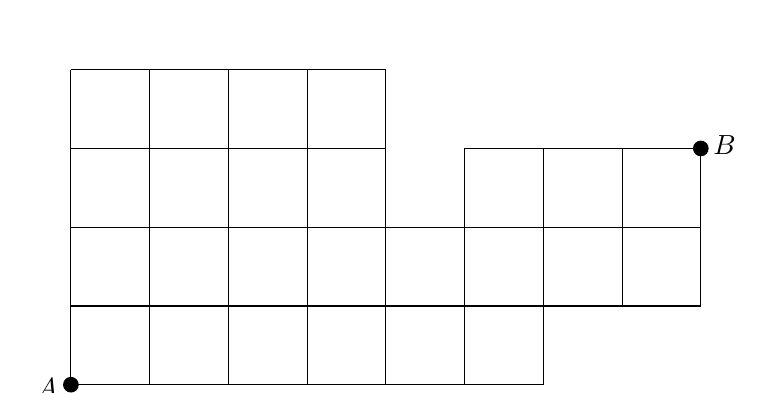
\begin{tikzpicture}
			      \draw (0,0) grid(4,4);
			      \draw (4,0) -- (6,0);
			      \draw (4,1) -- (8,1);
			      \draw (4,2) -- (8,2);
			      \draw (5,0) -- (5,3);
			      \draw (6,0) -- (6,3);
			      \draw (7,1) -- (7,3);
			      \draw (8,1) -- (8,3);
			      \draw (5,3) -- (8,3);
			      \node at (0,0) [circle,fill,inner sep=2pt]{};
			      \node at (-0.3,-0.04) {$A$};
			      \node at (8,3) [circle,fill,inner sep=2pt]{};
			      \node at (8.3,3.04) {$B$};
			      % \draw (6,0) grid(2,2);
		      \end{tikzpicture}
	      \end{center}
\end{enumerate}

\newpage
\subsection{ANALISIS KOMPLEKS}
\textbf{BAGIAN PERTAMA}
\begin{enumerate}
	\item Diketahui polinom $p(z)=a_0z^n+a_1z^{n-1}+\dots+a_n$ dengan bilangan $a_0,a_1,\dots,a_n$ menyatakan bilangan real. Jika $z_0=3-4i$ merupakan akar-akar dari polinom, maka salah satu akar lain yang pasti muncul adalah \dots
	\item Faktor polinom $z^4+1$ menjadi polinom dengan derajat lebih rendah, tetapi mempunyai koefisien real.
	\item Tentukan jari-jari konvergensi $$1-z^2+z^4-z^6+\dots$$
	\item Tentukan banyaknya akar persamaan $z^4-5z+1=0$ di $1\leq |z|\leq 2$.
	\item Diketahui fungsi analitik $$f(z)=\dfrac{2(z-2)}{z(z-4)}$$
	      dan tuliskan sebagai $\displaystyle f(z)=\sum_{n=0}^{\infty}a_n(z-1)^n$. Nilai $a_{100}$ adalah \dots
	\item Diketahui $z_1=-1+i$ dan $z_2=3+4i$. Bilangan kompleks $w$ berada pada penggalan garis yang mengghubungkan $z_1$ dan $z_2$. Jika $|w|=\sqrt{27}$, tentukan $w$.
	\item Hitung nilai dari $\displaystyle \int_{C}e^{(2/z)}\, dz$ bila $C$ adalah lingkaran satuan.
	\item Diketahui $C$ lingkaran berpusat di $O$. Tentukan nilai dari $\displaystyle \int_{C}\dfrac{1}{1-z}\, dz$ adalah $\dots$
\end{enumerate}
\newpage
\newpage \textbf{BAGIAN KEDUA}
\begin{enumerate}
	\item Diketahui $f$ fungsi \textit{entire} (analitik di seluruh daerah $\mathbb{C}$) dan diketahui pula ada bilangan bulat $k$, bilangan positif $A$ dan $B$ sehingga
	      $$|f(z)|\leq A+B|z|^k$$
	      Buktikan bahwa $f$ merupakan polinom dengan derajat paling tinggi adalah $k$.
	\item Tunjukkan bahwa:
	      $$P_n(z)=a_0z^n+a_1z^{n-1}+\dots+a_{n-1}z+a_n$$
	      sekurang-kurangnya mempunyai satu nilai nol.
	\item Buktikan $\ln(1+z)=z-\dfrac{z^2}{2}+\dfrac{z^3}{3}-\dfrac{z^4}{4}+\dots$ untuk $|z|<1$.
\end{enumerate}
\newpage \subsection{STRUKTUR ALJABAR}
\textbf{BAGIAN PERTAMA}
\begin{enumerate}
	\item Diketahui $G=\{1,-1\}$ grup dengan operasi kali dan $G^3=\{(a,b,c):a,b,c\in G\}$ grup dengan operasi untuk setiap $x_1=(a_1,b_1,c_1)$,$x_2=(a_2,b_2,c_2)\in G$ berlaku $$x_1*x_2=(a_1a_2,b_1b_2,c_1c_2).$$
	      Banyaknya subgrup dari $G^3$ dengan berorder 4 adalah \dots
	\item Penulisan permutasi $\phi=\left(\begin{array}{cccccccc}
			      1 & 2 & 3 & 4 & 5 & 6 & 7 & 8 \\8&2&6&3&7&4&5&1
		      \end{array}\right)$ sebagai dari permutasi siklik yang saling disjoin adalah \dots
	\item Perhatikan grup dihedral dengan order 8: $D_4=\{e,y,y^2,y^3,x,xy,xy^2,xy^3 \}$, $x^2=y^4=e$ dan $xy=y^{-1}x$. Grup $D_4$ ini mempunyai subgrup berorder 4 yang tidak siklik yaitu \dots
	\item Perhatikan ring kuosien $\mathbb{Z}_5[x]/I$ dengan $I$ adalah ideal yang dibangun oleh $h=x^3+3x+2$. Unsur $(x+2)/I$ di $\mathbb{Z}_5/I$ mempunyai balikan dengan balikannya adalah \dots
	\item Contoh ideal maksimal dari $\mathbb{Z}_{18}$ adalah \dots
	\item Perhatikan ring polinom $\mathbb{Z}_3[x]$ dan jika $f\in \mathbb{Z}_3[x]$ notasi $\langle f\rangle$ menyatakan ideal yang dibangun oleh $f$. Bila $c\in \mathbb{Z}_3$ sehingga $\mathbb{Z}_3[x]/\left\langle x^3+cx^2+1 \right\rangle $ membentuk \textit{field} adalah \dots
	\item Polinom $x^4+1$ di ring $\mathbb{Z}_5[x]$ dapat difaktorkan atas polinom tak tereduksi yaitu$\dots $
	\item Jika $F$ adalah \textit{field} dengan order 81 maka karakteristik $F$ adalah \dots

\end{enumerate}
\newpage
\newpage \textbf{BAGIAN KEDUA}
\begin{enumerate}
	\item Misalkan $G$ suatu himpunan tak kosong dan $*$ suatu operasi biner pada $G$ yang bersifat asosiatif dan untuk setiap $a,b\in G$ berlaku $a^2*b=b=b*a^2$. Buktikan bahwa $G$ adalah grup komutatif.
	      catatan : $a^2=a*a$
	\item Misalkan $R$ suatu ring dengan karakteristik $n$(hingga). Untuk setiap $a\in R$ notasi $$G(a)=\{ ka : k\in \mathbb{Z}\}$$ menyatakan subgrup siklik dari $R$ terhadap operasi tambah yang dibangun oleh $a$.
	      \begin{enumerate}
		      \item[(a)] Buktikan bahwa jika $R$ \textit{integral domain}  maka untuk setiap $a,b\in R$ dengan $a\neq 0$ dan $b\neq 0$ berlaku subgrup $G(a)$ dan $G(b)$ isomorfik.
		      \item[(b)] Apakah jika pada pernyataan a, di atas syarat $R$ \textit{integral domain} kita hilangkan. Pernyataan "untuk setiap $a,b\in R$ dengan $a\neq 0$ dan $b\neq 0$ berlaku subgrup $G(a)$ dan $G(b)$ isomorfik" masih berlaku? Jelaskan!

	      \end{enumerate}
	\item Dari $R$ ring dan himpunan tak kosong $J\subset R$ dibentuk himpunan $$N(J)=\{r\in R\mid rx=0.~~~~ \forall x\in J \}$$
	      \begin{enumerate}
		      \item[(a)] Tunjukkan $N(J)$ tidak kosong!
		      \item[(b)] Apakah $N(J)$ merupakan ideal? Jelaskan!
		      \item[(c)] jika  $J\subset J'\subset R$ apa yang dapat saudara simpulkan tentang hubungan $N(J)$ dan $N(J')$. Jelaskan!
	      \end{enumerate}
\end{enumerate}

\newpage
\subsection{ALJABAR LINIER}
\textbf{BAGIAN PERTAMA}
\begin{enumerate}
	\item Jika $A$ matriks berukuran $1999\times 2006$, maka nilai minimal $\text{rank}(A)+\text{nullitas}(A)$ adalah \dots
	\item Koordinat $x^2$ terhadap basis $\{x^2+x, x+1, x^2+1\}$ adalah $P_2$ adalah \dots
	\item Jika $T:\mathbb{C}\to\mathbb{C} $ adalah pemetaan linier $x\in \mathbb{C}$, maka $T(x)$ adalah $\dots$
	\item Sukubanyak karakteristik matriks $\left(\begin{array}{rrr}
			      1 & -2 & 3 \\4&5&-6\\-7&8&9
		      \end{array}\right)$ adalah \dots
	\item Jika $A=\left[\begin{array}{rr}
				      2 & 1 \\1&2
			      \end{array}\right]$, maka $A^{2006}=\dots$
	\item Misalkan himpunan vektor $\{u_1,u_2,u_3,u_4 \}$ di $\mathbb{C}^n$ bebas linier. Agar himpunan $\{u_1+\alpha u_2,u_2+\alpha u_3,u_3+\alpha u_4,u_4+\alpha u_1 \}$ bebas linier, skalar $\alpha$ adalah $\dots$
	\item Misalkan $X=\{(1,0,1),(1,1,0),(0,1,1) \}$ dan $P$ adalah proyeksi ortogonal pada $X$. Matriks representasi $P$ terhadap basis baku di ruang Euklid $\mathbb{R}^3$ adalah $\dots$
	\item Misalkan $a$ bilangan real sehingga matriks $\left[ \begin{array}{ccc}
				      1 & a & a \\a&1&a\\a&a&1
			      \end{array}\right]$ memiliki tiga nilai karakteristik real $\lambda_1\geq \lambda_2\geq \lambda_3>0$, maka $a$ harus terletak di dalam selang $\dots$

\end{enumerate}
\newpage
\newpage \textbf{BAGIAN KEDUA}
\begin{enumerate}
	\item Misalkan $x_1, x_2$ dan $x_3$ bilangan-bilangan real $x_1<x_2<x_3$. Pemetaan $T:P_2\to \mathbb{R}^3$ didefinisikan dengan aturan $$T(p(x))=\left[\begin{array}{c}
				      p(x_1) \\p(x_2)\\p(x_3)
			      \end{array}\right]$$
	      untuk setiap $p(x)\in P_2$.
	      \begin{enumerate}
		      \item[(a)] Tunjukkan bahwa  $T$ merupakan pemetaan linier!
		      \item[(b)] Periksa bahwa $T$ bijektif
	      \end{enumerate}
	\item Misalkan $A$ matriks berukuran $2\times2$ yang memenuhi $tr(A^2)=\left[ tr(A)\right]^2$
	      \begin{enumerate}
		      \item[(a)] Tentukan $\text{det}(A)$
		      \item[(b)] Jika $A$ tidak dapat didiagonalkan, tentukan $tr(A)$
	      \end{enumerate}
	\item Misalkan $\lambda$ adalah nilai karakteristik matriks $P$ yang memenuhi $P^t=P^2$. Tentukan semua $\lambda$ yang mungkin.
\end{enumerate}

\pagebreak

%============================================
%ONMIPA2007

\lhead{ONMIPA-PT(2007)}
\section{ONMIPA-PT TINGKAT WILAYAH 2007}

\subsection{ANALISIS REAL}

\textbf{BAGIAN PERTAMA}
\begin{enumerate}
	\item Diberikan $p$ adalah bilangan prima dan $A=\bigg \{-\dfrac{m}{n}-p\dfrac{n}{m}\bigg\}$. Tentukan $\text{sup}(A)$.
	\item Diberikan barisan $(y_n)$ dengan $y_1=1,~y_{n+1}=\dfrac{1}{4}\left(y_{n}^2+y_{n}^3\right)-1$. Tentukan $\displaystyle\lim_{n\to \infty}y_n$
	\item Diberikan barisan $(x_n)$ dengan $x_1=1$ dan $x_{n+1}=x_n^2+x_n$. untuk $n=1,2,3,\dots$. Didefinisikan barisan $y_n=\dfrac{1}{1+x_n}$, jumlah $\displaystyle S_n=\sum_{k=1}^{n}y_k$ dan hasil kali $\displaystyle P_n=\prod_{k=1}^{n}y_k$ untuk $n$ suku pertama dari $y_n$. Tentukan $S_n+P_n$ untuk $n=1,2,3,\dots$
	\item Diberikan $\theta_n=\arctan n$, maka $\displaystyle \lim_{n\to \infty}(\theta_{n+1}-\theta_n)=\dots$
	\item Tentukan $\displaystyle \lim_{n\to \infty}\sum_{k=1}^{n}\dfrac{1}{n}\sin\left(\dfrac{k\pi}{n}\right)$.
	\item Berikan contoh fungsi $f$ yang tidak memenuhi persyaratan: jika $f:[0,1]\to \mathbb{R}$ kontinu, maka terdapat konstanta $C$ dan $\varepsilon>0$ sehingga $$|f(x)-f(y)|\leq C|x-y|^\varepsilon.$$
	\item Diberikan fungsi $f:(0,1)\to \mathbb{R}$ terdiferensial di setiap $x\in(0,1)$ dan memenuhi persamaan $\displaystyle f(x)=f'(x)+\int_{0}^{1}f(x)\,dx$ untuk setiap $x\in(0,1)$. Jika terdapat $a,b\in(0,1)$ dengan $f(a)=f(b)=\dfrac{a+b}{2}$ maka $f\left(\dfrac{a+b}{2}\right)=\dots$
	\item Misalkan $f$ fungsi konveks pada $[0,2\pi]$ dengan $f^n(x)\leq M$. Tentukan nilai $a$ dan $b$ sehingga $$a\leq \int_{0}^{2\pi}f(x)\cos x\leq bM.$$
\end{enumerate}
\newpage \textbf{BAGIAN KEDUA}
\begin{enumerate}
	\item Diberikan $f,g:[a,b]\to \mathbb{R}$ fungsi kontinu dengan
	      $$\text{inf}\{f(x):x\in[a,b] \}=\text{inf}\{g(x):x\in[a,b] \}$$
	      Tunjukkan bahwa terdapat $c\in [a,b]$ sehingga $f(c)=g(c)$.

	\item Misalkan $f$ terbatas $a\leq x\leq b$ dan untuk setiap pasangan bilangan $x_1,x_2$ dengan $a\leq x_1\leq x_2\leq b$ berlaku $$f\left( \dfrac{1}{2}\left(x_1+x_2\right)\right)\leq \dfrac{1}{2}\left(f(x_1)+f(x_2)\right) $$
	      buktikan $f$ kontinu pada $a\leq x \leq b$.

	\item Diberikan $f:[a,b]\to \mathbb{R}$ kontinu dan terdiferensialkan secara kontinu, dan $m=\dfrac{f(b)-f(a)}{b-a}$. Tunjukkan bahwa $\displaystyle \int_{b}^{a}\left[f'(x)\right]^2\,dx\geq m^2(b-a)$ dan kesamaan berlaku jika dan hanya jika $f(x)=f(a)+m(x-a)$.
\end{enumerate}
\newpage
\newpage \subsection{KOMBINATORIKA}
\textbf{BAGIAN PERTAMA}
\begin{enumerate}
	\item Pada gerobak seorang penjual martabak manis tertulis, "menyediakan 1001 kombinasi taburan". Jika $t$ adalah banyaknya jenis taburan yang penjual tersebut sediakan, tentukan nilai terkecil yang mungkin untuk $t$.
	\item Dari ke-26 abjad, berapa banyak yang dapat dituliskan tanpa mengangkat pensil dan tanpa mengulangi goresan yang telah dibuat?
	      \begin{center}
		      A B C D E F G H I J K L M N O P Q R S T U V W X Y Z
	      \end{center}
	\item Dari $10^8$ graph pohon berlabel yang didefinsikan pada 10 titik, berapa banyak yang derajat setiap titiknya adalah 3 dan 1.
	\item $\displaystyle \sum_{j\leq k\leq i}(-1)^k\binom{i}{k}\binom{k}{j}=\dots$
	\item Banyaknya solusi bilangan bulat dari $x_1+x_2+x_3<16$, dengan $x_i\geq i$ untuk $i=1,2,3$ adalah \dots
	\item Tentukan formula rekursif untuk $c_n$ yang menyatakan banyakanya himpunan bagian dari $\{1,2,3,\dots,n\}$ yang tidak memuat dua bilangan yang berurutan.
	\item Sepotong kawat berukuran 1 meter dipotong secara acak menjadi 3 bagian. Berapa peluang ketiga bagian ini membentuk segitiga?
	\item Banyaknya pemetaan $f:\{ 1,2,\dots,2007\}\to \{2006,2007 \}$ sehingga $f(1)+f(2)+\dots+f(2007)$ ganjil adalah \dots

\end{enumerate}
\newpage
\newpage \textbf{BAGIAN KEDUA}
\begin{enumerate}
	\item Diberikan sebelas bilangan bulat berbeda. Buktikan bahwa dua di antara bilangan-bilangan tersebut memiliki selisih yang merupakan kelipatan 10.

	\item Diketahui bahwa mahasiswa A menyukai mata kuliah : Aljabar linier, Kombinatorika, dan Statistika; mahasiswa B menyukai mata kuliah: Aljabar linier, Analisis kompleks, Kombinatorika, dan Statistika; mahasiswa C menyukai mata kuliah: Aljabar linier, Analisis kompleks, Analisis Real, dan Struktur aljabar; mahasiswa D menyukai mata kuliah: Analisis kompleks, Kombinatorika ,dan Statisika; mahasiswa E menyukai mata kuliah: Aljabar linier, Analisis kompleks, dan Statistika; mahasiswa F menyukai mata kuliah: Aljabar linier, Analisis kompleks, dan Kombinatorika.

	      Periksa apakah mungkin untuk membuat korespondensi 1-1 antara keenam mahasiswa dengan keenam mata kuliah sehingga setiap mahasiswa berpasangan dengan sebuah mata kuliah yang disukainya.

	\item Kotak-kotak pada sebuah papan catur berukuran $n\times n$ diwarnai hitam dan putih sedemikian sehingga setiap kotak hitam bertetangga dengan sejumlah ganjil kotak hitam lainnya. Jika $p$ menyatakan banyaknya, buktikan bahwa $p$ ganjil jika dan hanya jika $n$ ganjil.
\end{enumerate}
\newpage
\newpage
\subsection{ANALISIS KOMPLEKS}
\textbf{BAGIAN PERTAMA}
\begin{enumerate}
	\item Diketahui bilangan kompleks $|a|<1$. Didefinisikan pemetaan $\varphi_a(z)=\dfrac{z-a}{1-\overline{a}z}$. Jika $|z|=1$, hitung $|\varphi_a(z)|$.

	\item Diketahui fungsi $f$ analitik di domain yang memuat cakram satuan $\{z:|z|\leq 1\}$ dan $a\in D^0$ dengan $f(a)=a$. Didefinisikan fungsi $g$ yang analitik di domain yang memuat cakram satuan dengan sifat $g(0)=0$ dan $|g(z)|=|f(z)|$ jika $|z|=1$.
	\item Diketahui $C$ adalah kurva di kuadran pertama dengan $|z|=2$ untuk setiap $z\in C$ dari $z=2$ sampai dengan $z=2i$. Jika $\left|\displaystyle\int_{C}\dfrac{dz}{z^2-1}\right|\leq ML$, tentukan nilai $M$ sekecil mungkin dan $L$ (nyatakan panjang kurva).

	\item Hasil pemetaan lingkaran $L:|z-1|=1$ oleh $w=\dfrac{i}{z+2i}$.

	\item Diketahui fungsi $f:\mathbb{C}\to\mathbb{C}$ analitik atau holomorfik. Kemudian untuk $a\in \mathbb{C}$ didefinisikan \\
	      $$f(z)=\begin{cases}
			      \dfrac{f(z)-f(a)}{z-a}~~~z\neq a \\A~~~~~~~~~~~~~~~~z=a
		      \end{cases}$$
	      tentukan nilai $A$ agar $f$ kontinu pada $\mathbb{C}$

	\item Diketahui $\gamma$ adalah lingkaran berpusat di 0 dan berjari-jari 2. Tentukan nilai dari $\displaystyle\int_{\gamma}\dfrac{dz}{z^2(z^2+1)}$.

	\item Tentukan nilai maksimum dan minimum dari modulus $z^2-z$ pada cakram $|z|\leq 1$.

	\item Diketahui $p(z)=z^3-3z^2+4z-5$ dan $q(z)=z^2(1+q(z))$ dengan $q(0)\neq -1$. Tentukan nilai residu dari $f(z)=\dfrac{p(z)}{q(z)}$ di $z=0$.
\end{enumerate}

\newpage \textbf{BAGIAN KEDUA}
\begin{enumerate}
	\item Diketahui $f(z)=u(x,y)+iv(x,y)$ entire (analitik pada seluruh bidang kompleks). Jika $u$ terbatas dan $v$ satu-satu, maka tunjukkan bahwa $\forall z_1\neq z_2\in \mathbb{C}$ berlaku $f(z_1)-f(z_2)\notin \mathbb{C}$.

	\item Misalkan $f$ fungsi entire dan $|f'(z)|\neq |z|$ untuk semua $z$. Perlihatkan bahwa $f(z)=az+bz^2$ dengan $|b|\neq 1$.

	\item Diketahui fungsi $f$ pada cakram satuan $D$ dan $|f(z)|<1$ pada $D$. Jika $a$ dan $b$ adalah titik tetap di $D$ $f(a)=a$ dan $f(b)=b$, gunakan lemma Scwartz untuk membuktikan $f(z)=z$.
\end{enumerate}

\newpage \subsection{STRUKTUR ALJABAR}
\textbf{BAGIAN PERTAMA}
\begin{enumerate}
	\item Diketahui $\mathbb{Z}_2\times\mathbb{Z}_2=\{(a,b)|a,b\in \mathbb{Z}_2\}$ grup terhadap operasi tambah. Banyaknya automorfisma di $\mathbb{Z}_2\times\mathbb{Z}_2$.

	\item Misalkan $field$ F berorder  $k$ dan $G=GL_n(F)$. Jika $Z(G)$ adalah senter dari $G$, yaitu  $Z(G)=\{g\in G|xg=gx,\forall x\in G \}$, maka banyaknya unsur di $Z(G)$ adalah \dots

	\item Unsur di $S_4$ yang berorder 12 adalah \dots

	\item Ideal di ring $M_2(\mathbb{Z}_2)$ yang dibangun oleh $x=\left(\begin{array}{ll}
				      1 & 0 \\0&0\\
			      \end{array}\right)$

	\item Jika $D$ adalah suatu integral domain dengan sifat untuk setiap $x\in D$ berlaku $x^2=x$, maka banyaknya unsur di $D$ adalah \dots

	\item Diketahui $\mathbb{Z}\left[i\right]=\{a+bi\mid a,b\in\mathbb{Z}\}$ daerah Euclid bulat Gauss dengan pemetaan $d:\mathbb{Z}-\{0\}\to \{1,2,3,\dots\}$ dan $d(a+bi)=a^2+b^2$ untuk semua $a+bi\in \mathbb{Z}-\{0\}$. Faktorisasi atas unsur prima dari $100\in \mathbb{Z}\left[i\right]$

	\item Ring $\mathbb{Z}_{15}$ bukan $unique~ factorisation~domain$. Sebagai contoh, ada dua faktorisasi atas prima yang berbeda dari polinom $x^2-3x+2$ di ring $\mathbb{Z}_{15}[x]$, yaitu $x^2-3x+2=(x-1)(x-2)$ dan $x^2-3x+2=\dots$

	\item Jika $field$ F hingga maka $F-\{0\}$ membentuk grup siklik terhadap operasi kali di $F$. Pembangun dari $F-\{0\}$ disebut elemen primitif dari $F$. Contoh elemen primitif dari $field$ $\mathbb{Z}_2[x]/(x^3+x+1)$adalah $\dots$

\end{enumerate}
\newpage \textbf{BAGIAN KEDUA}
\begin{enumerate}

	\item Misalkan $G$ suatu grup dan $K\subseteq G$ subgrup dari $G$ dengan indeks $K$ di $G$ yaitu $[G:K]=23$
	      \begin{enumerate}
		      \item Tentukan semua subgrup dari $G$ yang mengandung $K$.
		      \item Jika $G$ grup komutatif dan orde dari $K$ yaitu $|K|=5$ tunjukkan bahwa $G$ grup siklik.
	      \end{enumerate}

	\item Misalkan ring $R$ komutatif dan untuk setiap $a\in\mathbb{R}$ didefinisikan
	      $$ann(a)=\{x\in R\mid ax=0\}$$
	      \begin{enumerate}
		      \item Untuk setiap $a\in R$ buktikan bahwa $ann(a)$ ideal dari $R$
		      \item Jika $a,r,ar\neq 0$ dan $ann(a)$ ideal prima tunjukkan $ann(ar)$ juga ideal prima.
		            catatan : ideal $I\subset R$ disebut ideal prima jika untuk setiap $xy\in I$ berlaku $x\in I$ atau $y\in I$
	      \end{enumerate}

	\item Misalkan $\alpha \in \mathbb{R}$ dengan $\alpha\neq 0$ dan terdapat bilangan bulat positif $n$ sehingga $\alpha^{n}\in \mathbb{Q}$. Misalkan pula $g(x)$ polinomial monik berderajat terkecil di $\mathbb{Q}[x]$ sehingga $g(\alpha)=0$
	      \begin{enumerate}
		      \item Tunjukkan bahwa terdapat $h(x)\in\mathbb{Q}$ sehingga $x^n-\alpha^n=h(x)g(x)$.
		      \item Jika $deg(g(x))=m$ tunjukkan bahwa $g(0)=\pm a^m$.
	      \end{enumerate}

\end{enumerate}
\newpage
\subsection{ALJABAR LINIER}
\textbf{BAGIAN PERTAMA}

\begin{enumerate}
	\item Misalkan $B$ basis bagi ruang vektor $V$ atas $F$. Misalkan $T:V\to V$ linier dan memenuhi $\left[T(x)\right]=\left[\begin{array}{c}
				      x_1-x_2+x_3 \\x_2\\x_1-x_2\end{array}\right]$. Matriks penyajian (representasi) $T$ terhadap basis $B$ adalah $\left[T\right]_B=\dots$
	\item Misalkan $X=\left\lbrace(1,a,a),(a,1,a),(a,a,1)\right\rbrace\subseteq \mathbb{C}^3$. Syarat perlu dan cukup agar $X$ bergantung linier adalah $a\in \dots$

	\item Misalkan $V$ ruang vektor atas $F$ dan $f:V\to F$. Nilai terbesar $rank(f)$ yang mungkin adalah $\dots $

	\item Pemetaan linier $T:P_2\to P_3$ didefinisikan oleh $(T(f))(t)=t\dfrac{df(t)}{dt},\forall f\in P_2$. Suku banyak karakteristik $T$ adalah $p(x)=\dots$

	\item Diberikan matriks $A(x)=\begin{bmatrix}
			      x-1 & 3 \\4&x+3
		      \end{bmatrix}$. Nilai terkecil $\det(A(x))$ adalah \dots

	\item Matriks $\left[\begin{array}{lll}
				      a & 1 & b \\b&a&1\\1&b&a
			      \end{array}\right]\in M_3(\mathbb{R})$  adalah matriks ortogonal jika dan hanya jika $(a,b)=\dots$

	\item Misalkan $K$ dan $L$ dua subruang dari ruang vektor $V$ atas $F$. Jika $K\neq L$ dan $\text{dim}(K)=\text{dim}(L)=5$, maka dimensi subruang $K+L$ paling sedikit adalah \dots

	\item Banyak matriks bilangan bulat $A=\begin{bmatrix}
			      a & b \\c&d
		      \end{bmatrix}$ yang memenuhi $A^3=I$ dan $b+c=0$.
\end{enumerate}
\newpage
\newpage \textbf{BAGIAN KEDUA}
\begin{enumerate}
	\item Misalkan $A\in M_n(F)$ memenuhi $A^4=0$. Tunjukkan bahwa $I+A$ memiliki balikan dan berikan $(I+A)^{-1}$.

	\item Misalkan $A\in M_2(F)$ pemetaan $T_A: M_2(F)\to M_2(F)$ didefinisikan dengan $T_A(X)=AX-XA, \forall X\in M_2(F)$
	      \begin{enumerate}
		      \item Tunjukkan bahwa $T_A$ merupakan pemetaan linier.
		      \item Tunjukkan bahwa $null(T_A)\geq 2$.
	      \end{enumerate}
	\item Misalkan $V$ ruang vektor berdimensi hingga atas $F$ dan $\mathcal{L}(V,F)$ adalah himpunan semua pemetaan linier dari $V$ ke $F$. 	Jika $K$ subring dari $V$, didefinisikan
	      $$K^{0}=\{f\in \mathcal{L}(V,F)|f(x)=0,\forall x\in K\}$$
	      Buktikan bahwa $(K\cap L)^{0}=K^{0}+L^{0}$, untuk setiap subruang  $K,L$ dari $V$.
\end{enumerate}



%====================================
%ONMIPA 2008
\newpage
\section{ONMIPA-PT TINGKAT WILAYAH 2008}
\lhead{ONMIPA-PT(2008)}
\subsection{ANALISIS REAL}

\textbf{BAGIAN PERTAMA}
\begin{enumerate}
	\item Infimum dari himpunan $A=\left\lbrace 3^{2x}+3^{1/2x}: x>0\right\rbrace$ adalah $\dots$
	\item Misalkan fungsi $f:\mathbb{R}\to \mathbb{R}$ mempunyai limit $L$ di titik $x=0$. Jika $g:\mathbb{R}\to \mathbb{R}$ didefinisikan dengan $g(x)=f(ax^2+x),\forall x\in \mathbb{R}$ dan $a>0$, maka $\displaystyle\lim_{x\to 0}g(x)=\dots$

	\item Benar atau salah: Jika $\displaystyle \lim_{x\to a}g(x)=c$, maka $\displaystyle\lim_{x\to a}(g\circ f)(x)=c$. Jika salah, berikan contohnya.

	\item Diberikan barisan bilangan real $(a_n)$ yang didefinisikan dengan $(a_1)=\dfrac{1}{2}$, dan nilai $a_{n+1}=a_n+a_{n}^2$. Apakah $(a_n)$ konvergen? Jika ya, berapa nilai limitnya?

	\item Diketahui bahwa $p$ buah bilangan bulat non-negatif $a_1,a_2,a_3,\dots,a_p$ bersifat $a_i\leq a_{i-1}, i=1,2,3,\dots,p$. Nilai dari $\displaystyle\lim_{n\to \infty}\left(a_{1}^{n}+a_2^n+\dots+a_p^n\right)$ adalah $\dots$

	\item Misalkan $H$ adalah himpunan semua fungsi $f:\mathbb{R}\to \mathbb{R}$ dimana $f$ mempunyai turunan yang kontinu, $f(0)=0$, dan $f(1)=1$. Untuk sembarang $f\in H$, didefinisikan $l_f$ sebagai panjang grafik dari $f$ pada interval $[0,1]$. Nilai dari $\sup\{l_f\mid f\in H\}$ adalah \dots
\end{enumerate}

\newpage \textbf{BAGIAN KEDUA}
\begin{enumerate}
	\item Diberikan barisan $(x_n)$ yang konvergen ke $x$, dan selanjutnya didefinisikan barisan $(y_n)$ dengan
	      $$y_n=\dfrac{1}{n}\displaystyle\sum_{k=1}^{n}x_k.$$
	      Tunjukkan bahwa barisan $y_n$ juga konvergen ke $x$.

	\item Diketahui fungsi $f$, $f_n:\mathbb{R}\to \mathbb{R}, 	n=1,2,3,\dots$. Untuk sebarang barisan $\{x_n\}$ konvergen ke $x$ berakibat barisan $\{f_n(x_n)\}$ konvergen ke $f(x)$. Tunjukkan bahwa fungsi $f$ kontinu.

\end{enumerate}

\newpage \subsection{KOMBINATORIKA}

\textbf{BAGIAN PERTAMA}
\begin{enumerate}
	\item Banyaknya bilangan terdiri dari dua digit sehingga hasil kali kedua digitnya genap adalah \dots

	\item Banyaknya bilangan bulat positif yang menjadi faktor 510510 adalah \dots

	\item $\displaystyle \binom{n-1}{0}+\binom{n}{1}+\binom{n+1}{2}+\dots+\binom{n+r-1}{r}=\dots$

	\item Persamaan eksplisit untuk $g_n=\sqrt{g_{n-1}+g_{n-2}}$ dengan $g_1=1$ dan $g_2=3$ adalah \dots

	\item Pada bidang Cartesius kita ingin bergerak dari titik $(0,0)$ menuju titik $(9,7)$ dengan aturan: kita hanya boleh bergerak ke kanan atau ke atas. Cacah rute terpendek untuk bergerak dari titik $(0,0)$ ke $(9,7)$, bila rute dari titik $(3,3)$ ke $(3,4)$ tidak boleh digunakan adalah \dots

	\item Diketahui $A=\{0,1\}$. Cacah string dengan panjang $n$ di $A^n$ yang tidak memuat 01 adalah \dots

	\item Pada suatu kantong terdapat masing-masing 50 bola berwarna merah, kuning, dan hijau. Jika setiap menit Anda mengambil suatu bola dari kantong, pada menit ke $\dots$ dijamin anda mendapatkan 12 bola dengan warna yang sama.

	\item Banyaknya graph sederhana (tidak saling isomorfik) dengan cacat verteks $n,(n\geq 2)$ adalah \dots
\end{enumerate}

\newpage \textbf{BAGIAN KEDUA}
\begin{enumerate}
	\item Perlihatkan bahwa bila $n+1$ bilangan bulat dipilih dari himpunan $\{1,2,\dots,mn\}$ untuk suatu bilangan bulat $m\geq 2$, maka terdapat dua bilangan bulat yang selisihnya tidak lebih dari $m-1$.

	\item  Tunjukkan banyaknya cara menghubungkan $2n$ titik pada lingkaran berpasangan oleh $n$ tali busur yang tidak saling berpotongan adalah $\displaystyle \dfrac{1}{n+1}\binom{2n}{n}$.
\end{enumerate}
\newpage \subsection{ANALISIS KOMPLEKS}

\textbf{BAGIAN PERTAMA}
\begin{enumerate}
	\item Misalkan $1+z^2+z^4+z^6+\dots=a$ pada $|z|<1$, dan $a\in\mathbb{C}$. Hasil dari $$\dfrac{1}{z+1}\left(1+z+z^2+z^3+z^4+z^5+\dots\right)=\dots$$
	\item Misalkan $z$ terletak pada lingkaran $|z|=2$. Estimasi nilai
	      $$\left|\dfrac{z}{z^3-z^2-2z+2}\right|$$
	      adalah \dots

	\item Akar pangkat 3 dari $$\left(\dfrac{i-\sqrt{3}}{1+i\sqrt{3}}\right)^2$$adalah \dots

	\item Pada $\mathbb{C}:|z|\leq 3$. $\displaystyle \int_{\mathbb{C}}\dfrac{z}{(z^2-1)(z+2)^3}\,dz=\dots$

	\item Jika $C$ sepenggal garis yang menghubungkan titik $2\sqrt{2}$ dan titik $2i\sqrt{2}$, maka estimasi nilai $\left|\displaystyle \int_{C}\dfrac{z^2}{z^2+2}\,dz\right|=\dots$

	\item Prapeta dari garis $x+y-1=0$ oleh transformasi linier $T(z)=2iz+2-i$ adalah \dots

	\item $\displaystyle\int_{0}^{2\pi}\cos(x)\cos(2x)\cos(4x)\cos(8x)\dots\cos(2^{2008}x)\,dx=\dots$

	\item $\displaystyle \dfrac{1}{2\pi i}\int_{|z|=1}e^{\sin \frac{1}{z}}\,dz=\dots$

\end{enumerate}

\newpage \textbf{BAGIAN KEDUA}
\begin{enumerate}
	\item Misalkan $h(z)$ fungsi harmonik bernilai kompleks dan $zh(z)$ juga harmonik. Tunjukkan $h(z)$ analitik.

	\item Misalkan $f$ analitik $f'$ kontinu, dan $|f(z)-1|<1$ pada suatu daerah $D$. Tunjukkan bahwa $\displaystyle \int_{C}\dfrac{f'(z)}{f(z)-1}\,dz=0$. Untuk setiap kurva tertutup $C$ yang berada dalam $D$.


\end{enumerate}

\newpage \subsection{STRUKTUR ALJABAR}

\textbf{BAGIAN PERTAMA}
\begin{enumerate}
	\item Banyaknya polinom berderajat dua yang berbeda dalam $\mathbb{Z}_2[x]$ adalah $\dots$


	\item Misalkan $G=A(S)$. grup yang memuat semua permutasi dari $\{x_1,x_2,x_3\}$ dan $H=\{\sigma\in G\mid x_1\sigma=x_1\}$. Banyaknya koset kanan dari $H$ di $G$ adalah$\dots$

	\item Banyaknya pembagi nol dari $\mathbb{Z}_{2008}$ adalah $\dots$

	\item Suatu contoh pasangan grup yang tak komutatif $G$ dan $N\trianglelefteq G$ yang memenuhi $G/N$ grup komutatif adalah $(G,N)$ adalah $\dots$

	\item Contoh gelanggang $R$ dimana hukum pembatalan tidak berlaku yaitu terdapat $a,b,c\in R$, $a\neq 0$ sehingga $b\neq c$, tetapi $ab=ac$ adalah $\dots$

	\item Diberikan grup $G=\{(a,b)|a,b\in \mathbb{R},a\neq 0\}$ terhadap operasi biner $\ast$ yang didefinisikan $(a,b)\ast(c,d)=(ac,b+d)$ untuk setiap $(a,b),(c,d)\in G$. Banyaknya unsur yang berorder 2 di $G$ adalah $\dots$

	\item Bilangan $n\geq 2$ yang mengakibatkan $\mathbb{Z}_n$ grup terhadap operasi $\ast $ dengan $\overline{a}\ast\overline{b}=\overline{ab}+\overline{a}+\overline{b}$ untuk setiap $\overline{a},\overline{b}\in \mathbb{Z}_n$ adalah $\dots$

	\item Semua ideal dari $\mathbb{Z}_7\times\mathbb{Q}$ adalah $\dots$

\end{enumerate}

\newpage \textbf{BAGIAN KEDUA}
\begin{enumerate}
	\item Misalkan $G$ grup komutatif. Jika terdapat $a,b\in G, a\neq b$ sehingga $o(a)=o(b)=2$. Tunjukkan bahwa $o(G)$ merupakan kelipatan 4. Apakah hal ini tetap berlaku apabila $G$ bukan grup komutatif.

	\item Misalkan $a,b\in \mathbb{R},a\neq 0$. Misalkan $\psi_{ab}:\mathbb{R}\to \mathbb{R}$ didefinisikan $\psi_{ab}(x)=ax+b$. Misalkan $G=\{\psi_{ab}\mid a,b\in \mathbb{R},a\neq 0\}$ dan $N=\{\psi_{1b}\in G\}$. Tunjukkan  bahwa $G/N$ isomorfik dengan $\mathbb{R}-\{0\}$ (grup semua bilangan real tak nol terhadap operasi perkalian).


\end{enumerate}
\newpage \subsection{ALJABAR LINIER }
\textbf{BAGIAN PERTAMA}
\begin{enumerate}
	\item Pemetaan linier $T:\mathbb{R}^2\to\mathbb{R}^2$ didefinisikan melalui $T(\alpha,\beta)=(3\alpha-\beta,\alpha+3\beta),$ untuk setiap $(\alpha,\beta)\in\mathbb{R}^2$. Terhadap basis $\mathbb{B}=\{(1,1),(1,-1)\}$ bagi $\mathbb{R}^2$, matriks penyajian (representasi) $T$ adalah \dots

	\item Matriks tak singular $X\in M_n(F)$ dikatakan \textit{ortogonal} jika ke-$n$ baris $X$ membentuk sebuah himpunan ortonormal. Jika $A$ ortogonal, maka haruslah $\det(A)=\dots$

	\item Untuk matriks $X=[x_{ij}]\in M_n(F)$, didefinisikan $\text{tr}(X)=\displaystyle\sum_{i=1}^{n}x_{ii}$. Jika $A,B\in M_n(F)$, maka $\text{tr}(AB-BA)=\dots$

	\item Jika $E\in M_n(F)$ memenuhi $E^2=E$, balikan (invers) dari matriks $I+E$ adalah \dots

	\item Misalkan $U,V,W$ tiga ruang vektor atas lapangan $F$, dengan $\dim(U)=2008$ dan $\dim(V)=8002$. Misalkan $T:V\to W$ dan $S:W\to U$ pemetaan-pemetaan linier yang memenuhi $T$ satu-satu, $S$ pada dan Peta$(T)=\ker(S)$, maka $\dim(W)=\dots$

	\item Agar matriks $\left(\begin{array}{cc}
			      1 & c \\-1&3
		      \end{array}\right)$ mempunyai nilai karakteristik(eigen) real dan tidak dapat didiagonalkan, maka haruslah nilai $c=\dots$

	\item Nilai terbesar multiplisitas geometri dari sembarang nilai karakteristik real $\left(\begin{array}{ccc}
			      2 & x & 0 \\0&2&1\\0&0&2
		      \end{array}\right)$ adalah $\dots
	      $ \\

	\item Banyaknya matriks bilangan bulat $A=\left(\begin{array}{ll}
			      a & b \\0&c
		      \end{array}\right)$ yang memenuhi $A^2+A=2I$ dan $\det(A)=4$ adalah $\dots
	      $
\end{enumerate}

\newpage \textbf{BAGIAN KEDUA}
\begin{enumerate}
	\item Misalkan $V$ ruang vektor atas $F$ berdimensi $2m-1$ untuk suatu bilangan asli $m\geq 2$. Jika $M$ dan $N$ dua subruang dari $V$ dengan $\dim (M)=\dim(N)=m$, tunjukkan bahwa $M\cap N\neq\{0\}$.

	\item Misalkan $A=[a_{ij}]\in M_4(\mathbb{R})$ memenuhi $a_{ij}>0$ jika $j\equiv i+1\mod 4$ dan $a_{ij}=0$ jika $j\ne\ i+1\mod 4$.
	      \begin{enumerate}
		      \item Tunjukkan bahwa semua komponen $(I+A)^3$ positif.

		      \item Apakah ada matriks $A$ yang memenuhi semua syarat di atas sehingga $(I+A)^3$ singular?
	      \end{enumerate}
\end{enumerate}
\newpage




%============================================
%ONMIPA2009
\lhead{ONMIPA-PT(2009)}
\section{ONMIPA-PT TINGKAT WILAYAH 2009}
\subsection{ANALISIS REAL}

\textbf{BAGIAN PERTAMA}
\begin{enumerate}
	\item Nilai $k$ yang merupakan bilangan bulat terkecil yang memenuhi ketaksamaan $\left\lbrace 1+ \frac{1}{n}\right\rbrace^n < k$, untuk $n = 1,2,3,\dots$ adalah \dots

	\item Diberikan barisan bilangan real $\left<x_n\right>$, dengan $x_n \geq 0$ untuk setiap $n$. jika $\displaystyle\lim_{n \to \infty}\left(-1\right)^nx_n$ ada, maka $\left<x_n\right>$ konvergen ke \dots

	\item Suatu barisan bilangan real  $\left<a_n\right>$ didefinisikan dengan $a_0 > 0, a_1 > 0$, dan $a_{n+2} = 1 + \frac{a_{n+1}}{a_n}$. Apakah barisan $\left<a_n\right>$ konvergen$?$ Jika iya, berapakah nilai limitnya?

	\item Diketahui fungsi $f : \mathbb{R} \to \mathbb{R} $ dengan $f(x+y) = f(x)f(y),$ untuk setiap $x,y \in \mathbb{R}$. Jika $f$ kontinu di $x=0$ dan terdapat bilangan real $a$ dengan $g(a) = 0$, maka nilai $g(x)$ untuk setiap $x \in \mathbb{R}$ adalah \dots

	\item Contoh fungsi bernilai real $f$ dan $g$ diskontinu di $c$, tetapi $fg$ kontinu di $c$ adalah \dots

	\item Jika fungsi bernilai real $f$ kontinu pada $\left[a,b\right]$ dengan $\displaystyle\int_{a}^{b} f \,dx=  0$, syarat yang harus dipenuhi agar $f(x) = 0$ untuk semua $x \in \left[a,b\right]$ adalah \dots

	\item Misalkan interval $I \subseteq \mathbb{R} $ dan $c \in I$. Fungsi-fungsi $f$ dan $g$ terdefinisi pada $I$. Turunan kedelapan dari $f$ dan $g$, yaitu $f^{(8)} $ dan $g^{(8)} $, ada dan kontinu pada $I$. jika $f^{(k)}(c) = 0$ dan $g^{(k)}(c) = 0$, untuk $k = 0,1,2,3,\dots,7$, tetapi $g^{(8)}(c) \not= 0$, maka $\displaystyle\lim_{x \to c} \frac{f(x)}{g(x)}$ adalah $\dots$

	\item Diketahui fungsi $f,g : \mathbb{R} \to \mathbb{R}$ kontinu. Untuk sembarang himpunan $S \subseteq \mathbb{R},~ \overline{S}$ menyatakan \textit{closure} dari $S$, yaitu irisan dari semua himpunan tertutup yang memuat $S$. Jika $S = \left\lbrace x \in \mathbb{R} : f(x) \geq g(x) \right\rbrace$, maka $S = \dots$

\end{enumerate}

\newpage \textbf{BAGIAN KEDUA}
\begin{enumerate}
	\item Misalkan $f(x) = a_1 \sin x + a_2 \sin 2x +\dots+ a_n \sin nx$ dengan $a_1,a_2,\dots,a_n$ bilangan-bilangan real. jika $\left|f(x)\right| \leqslant \left|sin x\right|$ untuk semua $x$, buktikan bahwa
	      \begin{equation*}
		      \left|a_1+2a_2+\dots+na_n\right| \leqslant 1.
	      \end{equation*}


	\item Misalkan fungsi $f$ terdiferensial pada $\left[a,b\right], f'(x) \not= 0$ untuk semua $x \in (a,b)$ dan $f(a)=f(b)=0$. Buktikan bahwa terdapat $c \in \left[a,b\right] $ sehingga $$\left|f'(c)\right| \geq \frac{1}{K} \displaystyle\int_{a}^{b} f,$$ untuk bilangan positif $K$.
\end{enumerate}
\newpage \subsection{KOMBINATORIKA }
\textbf{BAGIAN PERTAMA}
\begin{enumerate}
	\item Banyaknya himpunan bagian dari $\left\lbrace a,b,c,d,e,f,g,h \right\rbrace$ yang memuat ketiga elemen $a,b, $ dan $f$ adalah $\dots$

	\item Pada setiap titik sudut segitiga $ABC$ diletakkan sebuah titik. Kemudian pada sisi $AB$ diletakkan 4 buah titik, pada sisi $BC$ diletakkan 5 buah titik dan pada sisi $AC$ diletakkan 7 titik, banyaknya segitiga yang dapat dibentuk dari titik-titik tersebut adalah \dots

	\item Untuk bilangan bulat $n \geq 1, \displaystyle \sum_{k=n}^{2n} \left( \begin{array}{c}
				      k \\n
			      \end{array} \right)2^{-k} =\dots$

	\item Banyaknya solusi bulat dari persamaan $a+b+c+d = 20$ dengan $a \geq 3,\, b \geq 1,\, c \geq 1, $ dan $d \geq 5$ adalah \dots

	\item Solusi dari relasi rekurensi $a_{n+1} = \dfrac{a_{n}}{1+na_{n}}$ dengan $a_0 = 1$ adalah \dots

	\item Bilangan bulat positif $n$ terbesar agar $2^n$ membagi koefisien dari $y^{10}$ pada ekspansi $(7y+5)^{100}$ adalah \dots

	\item Pada suatu pesta akan dibuat satu rangkaian hiasan buah yang terdiri dari buah salak, apel, dan jeruk. Paling sedikit berapa buah yang harus disediakan untuk menjamin pada rangkaian buah tersebut terdaapat 8 salak atau 6 apel, atau 9 jeruk?

	\item Banyak cara memilih 4 bilangan berbeda dari himpunan $$\left\lbrace 1,2,3,4,5,6,7,8,9,10  \right\rbrace$$ sehingga dari 4 bilangan terpilih tidak terdapat 2 bilangan berurutan adalah \dots


\end{enumerate}

\newpage \textbf{BAGIAN KEDUA}
\begin{enumerate}
	\item Dari 400 bilangan bulat $1,2,3,\dots,400$ dipilih 201 bilangan. Buktikan bahwa di antara 201 bilangan bulat terpilih terdapat 2 bilangan sehingga satu bilangan tersebut akan membagi bilangan yang lain.

	\item Diberikan barisan $a_1, a_2,\dots, a_{2n}$ yang terdiri dari $n$ buah 1 dan $n$ buah $-1$ dengan jumlah parsialnya memenuhi sifat
	      \begin{equation*}
		      a_1 + a_2 +\dots+ a_k, \geq 0 \,\,\,\,\, \space (k = 1,2,\dots,2n)
	      \end{equation*}
	      Perlihatkan bahwa banyaknya barisan yang demikian adalah $\dfrac{1}{n+1} \left( \begin{array}{c}
				      2n \\n
			      \end{array} \right) $.
\end{enumerate}

\newpage \subsection{ANALISIS KOMPLEKS}

\textbf{BAGIAN PERTAMA}
\begin{enumerate}
	\item Tuliskan bilangan kompleks $2009^i-i^{2009}$ dalam bentuk $a+bi$ dengan $a,b$ bilangan real.

	\item Tentukan fungsi linier entire (\textit{entire linier function}) yang membawa \textbf{segitiga} dengan titik sudut 0,1 dan $i$ menjadi \textbf{segitiga} sebangun dengan titik sudut $0,2,$ dan $i+1$.

	\item Misalkan $\mathbb{C}$ adalah himpunan semua bilagan kompleks $z$ yang memenuhi $|z|=\left|\dfrac{1}{z}\right|$, maka bilagan real terkecil $A$ yang memenuhi $|z-2i|\leq A$ untuk setiap $z\in \mathbb{C}$ adalah \dots
	\item Hitung nilai $\displaystyle \int_{C}\overline{z}\,dz$ dengan $C$ adalah lengkungan yang ada pada gambar berikut.
	      \begin{center}
		      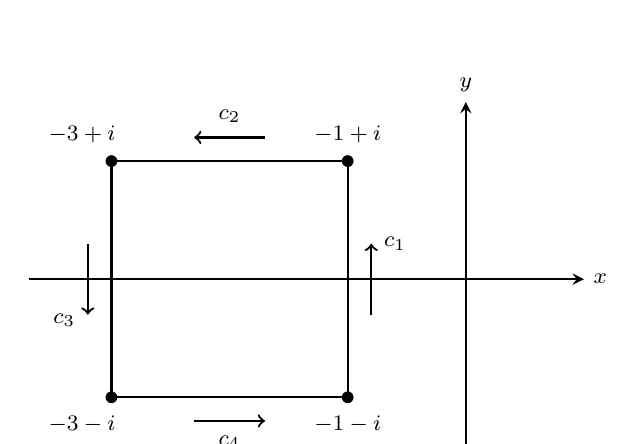
\begin{tikzpicture}[every node/.style={font=\footnotesize}]
			      \begin{axis}[x=1.5cm, y=1.5cm,ymin=-1.5,ymax=1.5,xmax=1,xmin=-3.7,xtick distance=5,  ytick distance=5,axis lines=middle,xlabel=$x$,ylabel=$y$,axis line style = thick,x label style={anchor=west},y label style={anchor=south}]
				      \node at (-1,1) [circle,fill,inner sep=1.5pt]{};
				      \node at (-3,1) [circle,fill,inner sep=1.5pt]{};
				      \node at (-3,-1) [circle,fill,inner sep=1.5pt]{};
				      \node at (-1,-1) [circle,fill,inner sep=1.5pt]{};
				      \draw[thick] (-3,1) -- (-3,-1) -- (-1,-1) -- (-1,1) -- (-3,1);
				      \draw[->,thick] (-0.8,-0.3) -- (-0.8,0.3);
				      \draw[->,thick] (-1.7,1.2) -- (-2.3,1.2);
				      \draw[->,thick] (-3.2,0.3) -- (-3.2,-0.3);
				      \draw[<-,thick] (-1.7,-1.2) -- (-2.3,-1.2);
				      \node at (-0.6,0.3){${c_1}$};
				      \node at (-1,1.23){$-1+i$};
				      \node at (-2,1.38){$c_2$};
				      \node at (-2,-1.38){$c_4$};
				      \node at (-3.25,1.23){$-3+i$};
				      \node at (-3.4,-0.35){$c_3$};
				      \node at (-3.25,-1.23){$-3-i$};
				      \node at (-1,-1.23){$-1-i$};
			      \end{axis}
		      \end{tikzpicture}
	      \end{center}
	\item Hitung nilai $\displaystyle \oint_{|z|=2}\dfrac{z+2}{z^3-3z^2}\,dz$ dengan arah lengkungan sesuai dengan arah gerak jarum jam.

	\item Hitung nilai $\displaystyle\int_{|z|=2}\dfrac{z+2}{z^2-z}\,dz=\dots$

	\item Hitunglah nilai $\displaystyle \oint_{C}z^2\exp\left(\dfrac{1}{z}\right)\,dz$ dengan $C$ adalah lengkungan $|z|=3$ dengan  arah jarum jam.

	\item Tentukan daerah konvergensi deret $\displaystyle\sum_{n=0}^{\infty}\left(z^n+\dfrac{1}{2^nz^n}\right)$.
\end{enumerate}

\newpage \textbf{BAGIAN KEDUA}
\begin{enumerate}
	\item Misalkan $f(z)$ fungsi analitik yang terdefinisi pada himpunan buka yang memebuat cakram satuan $\{z\mid |z|\leq 1\}$. Misalkan pula $u(x,y)=Re(f(z))$ yaitu bagian real dari nilai fungsi $f$ di titik $(x,y)$. Buktikan bahwa
	      $$\int_{C}\dfrac{\partial u}{\partial x}dy-\dfrac{\partial u}{\partial y}dx=0$$
	      dengan $C$ adalah lingkaran satuan.
	\item Diketahui deret $\displaystyle \sum_{n=0}^{\infty}c_nz^n$ mempunyai jari-jari konvergensi $R$, dan bilangan kompleks $z_0$. Tentukan jari-jari konvergensi deret
	      $$\sum_{n=0}^{\infty}\left(1+z_0^n\right)c_nz^n.$$
\end{enumerate}
\pagebreak
\newpage \subsection{STRUKTUR ALJABAR}

\textbf{BAGIAN PERTAMA}
\begin{enumerate}
	\item Diberikan $2$ bilangan bulat $a=2210$ dan $b=1131$. Pembagi persekutuan terbesar $d$ untuk $a$ dan $b$ dinyatakan sebagai $ax+by$ untuk suatu bilangan bulat $x$ dan $y$ adalah \dots

	\item Diberikan $n_1\mathbb{Z}, n_2\mathbb{Z},\dots,n_k\mathbb{Z}$ ideal-ideal dalam ring $\mathbb{Z}$. Kernel pemetaan $f:\mathbb{Z} \to \mathbb{Z}n_1 \times \mathbb{Z}n_2 \times \cdots \times \mathbb{Z}n_k$ yang didefinisikan dengan $r \mapsto (r (\mod\, n_1), r (\mod\, n_2) ,\cdots, r(\mod\,n_k))$ adalah \dots

	\item Diberikan $F$ lapangan, $f(x)$ adalah polinomial berderajat $n$ dalam $F[x]$ yang irredusibel dan $\alpha $ adalah suatu akar polinomial $f(x)$. Ideal yang dibangun oleh $f(x)$ dinotasikan sebagai $\left< f(x) \right>$. Jika $x$ dalam lapangan $F[x]/\left< f(x) \right>$ diganti dengan $\alpha$, maka $F[x]/\left< f(x) \right>$ dapat dinyatakan sebagai $F[\alpha]$, yaitu
	      \begin{center}
		      $F[\alpha] = \left\lbrace a_0+a_1\alpha+\dots+a_{n-1}\alpha^{n-1}\mid a_i \in F\right\rbrace $
	      \end{center}
	      Jika $F_2$ adalah lapangan dengan 2 elemen dan $f(x) = 1 + x + x^2$ maka elemen-elemen $F[x]/\left< f(x) \right>$ adalah \dots

	\item Banyaknya elemen idempoten dalam ring $\mathbb{Z}_{210}$ adalah \dots

	\item Diberikan $n$ suatu bilangan bulat positif. Didefinisikan $n\mathbb{R} {} = \left\lbrace nr \mid r \in \mathbb{R} \right\rbrace$ yang merupakan subgrup $\mathbb{R}$ terhadap operasi penjumlahan, maka $R/2009\mathbb{R}$ adalah \dots

	\item Misalkan $G = \left\lbrace e, \theta,a,b,c,\theta a,\theta b, \theta c \right\rbrace$ suatu grup dengan $a^2 = b^2 = c^2 = \theta$. $\theta ^2 = e$, $ab=\theta ba=c$, $bc = \theta cb = a, ca, \theta ac = b$. Senter dari $G$ adalah \dots

	\item Jika $F_1$ dan $F_2$ adalah lapangan, maka banyaknya ideal dari $F_1 \times F_2$ adalah \dots

	\item Misalkan $f$ adalah homomorfisma dari suatu grup siklis yang berorder 8 pada suatu grup siklik yang berorder 4. Ker $f$ adalah $\dots$
\end{enumerate}

\newpage \textbf{BAGIAN KEDUA}
\begin{enumerate}
	\item Diberikan $X$ suatu himpunan tak kosong, $K$ lapangan dan $K[X]$ ruang vektor semua fungsi pada $X$ yang bernilai-$K$. Adapun $S(x)$ menyatakan himpunan semua fungsi bijektif dari $X$ ke $X$. Jika $G$ sebarang grup aditif, maka aksi \textit{(action)} grup $G$ pada $X$ adalah suatu homomorfisma grup dari $G$ ke $S(x)$. Selanjutnya, didefinisikan pengaitan berikut
	      \begin{center}
		      $\psi : S(x) \to K[X], \sigma \mapsto \sigma\ast$.
	      \end{center}
	      dengan $\sigma\ast(f)(x):= f(\sigma ^{-1}x)$ untuk sebarang $f \in K[X]$
	      \begin{enumerate}
		      \item Buktikan $\psi$ merupakan homomorfisma grup.
		      \item Jika $S$ adalah aksi grup $G$ pada $X$, maka buktikan ada homomorfisma grup berikut:
		            \begin{center}
			            $S\ast : G \to K[X],  S\ast (g) = S(g)$.
		            \end{center}
	      \end{enumerate}


	\item Misalkan $G$ sebarang grup. Jika $a,b \in G$ maka komutator $a$ dan $b$ yang dinotasikan dengan $\left[a,b\right]$ adalah $aba^{-1}b^{-1}$. Kemudian dibentuk himpunan $A = \left\lbrace \left[a,b\right] \mid a,b \in G \right\rbrace$. Jika $G' = \left<A\right>$, maka buktikan $G'$ adalah subgrup normal dan $G/G'$ adalah grup komutatif.

\end{enumerate}
\newpage \subsection{ALJABAR LINIER}

\textbf{BAGIAN PERTAMA}
\begin{enumerate}
	\item Bentuk eselon tereduksi matriks $\left[\begin{array}{cccc}
				      1 & 2 & 3 & 4 \\5&6&7&8\\9&10&11&12
			      \end{array}\right]$ adalah \dots

	\item Misal $C(\mathbb R)$ menyatakan ruang fungsi kontinu dari $\mathbb R$ ke $\mathbb{R}$. Subruang $\{f \in C(\mathbb{R})\mid f"+f=0\}$ memiliki dimensi\dots

	\item Matriks persegi $A$ memenuhi $A^3 = 0$, maka matriks $A+2I$ tak singular dan $(A+2I)^{-1} = \dots$

	\item Misalkan $\left[\begin{array}{ccc}
				      2 & 1 & 3 \\1&0&1\\0&1&1
			      \end{array}\right]$. Didefinisikan pemetaan linier $T : \mathbb{R}^3 \to \mathbb{R}^3$ melalui $T(x) = Ax, \forall x \in \mathbb{R}^3$. Bilangan positif terkecil yang memenuhi $\mathbb{R}^3 = Peta(T^k)$ adalah \dots

	\item Misalkan $P_1$ ruang polinom real berderajat paling tinggi 1 dengan hasil kali dalam $\left< p(x),q(x) \right> = \displaystyle\int_{0}^{1} p(x)q(x)\,dx$. Proses ortonormalisasi Gram-Schmidt pada himpunan $\left\lbrace 1,x \right\rbrace$ di $P_1$ akan menghasilkan himpunan ortonormal \dots

	\item Misalkan $v = \left[\begin{array}{c}
				      2 \\1
			      \end{array}\right], A = \left[\begin{array}{cc}
				      v & v
			      \end{array}\right]$ dan $K = \left\lbrace x \in \mathbb{R}^2 \mid Ax = v \right\rbrace$, maka  $\min\left\lbrace ||x||_2 \mid x \in K \right\rbrace = \dots$

	\item Agar matriks $\left[\begin{array}{cc}
				      w & 1 \\-1&3
			      \end{array}\right]$ memiliki dua nilai eigen yang sama, haruslah $w = \dots$

	\item Contoh matriks real simetris $2\times2$ yang semua komponennya taknol dan semua nilai karakteristiknya negatif adalah $\dots$
\end{enumerate}

\newpage \textbf{BAGIAN KEDUA}
\begin{enumerate}
	\item Misalkan $e$ vektor di $\mathbb{R}^n$ yang semua komponennya 1. Tentukan det$(I-ey^T)$, untuk sembarang $y \in \mathbb{R}^n$. Tentukan semua $y$ yang membuat $I-ey^T$ singular.

	\item Misalkan $A$ matriks kompleks berukuran $m \times n$ dan $b \in \mathbb{C}^m$. Buktikan bahwa persamaan $Ax = b$ memiliki solusi jika dan hanya jika $b*y = 0$, untuk semua $y \in \mathbb{C}^m$ yang memenuhi $A*y = 0$.
\end{enumerate}
\newpage

\lhead{ONMIPA-PT(2010)}
\section{ONMIPA-PT TINGKAT WILAYAH 2010}
\subsection{ANALISIS REAL}
\textbf{BAGIAN PERTAMA}
\begin{enumerate}
	\item Misalkan himpunan $A = \left\lbrace \cos\dfrac{1}{n}+\left(-\dfrac{1}{n}\right) \bigg|~ n \in \mathbb{N} \right\rbrace$. Jika ada, $\sup A$ adalah \dots

	\item Berikan contoh fungsi bernilai real $f$ yang diskontinu $\forall x \neq 0$ pada domainnya, tetapi $f$ terdeferensialkan di $x=0$.

	\item Jika barisan bilangan real $(x_n)$ konvergen ke $x \in \mathbb{R} $ maka untuk $n \to \infty$
	      \begin{equation*}
		      \dfrac{x_1 + x_2 + x_3 +\dots+ x_n}{n}
	      \end{equation*}
	      konvergen ke \dots

	\item Diberikan fungsi-fungsi bernilai real $h$ dan $f$ dimana $f$ fungsi konveks. Syarat yang harus ditambahkan agar $f''(x)h(x) \geq 0, \forall x$ adalah \dots

	\item Nilai $z$ yang memenuhi sehingga deret
	      \begin{equation*}
		      1+(z-z^2)+(z-z^2)^2+(z-z^2)^3+\dots.
	      \end{equation*}
	      konvergen adalah \dots

	\item Misalkan turunan dari fungsi-fungsi $f$ dan $g$ kontinu dan $\displaystyle\lim_{n \to 0} f(x)=\displaystyle\lim_{n \to 0} g(x) = 0.$ Jika $g(x) \neq 0$ dan $g'(x) \neq 0$ untuk setiap $x$ dan $\displaystyle\lim_{n \to 0} \dfrac{f(x)}{g(x)} = L$, maka $\displaystyle\lim_{n \to 0} \dfrac{f'(x)}{g'(x)}$ adalah \dots

	\item Diketahui fungsi $f : \left[a,b\right] \to \mathbb{R}$ kontinu pada $\left[a,b\right]$ dan $c \in \left(a,b\right)$. Didefinisikan fungsi $g : \left[c,b\right] \to \mathbb{R}$, dengan $g(x) = \displaystyle\int_{c}^{x} f^2(t)\,dt$, untuk setiap $x \in \left[c,b\right]$. Diberikan sebarang $\epsilon >0$, nilai $\delta > 0$ yang dapat diambil agar setiap $x,y \in \left[c,b\right], |x-y| < \delta$, berlaku $|g(x)-g(y)|<\epsilon$ adalah \dots

	\item Nilai $\displaystyle\lim_{n \to \infty}  \displaystyle\int_{0}^{1} \left(\dfrac{x^{\frac{\pi}{2}}}{e^x} - e^x\right) dx$ adalah \dots

	\item Diketahui fungsi $f : \mathbb{R} \to \mathbb{R}$ kontinu dan $A \subseteq \mathbb{R} $. Hubungan $f(\overline{A})$ dan $\overline{f(A)}$ adalah . . . (Catatan: $\overline{A} = Cl (A)$)

	\item Misalkan fungsi $f$ terintegralkan dan kontinu seragam pada $\mathbb{R}$. Jika $(f_n)$ barisan fungsi terintegralkan yang didefinisikan dengan $f_n(x) = f\left(x + \dfrac{1}{n}\right)$, maka $\displaystyle \int_{0}^{1} f(x) \, dx = \dots$
\end{enumerate}

\newpage \textbf{BAGIAN KEDUA}
\begin{enumerate}
	\item Misalkan koefisien $a,b$ dan $c$ pada persamaan kuadrat $ax^2 + bx + c = 0$ merupakan bilangan rasional dan $a \neq 0$. Buktikan jika $\alpha = r + s \sqrt{2} $ merupakan akar persamaan tersebut, dengan $r$ dan $s$ rasional, maka $\beta = r-s\sqrt{2}$ juga merupakan akar.
\end{enumerate}

\newpage \subsection{KOMBINATORIKA}

\textbf{BAGIAN PERTAMA}
\begin{enumerate}
	\item Misalkan $A$ dan $B$ adalah himpunan bagian dari $\left\lbrace 1,2,\dots,6\right\rbrace$. Banyaknya pasangan berurut $(A,B)$ dengan $A \cap B = \emptyset$ adalah \dots

	\item Banyaknya bilangan asli kurang dari 1000 yang tidak habis dibagi 2, tidak habis dibagi 5, dan tidak habis dibagi 6 adalah \dots

	\item $\displaystyle\sum_{k = 0}^{100} k^2 \left( \begin{array}{c}
				      100 \\k
			      \end{array} \right) = \dots$

	\item Banyaknya solusi bulat dari persamaan $a+b+c+d = 18$ dengan $1 \leq a \leq 5 , -2 \leq b \leq 4, 0 \leq c \leq 5, 3 \leq d \leq 9, $ adalah \dots

	\item Solusi untuk formula rekursif $a_n = 4a_{n-2}, n \geq 2, a_0 =0, a_1 = 4$ adalah

	\item Banyaknya pemetaan pada (surjektif) yang dapat didefinisikan dari himpunan $A=\left\lbrace 1,2,3,4 \right\rbrace$ ke himpunan $B = \left\lbrace a,b,c \right\rbrace$ adalah \dots

	\item Suatu kotak berisi 100 buah permen CHA CHA yang terdiri dari 30 permen hijau, 20 permen orange, 10 kuning, 10 biru, dan 20 cokelat. Bila anda diminta mengambil permen dari kotak tersebut, minimal banyaknya permen yang harus diambil untuk menjamin bahwa anda pasti mendapatkan 13 permen dengan warna yang sama adalah \dots

	\item Pada ruang $xyz$ kita diizinkan untuk bergerak satu unit ke arah $x$ positif, ke arah $y$ positif, dan ke arah $z$ positif. Banyak cara yang mungkin ditempuh bila kita bergerak dari $(0,0,0)$ ke $(4,3,5)$ adalah

	\item Banyaknya pohon non-isomorfik yang memuat 7 titik adalah \dots

	\item Diberikan $k \geq 1$ adalah bilangan bulat dan $n$ adalah bilangan asli. Bila jumlahan dilakukan atas semua bulat tak negatif dari $n_1 + n_2 +\dots+ n_k = n$, maka nilai dari
	      \begin{equation*}
		      \displaystyle\sum \dfrac{n!}{n_1!n_2!\dots n_k!}
	      \end{equation*}
	      adalah  \dots

\end{enumerate}

\newpage \textbf{BAGIAN KEDUA}
\begin{enumerate}
	\item Buktikan bahwa dalam sebarang barisan yang terdiri dari $m$ bilangan bulat, terdapat satu atau beberapa suku-suku berturutan yang jumlahnya habis dibagi $m$.

	\item Pada papan tertulis sembilan angka 0, sepuluh angka 1, dan sebelas angka 2. Kita diperbolehkan untuk menghapus dua angka berbeda dan menuliskan sebuah angka yang lainnya. Sebagai contoh, kita menghapus angka 1 dan 2, dan menuliskan angka 0. Tunjukkan bahwa dengan melakukan serangkaian langkah ini, pada papan akan tersisa angka-angka yang sama. Angka manakah yang tersisa?
\end{enumerate}

\newpage \subsection{ANALISIS KOMPLEKS}

\textbf{BAGIAN PERTAMA}

\begin{enumerate}
	\item Tentukan nilai $5Re(z)+7lm(z)$ jika $z = (3-3i)^{2010}$.

	\item Tentukan Nilai
	      \begin{equation*}
		      \oint \dfrac{1}{z^3(z+4)} dz
	      \end{equation*}
	      dengan $C$ adalah lingkaran $|z+5|=3$.

	\item Dengan menggunakan $\displaystyle\oint_C \dfrac{dz}{z+1} $ dengan $C$ lingkaran $|z|=2$, hitung
	      \begin{equation*}
		      \oint \dfrac{(x+1)dx-ydx}{(x+1)^2 + y^2}
	      \end{equation*}

	\item Diketahui $f(z)= z^5 +2z^3-3iz^2+2z-1+i,$ hitung
	      \begin{equation*}
		      \oint_C \dfrac{f'(z)}{f(z)} dz
	      \end{equation*}
	      dengan $C$ adalah lingkaran yang melingkupi semua akar $f(z)$

	\item Misalkan $\left\lbrace a_n \right\rbrace$ barisan bilangan kompleks dengan $\sum |a_n|< \infty $ dan $\sum n|a_n|=\infty $. Tentukan jari-jari konvergensi deret $\sum a_n2^nz^n$.

\end{enumerate}

\newpage \textbf{BAGIAN KEDUA}
\begin{enumerate}
	\item Misalkan $f$ fungsi analitik di $z_0 \in \Omega $ dengan $f'(z_0) \neq 0$. Jika $C$ adalah lingkaran yang cukup kecil yang melingkari $z_0$, hitunglah
	      \begin{enumerate}
		      \item $\displaystyle\oint_C \dfrac{f(x)-f(z_0)}{(z-z_0)^2} dz$
		      \item $\displaystyle\oint_C \dfrac{1}{f(x)-f(z_0)} dz$
	      \end{enumerate}

	\item Tentukan peta himpunan
	      \begin{equation*}
		      A = \left\lbrace z \in \mathbb{C} : 1 < |z| < 3,0 < arg(z) < \dfrac{\pi}{6} \right\rbrace
	      \end{equation*}
	      oleh pemetaan $f(z)=-iz^3$.
\end{enumerate}



\newpage \subsection{STRUKTUR ALJABAR}

\textbf{BAGIAN PERTAMA}
\begin{enumerate}
	\item Kelipatan persekutuan terkecil dari 41327 dan 96577 adalah \dots

	\item Jika $R$ adalah suatu lapangan dengan identitas perkalian $1 \neq 0 $, maka ideal dari $R$ yang tak nol adalah \dots

	\item Diberikan tabel Cayley untuk operasi $*$ pada himpunan $H = \left\lbrace 0,1,2,3 \right\rbrace$ grup berikut ini
	      \begin{center}

		      \begin{tabular}{|c|c|}
			      \hline
			      * & 0 ~ 1 ~ 2 ~ 3       \\
			      \hline
			      0 & 0 ~ 1 ~ 2 ~ 3       \\
			      \hline
			      1 & 1 ~ $x$ ~ $a$ ~ $b$ \\
			      \hline
			      2 & 2 ~ $y$ ~ $z$ ~ $c$ \\
			      \hline
			      3 & 3 ~ $d$ ~ $e$ ~ $f$ \\
			      \hline
		      \end{tabular}

	      \end{center}
	      Agar $(H,*)$ merupakan grup yang tidak isomorfik dengan $(\mathbb{Z}_4, +)$ maka $(a,b,c) = \dots$

	\item Diketahui $F = \mathbb{Z}_2 [x] / \left< x^3 + x+1 \right>$. Invers perkalian dari elemen $\overline{x+1} \in F$ adalah \dots

	\item Banyaknya homomorfisma grup dari $\mathbb{Z}_6 $ ke $\mathbb{Z}_4$ adalah \dots
\end{enumerate}

\newpage \textbf{BAGIAN KEDUA}
\begin{enumerate}
	\item Misalkan $a,b$ bilangan-bilangan bulat. Buktikan bahwa terdapat bilangan-bilangan bulat $c$ dan $d$ yang memenuhi $(a+b\sqrt{2})(c+d\sqrt{2}) = 1$ jika dan hanya jika $a^2-2b^2 = 1$ atau $b^2-2a^2 = 1$.

	\item Himpunan $G$ adalah himpunan enam buah matriks real berukuran $3 \times 3$. Jika jumlah entri-entri pada setiap baris dan setiap kolom matriks tersebut adalah satu, carilah keenam matriks tersebut agar $G$ membentuk grup terhadap operasi perkalian matriks.
\end{enumerate}


\newpage \subsection{ALJABAR LINIER }

\textbf{BAGIAN PERTAMA}
\begin{enumerate}
	\item Jika $a,b,c$ adalah bilangan-bilangan real yang memenuhi
	      \begin{equation*}
		      a(1,0,2) + b(0,2,1) + c(1,2,3) = (2,-2,3)
	      \end{equation*}
	      maka $a+b+2c = \dots$

	\item Jika $K$ dan $L$ dua subruang dari $\mathbb{R}^{10}$ dan untuk $\dim K + \dim L = 12$, maka nilai terkecil yang mungkin untuk $dim(K \cap L)$ adalah \dots

	\item Diberikan basis $S = \left\lbrace (1,1,1),(1,1,0),(1,0,0) \right\rbrace$ bagi $\mathbb{R}^3$ dan vektor $\textbf{u} = (1,2,1) $ di $\mathbb{R}^3$. Koordinat $\textbf{u}$ terhadap basis $S$ adalah \dots

	\item Misalkan $A = \left[\begin{array}{ccc}
				      1 & 0 & 0 \\0&1&0\\-1&0&0
			      \end{array}\right]$.  Salah satu matriks real tak singular P yang membuat $P^{-1}AP$ matriks diagonal adalah \dots

	\item Matriks $A = [a_{ij}]$ matriks berukuran $2010 \times 2010$, dengan $ a_{ij} = \begin{cases} i,  \, i+j = 2011 \\0,  \, i+j \neq 2011
		      \end{cases}$, maka det $A = $\dots

	\item Misalkan $J : P_1 \to \mathbb{R}$ adalah tranformasi pengintegralan $J(p) = \displaystyle\int_{0}^{1} p(x)\,dx$, maka $Inti(J) = $\dots

	\item Diketahui matriks  $A = \left[\begin{array}{cc}
				      1 & 4 \\2&7
			      \end{array}\right]$ dan  $E = \left[\begin{array}{cc}
				      1 & -4 \\0&1
			      \end{array}\right]$, sedangkan $F$ dan $G$ adalah matriks-matriks dasar(elementer) sehingga $A^{-1} = EFG,$ maka $F-G = \dots$

	\item Untuk polinom-polinom $p = p(x)$ dan $q = q(x)$ di $P_2$, didefinisikan $$\left< p,q \right> = p(0)q(a) + p(\dfrac{1}{2})q(b)+p(1)q(c).$$
	      Untuk $a,b,$ dan $c$ tertentu $\left< \cdot,\cdot \right>$ merupakan sebuah hasil kali dalam pada $P_2$. Dengan norma yang berasal dari hasil kali dalam tersebut, $||4x^2-1||\dots$

	\item Misalkan $T_1 : \mathbb{R}^{3 \times 3} \to \mathbb{R}$ dan $T_2 : \mathbb{R}^{3 \times 3} \to \mathbb{R}^{3 \times 3}$ adalah transformasi linier dengan $T_2(A) = A^T.$ Jika $A = \left[ \begin{array}{ccc}
				      a & b & c \\d&e&f\\g&h&i
			      \end{array} \right]$ dan $(T_1 \circ T_2)(A) = T_1(A),$ maka $T_1(A) = \dots$

	\item Misalkan $A \in \mathbb{R}^{n \times n}$. Jika kolom kedua matriks $A$ merupakan kelipatan $k$ dari kolom keempat, maka salah satu pasangan karakteristik (pasangan eigen) untuk matriks $A$ adalah \dots


\end{enumerate}

\newpage \textbf{BAGIAN KEDUA}
\begin{enumerate}
	\item Misalkan $D$ menyatakan operator differensial pada $P_n$. Untuk $k = 2,3,4 ,\dots, n$ tuliskan $D^k = D \circ D \circ D \circ\dots \circ D$ yaitu komposisi $k$ buah $D$. Definisikan operator $T = I+D+D^2+\dots+D^n$ pada $P_n$
	      \begin{enumerate}
		      \item Tunjukkan bahwa $X = \left\lbrace 1 \right\rbrace \cup \left\lbrace x^k-kx^{k-1}\mid k=1,2,3,\dots,n \right\rbrace$ adalah basis bagi $P_n$
		      \item Periksa apakah $T$ pada. Berikan bukti untuk jawaban anda.
	      \end{enumerate}

	\item Misalkan $A \in \mathbb{R}^{n \times n}$ dan, untuk $i = 1,2,3,\dots,n, A_i$ adalah matriks berukuran $(n-1) \times (n-1)$ yang diperoleh dari matriks $A$ dengan menghilangkan baris dan kolom ke-$i$. Mislakan juga $p(t)$ dan $p_i(t)$ berturut-turut adalah polinom karakteristik matriks $A$ dan $A_i$, tentukanlah hubungan linier antara $\dfrac{dp(t)}{dt}$ dan $p_i(t)$, untuk $i=1,2,3,\dots,n$.
\end{enumerate}

\pagebreak

\lhead{ONMIPA-PT(2011)}
\section{ONMIPA-PT TINGKAT WILAYAH 2011}
\subsection{ANALISIS REAL}

\textbf{BAGIAN PERTAMA}

\begin{enumerate}
	\item Infimum dari himpunan $\left\lbrace n \in \mathbb{N} : (n!) \right\rbrace$ adalah \dots

	\item Misalkan $f,g : [0,1] \to \mathbb{R}^+$ adalah fungsi-fungsi injektif yang diferensiabel. Definisikanlah sebuah kombinasi fungsi dari $f$ dan $g$ sehingga dipenuhi sifat : jika $f(0) = g(1) = 0$, maka terdapat $c \in (0,1)$ sedemikian hingga $\displaystyle \left| \dfrac{(u(c))}{(v(c))}\right| = 2011 $, untuk $u(x) = \ln f(x)$ dan $v(x) = \ln g(x), \forall (0,1)$.

	\item Jika fungsi non-negatif $f$ terintegralkan Riemann pada $[a,b]$ dan $0 \leq m \leq f(x) \leq M, x \in [a,b]$, tentukan nilai $c$ dan $d$ sehingga $c \leq (\int_{a}^{b} f^2) \leq d$.

	\item Barisan $(S_n)$ dengan $S_n = \left(\dfrac{1}{n}\right)^n + \left(\dfrac{2}{n}\right)^n +\dots + \left(\dfrac{n}{n}\right)^n$ konvergen ke \dots

	\item Beri contoh suatu barisan dari fungsi-fungsi kontinu $(f_n)$ yang terdefinisi pada $[0,1]$, sedemikian sehingga $0 \leq f_n(x) \leq 1$, dan $\lim_{n \to \infty} \int_{0}^{1} f_n(x)\,dx = 0$, tetapi barisan tersebut tidak konvergen pada $[0,1]$.

	\item Jika $\left\lbrace a_n \right\rbrace $ barisan dengan $a_{n+1} = a_n + \dfrac{(2-a)}{(2a+1)}$ untuk setiap $n$, maka $\lim_{n \to \infty} a_n = \dots$

	\item Diketahui fungsi $f : [0,1] \to \mathbb{R} $ kontinu. Jika $f(x)$ rasional, untuk setiap $x \in [0,1]$, dan $f(0) = 0$, maka nilai $f\qty(\dfrac{\sqrt{2}}{4}) = \dots$
	\item Contoh fungsi $f$ dan $g$ yang kontinu seragam pada interval $I$, tetapi hasil kali keduanya tidak kontinu seragam pada $I$ adalah \dots

	\item Diketahui $I \subseteq \mathbb{R}$ interval dari $f : I \to \mathbb{R}$ fungsi. Jika $c$ titik interior ($interior~point$) $I$ dan untuk setiap $x,y \in I$, dengan $x < y,$ berlaku $f(x) \geq f(y)$, maka $\lim_{x \to c} f(x) = \dots$

	\item Jika $f''(x) + p(x)f(x)=0$ dan $g''(x)+p(x)g(x)=0$ untuk setiap $x \in (a,b)$, maka $W = f'g-fg' =\dots$ pada $(a,b)$
\end{enumerate}

\newpage \textbf{BAGIAN KEDUA}

\begin{enumerate}
	\item Diketahui himpunan $E \subset \mathbb{R}$ tertutup dan fungsi $f : E \to \mathbb{R}$ kontinu. Jika $\left\lbrace x_n \right\rbrace$ merupakan barisan Cauchy di dalam $E$, tunjukkan terdapat $c \in E$, dengan $\left\lbrace f(x_n) \right\rbrace$ konvergen ke $f(c)$.

	\item Jika fungsi $f:(0,1) \to \mathbb{R}$ kontinu dan terbatas, tunjukkan bahwa fungsi \(g : (0,1) \to \mathbb{R}\) dengan $g(x) = x(1-x)f(x),$ kontinu seragam.

	\item Jika fungsi $f : \mathbb{R} \to \mathbb{R}$ terdiferensial dan terdapat $c \in \mathbb{R}$ dengan $\lim_{x \to \infty} f'(x) = c,$ Tunjukkan bahwa
	      \begin{equation*}
		      \displaystyle\lim_{x \to \infty} \dfrac{f(x)}{x} =c.
	      \end{equation*}

\end{enumerate}
\newpage \subsection{KOMBINATORIKA}

\textbf{BAGIAN PERTAMA}
\begin{enumerate}
	\item Pada sebuah permutasi acak dari 26 huruf $\left\lbrace a,b,c,d,\dots,z \right\rbrace$, peluang bahwa huruf $b$ muncul tepat setelah huruf a adalah \dots

	\item Misalkan $A$ adalah himpunan dengan $n$ elemen dan $B$ adalah himpunan dengan $m$ elemen dengan $m \leq n$. Banyaknya pemetaan satu-satu (injektif) dari $B$ ke $A$ adalah \dots

	\item Solusi formula rekursif $v_n = v_{n-1} + n!n$ dengan $v_0 = 0$ untuk semua $n \in \mathbb{Z}^+$ adalah \dots

	\item Misalkan $n$ adalah bilangan delapan digit yang disusun dari enam digit berbeda dengan digit pertama adalah digit 5. Bila $n$ memuat tiga digit yang sama tetapi bukan digit 5, maka banyaknya cara menyusun $n$ terdapat adalah \dots

	\item Koefisien dari $x^{104}$ dalam ekspansi $\left( x - \dfrac{3}{5x} \right)^{210}$ adalah \dots

	\item Misalkan $\pi$ adalah sebuah permutasi atas himpunan $\left\lbrace 1,2,3,\dots,8 \right\rbrace$. Banyaknya permutasi $\pi$ sehingga bilangan genap tidak dipetakan ke dirinya sendiri adalah \dots

	\item Untuk setiap $m,n,k \in \mathbb{N}$, nilai dari
	      \begin{center}
		      $
			      \left( \begin{array}{c}
				      m \\0
			      \end{array} \right)
			      \left( \begin{array}{c}
				      n \\k
			      \end{array} \right) +
			      \left( \begin{array}{c}
				      m \\1
			      \end{array} \right)
			      \left( \begin{array}{c}
				      n \\k-1
			      \end{array} \right)+\dots +
			      \left( \begin{array}{c}
				      m \\k
			      \end{array} \right)
			      \left( \begin{array}{c}
				      n \\0
			      \end{array} \right) =\dots.
		      $
	      \end{center}

	\item Misalkan $\alpha $ adalah sebuah barisan $a_1, a_2,\dots , a_{20}$ dengan nilai $a_i$ adalah $1$ atau $0$ untuk semua $i = 1,2,3,\dots,20$. Misalkan $X = \left\lbrace \alpha : a_1 +a_2+\dots+a_{20} = 10 \right\rbrace$. Banyaknya barisan $\alpha$ sehingga $a_1 + a_2 +\dots+ a_{10} \in \left\lbrace 0,1,2 \right\rbrace$ adalah \dots

	\item Misalkan $1 \leq n \leq 2011 $ dengan $n $ bilangan asli yang memuat digit 0. Banyaknya $n$ yang demikian adalah \dots

	\item Jumlah semua bilangan desimal 0, $xyz$ dimana $x,y,$ dan $z$ merupakan tiga digit yang berbeda adalah \dots
\end{enumerate}

\newpage \textbf{BAGIAN KEDUA}
\begin{enumerate}
	\item Tentukan banyaknya bilangan bulat dari 1 sampai 99999 sehingga jumlah digit-giti pada bilangan tersebut adalah 22.

	\item Pada suatu acara seminar matematika dihadiri oleh $n$ orang peserta seminar. Tunjukkan bahwa antara para peserta seminar tersebut, senantiasa terdapat dua orang peserta seminar yang mempunyai jumlah kenalan yang sama.

	\item Sebuah graf dikatakan $k-$reguler bila setiap titik mempunyai derajat $k$. Sebuah \textit{perfect matching} dari sebuah graf dengan $n$ titik adalah himpunan $n/2$ sisi yang saling asing. Perlihatkan bahwa bila $G$ adalah sebuah graf bipartit $k-$reguler, maka $G$ mempunyai \textit{perfect matching}.
\end{enumerate}

\newpage \subsection{ANALISIS KOMPLEKS}

\textbf{BAGIAN PERTAMA}
\begin{enumerate}
	\item Tentukan jari-jari konvergensi deret
	      \begin{equation*}
		      \sum_{n = 1}^{\infty} \left[ \dfrac{z(z+n)}{n} \right]^n.
	      \end{equation*}

	\item Tentukan luas daerah peta dari hasil pemetaan daerah
	      \begin{equation*}
		      \left\lbrace z = x + iy \in \mathbb{C} | -1 < x \leq 2, -1 \leq y \leq 3 \right\rbrace
	      \end{equation*}
	      oleh tranformasi linier $T(z)=\left(1+i\sqrt{3}\right)z + 2 - i$.

	\item Berapakah nilai integral berikut
	      \begin{equation*}
		      \displaystyle\int_{|z-a| = a}^{} \dfrac{zdz}{z^4-1}~,~ a\in \mathbb{R}~,~ a>1.
	      \end{equation*}

	\item Misalkan $f(z)$ fungsi analitik yang memenuhi $|f(z)| \leq 1 + |z|^{3/2}$. Tuliskan semua fungsi analitik yang mungkin.

	\item Misalkan $p(z) = \sum_{n=0}^{\infty} a_nz^n$ dan $q(z) = \sum_{n=0}^{\infty} b_nz^n$. Selanjutnya didefinisikan $f(z)=p(z)q(z)$. Hitung $f^{(n)}(0)$, yaitu nilai turunan ke $n$ untuk fungsi $f$ di titik nol. Nyatakan nilai tersebut dalam $\left\lbrace a_k \right\rbrace $ dan $\left\lbrace b_k \right\rbrace$.

\end{enumerate}

\newpage \textbf{BAGIAN KEDUA}
\begin{enumerate}
	\item Buktikan bahwa jika $z_1 + z_2 +z_3 = 0$ dan $|z_1|=|z_2|=|z_3|=1$ maka $z_1. z_2, z_3$ adalah titik-titik ujung dari sebuah segitiga sama sisi yang berada di dalam lingkaran satuan.

	\item Misalkan $f(z) = \sum_{n = 0}^{\infty} c_nz^n$ fungsi analitik dengan jari-jari konvergensi $R$ dan di bidang kompleks hanya mempunyai satu pole order dua titik di $z_0$
	      \begin{enumerate}
		      \item Definisikan suatu fungsi analitik $F(z)$ yang analitik di seluruh bidang $\mathbb{C}$ yang diperoleh dari hasil perkalian $f(z)$ dengan suatu fungsi yang sederhana

		      \item Misalkan $F(z)=\sum_{n=0}^{\infty} d_nz^n$, berdasarkan hubungan yang diperoleh di soal (a), hitung nilai $c_n$ dinyatakan dalam suku-suku dari barisan $\left\lbrace d_k \right\rbrace_{k=1}^{\infty}$

		      \item Hitung $\dfrac{c_n}{c_{n+1}}$ dan $\displaystyle\lim_{n\to\infty} \dfrac{c_n}{c_{n+1}}$
	      \end{enumerate}
\end{enumerate}


\newpage \subsection{STRUKTUR ALJABAR}

\textbf{BAGIAN PERTAMA}
\begin{enumerate}
	\item Jika $G$ sebuah grup dengan subgrup $H$ sedemikian sehingga $|G| < 45, |H|>10 $ dan $|G:H|>3,$ maka $|G|=\dots$

	\item Diberikan $\mathbb{Z}_2$ sistem bilangan bulat modulo 2 dan himpunan $G$ yang unsur-unsurnya matriks $2 \times 2$ dengan komponen di $\mathbb{Z}_2$ dan determinan tak nol. Banyaknya subgrup berorde 2 adalah \dots

	\item Misalkan $S_5$ adalah grup simetri berorde 5. Orde dari $(12)(345)$ di $S_5$ adalah \dots

	\item Misalkan $R$ suatu ring dan $F$ suatu lapangan. Jika $\theta : F \to R$ homomorfisma ring yang tidak nol maka $Inti(\theta)=\dots$

	\item Perhatikan ring polinom $\mathbb{Z}_3[x].$ Bilangan $c \in \mathbb{Z}_3$ sehingga $x^3 + cx + 1$ tidak tereduksi di $\mathbb{R}_3[x]$ adalah \dots
\end{enumerate}

\newpage \textbf{BAGIAN KEDUA}
\begin{enumerate}
	\item Misalkan $G$ suatu grup dan $N$ subgrup dari $G$. Buktikan perkalian $(Na)\cdot (Nb) = N(ab)$ pada himpunan koset kanan dari $H$ terdefinisi dengan baik (\textit{well defined}) jika dan hanya jika $N$ subgrup normal dari $G$.

	\item Misalkan $R$ suatu gelanggang komutatif. Misalkan $r \in R$, didefinisikan $\rho_r : R \to R$, dimana $\rho_r(a)=ar$ untuk setiap $a \in R$. Buktikan $R$ daerah integral jika dan hanya jika $Inti(\rho_r)=\left\lbrace 0 \right\rbrace$ untuk setiap $r \in R - \left\lbrace 0 \right\rbrace$.

\end{enumerate}


\newpage \subsection{ALJABAR LINIER}

\textbf{BAGIAN PERTAMA}
\begin{enumerate}
	\item Diketahui bahwa $V$ adalah subruang dari $P_3$ yang dibangun oleh $$\left\lbrace x^3 + x^2, x^3+x, x+1, x^2+1 \right\rbrace,$$ maka dimensi $V$ adalah \dots
	\item Misalkan $A = [a_{ij}]$ matriks berukuran $2011 \times 2011.$ Jika $a_{ij} = i+j$ untuk setiap $i,j$, maka $rank(A) = \dots$

	\item Bidang $B$ di $\mathbb{R}^3 $ melalui titik-titik $(1,0,0),(0,1,0),$ dan $(0,0,-1)$. Vektor satuan yang tegak lurus terhadap bidang $B$ adalah \dots

	\item Diberikan vektor-vektor $x_1 = (1,1,0), x_2 = (0,1,1) $ di $\mathbb{R}^3$. Proses ortonormalisasi Gram-Schmidth pada $x_1, x_2$ menghasilkan vektor-vektor $v_1, v_2$, maka $v_2 = \dots$

	\item Misalkan $A$ dan $B$ matriks-matriks real berukuran berturut-turut $4 \times 2$ dan $2 \times 4$. Jika
	      \begin{center}
		      $AB = \left[ \begin{array}{cccc}
					      1  & 0  & -1 & 0  \\
					      0  & 1  & 0  & -1 \\
					      -1 & 0  & 1  & 0  \\
					      0  & -1 & 0  & 1  \\
				      \end{array} \right]$
	      \end{center}
	      maka $BA =\dots$

	\item Misalkan $T : P_2 \to \mathbb{R}$ adalah transformasi linier yang didefinisikan sebagai
	      \begin{equation*}
		      T(P(x)) = \displaystyle\int_{0}^{1} p(x) \,dx, ~~~ \forall p(x) \in P_2,
	      \end{equation*}
	      maka dimensi $Inti(T)$ adalah \dots

	\item Mislkan $\textbf{v} = (1,-2,4), \textbf{w}=(-3,6,k) \in \mathbb{R}^3$. Jika tidak ada $\textbf{u} \in \mathbb{R}^3$ sehingga $\textbf{w}$ adalah hasil proyeksi $\textbf{u}$ pada $\textbf{v}$, maka himpunan semua nilai $k$ yang mungkin adalah \dots

	\item Misalkan $\mathbb{R}^3 \times \mathbb{R}^3 \to \mathbb{R}$ didefinisikan sebagai $f(x,y) = x_1y_1 - x_2y_2 + 3x_3y_3$, untuk setiap $x = (x_1,x_2,x_3), y = (y_1,y_2,y_3) \in \mathbb{R}^3$, maka $f$ \underline{bukan} hasil kali dalam di $\mathbb{R}^3$ karena tidak memenuhi sifat \dots

	\item Misalkan matriks $A \in \mathbb{R}^{n \times n}$. Jika $A$ mempunyai $k$ kolom yang sama, maka dimensi ruang eigen $A$ untuk nilai eigen $\lambda = 0$ paling sedikit adalah \dots

	\item Misalkan $T$ operator linier pada $\mathbb{R}^{2 \times 2}$ yang didefinisikan sebagai
	      \begin{equation*}
		      T \left( \left[ \begin{array}{cc}
				      a & b \\c&d
			      \end{array} \right] \right) = \left[ \begin{array}{cc}
				      c & a \\d&b
			      \end{array} \right], \forall \left[ \begin{array}{cc}
				      a & b \\c&d
			      \end{array} \right] \in \mathbb{R}^{2 \times 2}
	      \end{equation*}
	      Jika $A$ adalah vektor eigen $T$ untuk nilai eigen $-1$, maka $\det(A) = \dots$
\end{enumerate}

\newpage \textbf{BAGIAN KEDUA}
\begin{enumerate}
	\item Misalkan $A = [a_{ij}]$ matriks berukuran $2011 \times 2011$ dengan
	      \begin{equation*}
		      a_{ij} = \begin{cases}
			      (-1)^{|i-j|}, ~~ for	~~ i \neq j \\
			      2, 	\hspace{1.5cm}			 for 	~~ i = j.
		      \end{cases}
	      \end{equation*}
	      Tentukan $\det(A).$

	\item Misalkan $G$ operator linier pada $\mathbb{R}^{2 \times 2}$ yang memetakan $A \in \mathbb{R}^{2 \times 2}$ ke $G(A) = A^T$, yaitu transpose dari $A$. Periksa apakah $G$ dapat didiagonalkan. Jika ya, berikan diagonalisasi dari $G$.

	\item Misalkan $V$ adalah subruang dari $\mathbb{R}^{50}$ yang dibangun oleh vektor-vektor $$\textbf{v}_1, \textbf{v}_2,\dots,\textbf{v}_{50}$$ adalah himpunan bilangan $\left\lbrace 1,2,\dots, 2500 \right\rbrace$, tentukan nilai terkecil dan nilai terbesar yang mungkin untuk $\dim(V)$.
\end{enumerate}

\newpage

\lhead{ONMIPA-PT(2012)}
\section{ONMIPA-PT TINGKAT WILAYAH 2012}
\subsection{ANALISIS REAL}
\textbf{BAGIAN PERTAMA}
\begin{enumerate}
	\item Diberikan $D \in \mathbb{R}$ dan fungsi $f,g : D \to \mathbb{R}$, dengan $f(x) \leq g(x)$, untuk setiap $x \in D.$ Beri contoh $D$, fungsi $f$ dan $g$ sehingga tidak benar bahwa $\sup \left\lbrace f(x) : x \in D \right\rbrace \leq \inf \left\lbrace g(x) : x \in D \right\rbrace$ .

	\item Diketahui $\left\lbrace a_n \right\rbrace$ barisan bilangan real dengan $a_1 > 0$ dan $a_{n+1} = \dfrac{1}{2+a_n}$ untuk setiap $n \geq 2$, \(\displaystyle\lim_{n \to \infty} a_n = \dots\)

	\item Diketahui fungsi $f : (a,b) \to \mathbb{R}$ terdiferensial hingga tingkat berapapun di $c \in (a,b).$ Nilai
	      \begin{equation*}
		      \displaystyle \lim_{h \to 0} \dfrac{f(c+h) - 2f(c)+f(c-h)}{h^2}
	      \end{equation*}

	\item Contoh fungsi $f$ yang memenuhi $|f(x)-f(y)| \leq (x-y)^2$, untuk setiap $x,y \in \mathbb{R}$ adalah \dots

	\item Fungsi $G$, didefinisikan dengan $G(x) = \displaystyle\int_{0}^{sin~x} \cos\, t \, dt$, maka $G'(x)=\dots$

	\item Osilasi fungsi $f$ di titik $x$ dinyatakan dengan $w_{f(x)}.$ Diketahui $f : \mathbb{R} \to \mathbb{R}$ dan $r > 0$. Diberikan himpunan $E=\left\lbrace x \in \mathbb{R} \mid w_{f(x)} \geq r \right\rbrace$, closure dari $E$ adalah \dots

	\item Untuk nilai $n \to \infty$, jumlahan
	      \begin{equation*}
		      \displaystyle \sum_{k=1}^{n} \displaystyle \sqrt{\dfrac{1}{n^2+k^2}}
	      \end{equation*}
	      konvergen ke \dots

	\item Bilangan real terkecil $c$ sehingga untuk setiap $x>0$ berlaku \(\ln (1001+1011e^x) < c + x\)	adalah \dots
\end{enumerate}
\newpage \textbf{BAGIAN KEDUA}

\begin{enumerate}
	\item Diketahui $A \in \mathbb{R}, x \in A$ dan $y \in A^{C}$. Gunakan definisi himpunan terbuka untuk menunjukkan himpunan $E = \left\lbrace t \in \mathbb{R} : y + t(x-y) \in A \right\rbrace$ terbuka.

	\item Diketahui fungsi $f_n : [0,1] \to \mathbb{R}$ kontinu, untuk setiap $n\in \mathbb{N},$ dan $f_1 \geq f_2 \geq f_3 \geq\dots $ Jika $\displaystyle \lim_{n \to \infty} f_n(x) = 0$ untuk setiap $x \in [0,1]$, Buktikan bahwa barisan $\left\lbrace f_n \right\rbrace$ konvergen seragam ke fungsi nol pada $[0,1]$.

	\item Misalkan $f : \mathbb{R} \to \mathbb{R} $ adalah fungsi yang turunan tingkat duanya ada dan $f''(x) < 0$ untuk setiap $x \in \mathbb{R}$. Buktikan bahwa bangun yang dibentuk dari titik $(1,f(1)),(2,f(2)),(3,f(3))$ dan $(4,f(4))$ bukan jajaran genjang
\end{enumerate}

\newpage
\subsection{KOMBINATORIKA}

\textbf{BAGIAN PERTAMA}
\begin{enumerate}
	\item Suatu perusahaan sepeda akan mengirim $n$ buah sepeda ke dua dealer berbeda. Setiap dealer harus menerima paling seikit satu sepeda. Banyaknya cara penerimaan yang mungkin adalah \dots

	\item Sebuah kelas terdiri dari 35 orang mahasiswa. Banyaknya cara memberi nilai $A,B,C,D,F$ sehingga paling sedikit ada satu nilai $A$ dan paling sedikit ada satu nilai $B$ adalah \dots

	\item Suatu barisan didefinisikan sebagai berikut
	      \begin{equation*}
		      a_1 = 14 \text{ dan } a_k=24-5a_{k-1},\, \forall k>1
	      \end{equation*}
	      Untuk setiap bilangan bulat positif $n$, $a_n$ dapat diekspresikan sebagai $a_n = pq^n + r$ dengan $p,q,$ dan $r$ adalah konstanta, nilai dari $p+q+r$ adalah \dots

	\item Sebuah barisan yang terdiri dari 12 suku dibentuk dari $\left\lbrace 5,6,7,8,9\right\rbrace$. Bila setiap angka muncul paling sedikit 2 kali dan paling banyak empat kali, banyaknya barisan yang terbentuk adalah \dots

	\item Banyaknya solusi tripel bilangan bulat $(x,y,z)$ yang memenuhi persamaan $x^2+y^2 = z^2 + 3$ adalah \dots

	\item Sejumlah $n$ buah suku berbeda akan disusun di dalam $k$ buah lemari berbeda. Banyaknya cara menyusun buku-buku tersebut adalah \dots

	\item Pada suatu kotak terdapat 17 pensil, yang terdiri dari 5 buah pensil HB, 5 buah pensil 2B, dan 7 buah pensil 1B. Banyaknya cara memilih 10 pensil sehingga paling sedikit terpilih 3 pensil 1B adalah \dots

	\item Untuk bilangan bulat positif $h$ dan $n$ nilai dari \(\displaystyle\binom{h}{h}+\binom{h+1}{h}+\binom{h+2}{h}+\cdots+\binom{h+n}{h}\) adalah sama dengan nilai sebuah koefisien binomial \dots

\end{enumerate}
\pagebreak
\textbf{BAGIAN KEDUA}
\begin{enumerate}
	\item Buktikan bahwa jika $\lambda$ adalah bilangan real dan $n$ adalah bilangan bulat positif, maka terdapat bilangan bulat $x$ dan $y$ dengan $1\leq x\leq n$ sedemikian sehingga $|x\lambda-y|< \frac{1}{n}$.
	\item Untuk bilangan bulat tak negatif $n$ dan $k$ didefinisikan $A(n,k)$ sebagai koefisien dari $x^k$ pada ekspansi $(1+x+x^2+x^3)^n$. Perlihatkan bahwa
	      \begin{equation*}
		      A(n,k)=\sum_{i=0}^k \begin{pmatrix}
			      n \\i
		      \end{pmatrix}\begin{pmatrix}
			      n \\k-2i
		      \end{pmatrix}.
	      \end{equation*}
	\item Untuk bilangan bulat positif $m$ dan $n$ perlihatkan bahwa
	      \begin{equation*}
		      \sum_{i=0}^n (-1)^i\begin{pmatrix}
			      n \\i
		      \end{pmatrix}\begin{pmatrix}
			      m+n-i \\k-i
		      \end{pmatrix}=\begin{cases}
			      \begin{pmatrix}
				      m \\k
			      \end{pmatrix}, & \text{ bila } m\geq k, \\
			      0,              & \text{ bila } m<k.
		      \end{cases}
	      \end{equation*}
\end{enumerate}
\newpage
\subsection{ANALISIS KOMPLEKS}
\textbf{BAGIAN PERTAMA}
\begin{enumerate}
	\item Misalkan $z \in \mathbb{C}-\left\lbrace 0 \right\rbrace$, manakah yang lebih besar antara
	      \begin{equation*}
		      \displaystyle \left| \dfrac{z}{|z|} - 1 \right| ~ \text{dan} ~ \displaystyle |arg~z|.
	      \end{equation*}

	\item Diberikan $w,z \in \mathbb{C}$ dengan $|w| \neq |z|$. Jika
	      \begin{equation*}
		      Re \left( \dfrac{w+z}{w-z} \right) = \dfrac{(|w|+|z|)(|w|-|z|)}{2012}
	      \end{equation*}
	      maka $|w-z|=\dots$

	\item Nilai
	      \begin{equation*}
		      \displaystyle\int_{C}^{} \dfrac{1}{1- cos~z}\,dz
	      \end{equation*}
	      dengan $C$ lingkaran berpusat di $O$ dan berjari-jari $2$ adalah \dots

	\item Misalkan $f(z) = \sum_{n=0}^{\infty} c_nz^n$ dengan $c_{n+2}=c_{n+1}+c_n, c_0 = -1, $ dan $c_1 = -1$, selanjutnya dengan menghitung nilai
	      \begin{equation*}
		      z^2f(z)+zf(z)-f(z)
	      \end{equation*}
	      maka bentuk ekspilit dari rumus $f(z)$ adalah \dots

	\item Diketahui $f$ adalah fungsi analitik pada $\mathbb{C}$, dengan $f(z)\neq 0$ untuk $|z|=1$, dan diketahui juga
	      \begin{equation*}
		      \displaystyle\int_{|z|=1}^{} \dfrac{f'(z)}{f(z)} = 2, ~~
		      \displaystyle\int_{|z|=1}^{} \dfrac{zf'(z)}{f(z)} = 0, ~ dan ~
		      \displaystyle\int_{|z|=1}^{} \dfrac{z^2f'(z)}{f(z)} = 1
	      \end{equation*}
	      Jika $Z$ adalah himpunan semua akar dari $f$ di dalam cakram satuan $|z| < 1$, maka $Z = \dots$

\end{enumerate}
\newpage \textbf{BAGIAN KEDUA}
\begin{enumerate}
	\item Diberikan
	      \begin{equation*}
		      \dfrac{1}{z^2+z-1} = \displaystyle\sum_{n=0}^{\infty} c_nz^n
	      \end{equation*}
	      \begin{enumerate}
		      \item Tunjukkan bahwa barisan $\left\lbrace \dfrac{c_{n+1}}{c_n} \right\rbrace$ konvergen.

		      \item Tentukan titik konvergensinya (atau nilai limitnya).
	      \end{enumerate}

	\item Misalkan $f$ fungsi analitik di dalam dan pada lingkaran satuan dengan
	      \begin{equation*}
		      |f(z)-z|<|z|
	      \end{equation*}
	      Buktikan bahwa
	      \begin{equation*}
		      \left|f'\left(\dfrac{1}{2}\right)\right| \leq 8.
	      \end{equation*}
\end{enumerate}

\newpage
\subsection{STRUKTUR ALJABAR}
\textbf{BAGIAN PERTAMA}
\begin{enumerate}
	\item Banyaknya unsur berorde 3 di grup Simetri \( S_3 \) adalah \dots

	\item Misalkan \( G \) adalah grup siklik berorde \( n \) yang dibangun oleh \( a \), \( G = \langle a \rangle \). Misalkan pula \( k \) suatu bilangan asli yang membagi \( n \) dan \( H = \langle a^k \rangle \), maka \( |G : H| = \dots \)

	\item Diberikan \( f(X) = X^2 - X + 1 \) dan \( g(X) = X^3 + 2X^2 + 2 \) polinomial-polinomial di dalam \( \mathbb{Z}_3(X) \). Faktor persekutuan terbesar dari \( f(X) \) dan \( g(X) \) adalah \dots

	\item Jika \( F \) lapangan dengan karakteristik \( p \), maka untuk setiap \( a, b \in F \), \((a + b)^p = \dots \)
\end{enumerate}

\pagebreak
\textbf{BAGIAN KEDUA}
\begin{enumerate}
	\item Diketahui \( H \) adalah subgroup normal di grup \( G \) dan \( G/H \) adalah grup komutatif. Jika \( K \) adalah subgroup di \( G \) yang memuat \( H \), buktikan \( K \) merupakan subgroup normal.

	\item Diberikan homomorfisma ring \( \psi: \mathbb{Z}[X] \to \mathbb{Z}_2[X] \) dengan definisi
	      \[
		      \psi(a_0 + a_1X + \dots + a_nX^n) := \overline{a_0} + \overline{a_1}X + \dots + \overline{a_n}X^n,
	      \]
	      dengan \( \overline{a_i} = \pi(a_i) \), di mana \( \pi \) adalah proyeksi natural \( \pi: \mathbb{Z} \to \mathbb{Z}_2 \), \( \pi(z) = z \mod 2 \), untuk setiap \( z \in \mathbb{Z} \).

	      \begin{enumerate}
		      \item Tentukan \( \text{Inti}(\psi) \).
		      \item Buktikan \( \text{Inti}(\psi) \) adalah ideal prima di \( \mathbb{Z}[X] \).
	      \end{enumerate}
\end{enumerate}

\pagebreak
\subsection{ALJABAR LINEAR}
\textbf{BAGIAN PERTAMA}
\begin{enumerate}
	\item Subruang \( W = \{ p(x) \in P_2 \mid p(1) = 0 \} \) dari ruang vektor \( P_2 \) adalah subruang berdimensi \dots

	\item Misalkan \( T: P_2 \to P_2 \) adalah transformasi linier yang didefinisikan sebagai
	      \[
		      T (p(x)) = x \frac{d}{dx} (p(x)),
	      \]
	      untuk setiap \( p(x) \in P_2 \), maka matriks representasi (penyajian) \( T \) terhadap basis \( \{1, x, x^2\} \) adalah \dots

	\item Misalkan \( \mathbf{e} \) vektor di \( \mathbb{R}^2 \) yang semua komponennya 1. Jika \( \mathbf{y} \in \mathbb{R}^2 \) memberikan
	      \[
		      I-\mathbf{ey}^T \in \mathbb{R}^{2 \times 2}
	      \]
	      singular, maka \( \text{trace}(I-\mathbf{ey}^T) = \dots \)

	\item Misalkan \( K = \{ (x,y,z) \mid x - y + z = 0 \} \) adalah subruang dari ruang Euklid \( \mathbb{R}^3 \), maka penulisan \( (1,0,0) \) sebagai unsur \( K \oplus K^\perp \) adalah \dots

	\item Pandang \( P_2 \) dengan hasil kali dalam \(\displaystyle \langle p, q \rangle = \int_0^1 p(x)q(x)dx.\) Proses Gram-Schmidt pada \( \{1, 1-x\} \) menghasilkan \dots

	\item Jika \(\begin{bmatrix} 1 \\ 1 \end{bmatrix}\) adalah vektor eigen matriks \(\begin{bmatrix} 3 & 2-a \\ a & -3 \end{bmatrix},\) maka \( a = \dots \)

	\item Jika \(A = \begin{bmatrix} 3 & -2 \\ 4 & -3 \end{bmatrix}\), maka \(\sum_{k=0}^{2012} A^k = \dots\)

	\item Misalkan \( A \in \mathbb{R}^{6 \times 6} \) tak singular dan untuk \( i = 1,2,\dots,6 \), kolom ke-\( i \) matriks \( A \) adalah \( \mathbf{a_i} \). Jika \(B = \begin{bmatrix} \mathbf{a_2} & \mathbf{a_3} & \mathbf{a_4} & \mathbf{a_5} & \mathbf{a_6} & \mathbf{0} \end{bmatrix} \in \mathbb{R}^{6 \times 6}\) dan \( C = BA^{-1} \), banyaknya nilai eigen berbeda matriks \( C \) adalah \dots
\end{enumerate}
\pagebreak
\textbf{BAGIAN KEDUA}
\begin{enumerate}
	\item Misalkan $A$ dan $B$ dua unsur $\mathbb{R}^{n \times n}$ yang memenuhi $B-A+BA=2I$. Buktikan bahwa $AB=BA$.

	\item Misalkan $V$ adalah ruang vektor kompleks dan $T: V \to V$ linier. Misalkan $m$ adalah bilangan asli. Jika $\operatorname{Inti}(T^{m-1}) = \operatorname{Inti}(T^m)$, buktikan bahwa $\operatorname{Inti}(T^m) = \operatorname{Inti}(T^{m+1})$.

	\item Misalkan ${A} \in \mathbb{R}^{3 \times 3}$, ${A} \neq 0$, yang memenuhi $\mathbf{u}^T {A} \mathbf{u} = 0$, untuk setiap $\mathbf{u} \in \mathbb{R}^3$. Selidiki kebenaran pernyataan: terdapat vektor $\mathbf{v} \in \mathbb{R}^3$ sehingga ${A} \mathbf{u} = \mathbf{v} \times \mathbf{u}$, untuk setiap $\mathbf{u} \in \mathbb{R}^3$.

	      \textbf{[Catatan:} $\mathbf{v} \times \mathbf{u}$ menyatakan hasil kali silang antara $\mathbf{v}$ dan $\mathbf{u}$.]
\end{enumerate}

\pagebreak

\lhead{ONMIPA-PT(2013)}
\section{ONMIPA-PT TINGKAT WILAYAH 2013}
\subsection{ANALISIS REAL}
\textbf{BAGIAN PERTAMA}
\begin{enumerate}
	\item Diberikan suatu barisan $(a_n)$ dan $(b_n)$, dengan $(a_n) = \log (n\sqrt{4n+1})$ dan $b_n = \log ((n+1)\sqrt{n})$ untuk setiap $n \in \mathbb{N}$. Didefinisikan barisan $(c_n)$ dengan $c_n = a_n - b_n$, untuk setiap $n$, maka $\displaystyle\lim_{n \to \infty} c_n = \dots$

	\item Salah satu contoh himpunan $A \subseteq \mathbb{Z},$ dengan $\mathring{A} = \emptyset$ tetapi $\overline{A} = \mathbb{R}$ adalah \dots

	\item Diketahui fungsi $f$ bernilai real terdefinisi pada $[1,\infty)$ yang memenuhi $f(1)=1$ dan $f'(x)= \dfrac{1}{x^2 + (f(x))^2}$. Nilai $\displaystyle \lim_{x \to \infty} f(x)$ adalah \dots

	\item Diketahui $A = \left\lbrace n + \dfrac{(-1)^n}{n} : n \in \mathbb{N} \right\rbrace$. Nilai $sup\,A$ dan $inf\,A$ jika ada berturut-turut adalah \dots

	\item Salah satu contoh fungsi kontinu $f:[1,4] \to \mathbb{R}$ dengan sifat setiap bilangan $K>0$ terdapat $x,y \in [1,4]$ dengan $|f(x)-f(y)| > K|x-y|$ adalah \dots

	\item Diketahui $a < b$ dan fungsi $f : [a,b] \to \mathbb{R}$ positif dan kontinu. Nilai $B$ agar $B\displaystyle \sqrt{\int_{a}^{b} f(x)} \geq \int_{a}^{b} \sqrt{f(x)}$ adalah \dots

	\item Untuk nilai $n \to \infty$, jumlahan $\displaystyle \sum_{k=1}^{n} \sqrt{\dfrac{(-1)^k}{k2^k}} $ konvergen ke \dots

	\item Salah satu contoh himpunan $A \subseteq \mathbb{R}$ dan barisan fungsi $(f_n)$ yang konvergen seragam pada $A$ tetapi $(f^2_n)$ adalah \dots

\end{enumerate}

\newpage \textbf{BAGIAN KEDUA}
\begin{enumerate}
	\item Diketahui $B \subseteq \mathbb{R}, B \neq \emptyset$ dan $B$ terbatas ke bawah. Didefinisikan $$A = \left\lbrace x \in \mathbb{R} : x \text{ merupakan batas atas bawah dari }B \right\rbrace.$$
	      Buktikan $A \neq \emptyset$ dan terbatas ke atas serta $\sup \, A = \inf \,B$.

	\item Diberikan fungsi kontinu $f : [a,b] \to \mathbb{R}$ dan fungsi naik monoton $g : f[a,b] \to \mathbb{R}.$ Tunjukkan terdapat $x^* \in [a,b]$ dengan $(g \circ f)(x^*) = \sup \left\lbrace g(y) : y = f(x), x \in [a,b] \right\rbrace$

	\item Tunjukkan pernyataan berikut ini : "Jika fungsi $f$ mempunyai derivatif di setiap $x \in [a,b]$ maka untuk setiap nilai $\gamma$ di antara $f'(a)$ dan $f'(b)$ terdapat $c \in [a,b]$ dengan $f'(c)=\gamma$."

\end{enumerate}
\pagebreak

\subsection{KOMBINATORIKA}
\textbf{BAGIAN PERTAMA}
\begin{enumerate}
	\item Semua bilangan bulat positif $a,b,$ dan $c$ yang memenuhi $a! +b! = c!$ adalah \dots

	\item Banyak cara yang dapat dilakukan untuk menutupi persegi panjang $1 \times 9$ dengan persegi panjang $1 \times 1, 1 \times 2, 1\times3,$ atau $1\times4$ adalah \dots

	\item Seorang mahasiswa harus bekerja di lab selama lima hari dalam bulan Januari. Aturan lab mensyaratkan mahasiswa tidak boleh bekerja dalam dua hari berurutan. Banyaknya cara mahasiswa tersebut dapat menjadwalkan dirinya untuk bekerja di lab adalah \dots

	\item Banyaknya kombinasi solusi bilangan bulat tak negatif dari persamaan $x_1 + x_2 + x_3 = 7$ dengan $x \leq 2, x_2 \leq 3, x_3 \leq 4$ adalah \dots

	\item Untuk setiap $n \in \mathbb{N}$, nilai dari $\left( \begin{array}{c}
				      n \\0
			      \end{array} \right)^2 +
		      \left( \begin{array}{c}
				      n \\1
			      \end{array} \right)^2 +
		      \left( \begin{array}{c}
				      n \\2
			      \end{array} \right)^2 + \dots +
		      \left( \begin{array}{c}
				      n \\n
			      \end{array} \right)^2 $ adalah \dots

	\item Dua bilangan bulat positif $a$ dan $b$ dikatakan prima relatif bila pembagi sekutu terbesar $a$ dan $b$ adalah 1. Banyaknya bilangan bulat positif $k \leq 210$ yang prima
	      relatif terhadap 210 adalah \dots

	\item Seorang agen perjalanan harus mengunjungi empat kota masing-masing sebanyak lima kali. Jika kunjungan harus dimulai dan berakhir di dua kota yang berbeda, banyaknya kunjungan berbeda yang dapat dilakukan adalah \dots

	\item Untuk semua bilangan bulat positif $n \geq 2$, nilai dari $\displaystyle\sum_{k=2}^{n}k(k-2)\begin{pmatrix}
			      n \\k
		      \end{pmatrix}$ adalah \dots
\end{enumerate}

\newpage \textbf{BAGIAN KEDUA}
\begin{enumerate}
	\item Diberikan tujuh bilangan real, tunjukkan bahwa selalu dapat dipilih dua di antaranya,
	      sebut $a$ dan $b$ yang memenuhi $0 < \dfrac{a-b}{ab+1} < \sqrt{3}$

	\item Seorang pelajar akan menaiki tangga pada sebuah bangunan. Pada setiap langkah,
	      pelajar tersebut dapat menggunakan satu anak tangga atau dua anak tangga. Misalkan
	      $(f_n)$ menyatakan banyaknya cara yang dapat dia tempuh untuk mencapai anak tangga
	      ke-$n$. Berikan sebuah formula eksplisit bagi $(f_n)$.

	\item Tentukan banyaknya bilangan yang terdiri atas $n$ anggota $a_1,a_2,\dots,a_n$ yang memenuhi
	      dua kondisi berikut :
	      \begin{enumerate}
		      \item[(a)] $a_i \in \left\lbrace 1,3,5,7,9 \right\rbrace $untuk $i = 1,2,3,\dots,n$
		      \item[(b)] Angka 1 dan 3 muncul sebanyak $k \geq 2$ kali dengan $k$ adalah bilangan genap
	      \end{enumerate}
\end{enumerate}
\pagebreak

\subsection{ANALISIS KOMPLEKS}
\textbf{BAGIAN PERTAMA}
\begin{enumerate}
	\item Tentukan argumen dari bilangan kompleks $\left(\sqrt{3}i -1 \right)^6$.

	\item Tentukan semua bilangan kompleks $z$ yang memenuhi $\sin \, z = 2$.

	\item Bayangan dari $D = \left\lbrace z \in \mathbb{C} : \dfrac{\pi}{6} \leq arg(z) \leq \dfrac{\pi}{3} \right\rbrace$ oleh $w = z^3$ adalah \dots

	\item Misalkan $r,R$ dua konstanta sehingga $0 < r< R$. Misalkan $\gamma_r$ lingkaran $z = re^{i\theta}, 0 \leq \theta \leq 2\pi$. Hitung nilai $\displaystyle \dfrac{1}{2\pi i} \int_{\gamma_r}^{} \dfrac{R+z}{(R-z)z}\,dz$.

	\item Jika $C$ adalah lingkaran $|z|=1$, maka nilai dari $\displaystyle\int_{C} \dfrac{\cos z}{\sin z}\,dz$.
	      \newpage
\end{enumerate}
\newpage \textbf{BAGIAN KEDUA}
\begin{enumerate}
	\item Misalkan $f(z)$ dan konjugatnya merupakan fungsi analitik pada suatu domain
	      terhubung. Buktikan bahwa $f$ hanyalah fungsi konstan di domain tersebut.

	\item Misalkan $a$ dan $b$ dua bilangan real konstan dan $p$ bilangan bulat positif. Buktikan bahwa semua akar persamaan $\left(\dfrac{1+iz}{1-iz}\right)^n = a+bi$ merupakan bilangan real jika dan hanya jika $a^2 + b^2 = 1.$
\end{enumerate}
\pagebreak
\subsection{STRUKTUR ALJABAR}
\textbf{BAGIAN PERTAMA}
\begin{enumerate}
	\item Misalkan $G$ suatu grup dengan $|G|=2013.$ Ada berapa banyak subgrup $H$ dari $G$ sehingga $|H|=13$?.

	\item Perhatikan grup dihedral dengan order 8: 	$D_8 = \left\lbrace e,y,y^2,y^3,x,xy,xy^2,xy^3 \right\rbrace, x^2=y^4=e$ dan $xy=y^{-1}x.$. Banyaknya unsur berorde dua di $D_8$ adalah \dots

	\item Diberikan $\mathbb{Z}_2$ sistem bilangan bulat modulo 2 dan himpunan $$G = \left\lbrace \left( \begin{array}{cc}
				      a_{11} & a_{12} \\0&a_{22}
			      \end{array}\right) : a_{ij} \in \mathbb{Z} \right\rbrace.$$ Banyaknya subgrup berorde dua dari $G$ adalah \dots

	\item Ada berapa banyak $n\in \mathbb{Z}$ sehingga ideal $\left< n,x \right>$ di $\mathbb{Z}_n$ merupakan ideal prima?

	\item Invers polinom $f(x) = x+1 \in \dfrac{\mathbb{Z}_{2}[x]}{\left<x^7 + x + 1\right>}$ adalah $\dots$

\end{enumerate}
\newpage \textbf{BAGIAN KEDUA}
\begin{enumerate}
	\item Misalkan $G$ suatu himpunan dengan operasi perkalian yang asosiatif. Misalkan terdapat $e \in G$ sehingga
	      \begin{enumerate}
		      \item[(a)] $xe=x$ untuk setiap $x \in 6$ dan
		      \item[(b)] Untuk setiap $x \in G$, terdapat $y \in G$ sehingga $xy=e$
	      \end{enumerate}
	      Buktikan bahwa $G$ adalah grup.


	\item Misalkan $R$ suatu gelanggang dimana unsur kesatuan $I_R$ tidak sama dengan nol. Unsur $e \in R$ disebut unsur idempoten apabila $e^2 = e$.
	      \begin{enumerate}
		      \item[(a)] Jika $e \in R$ merupakan unsur idempoten, tunjukkan bahwa $1-e$ juga merupakan unsur idempoten.
		      \item[(b)] Jika $R$ memiliki $n$ buah idempoten, tunjukkan bahwa n merupakan bilangan genap.
	      \end{enumerate}
\end{enumerate}
\pagebreak

\subsection{ALJABAR LINEAR}
\textbf{BAGIAN PERTAMA}
\begin{enumerate}
	\item Misalkan $W = \left\lbrace f \in C [1,2]\, \bigg|\,\displaystyle \, \int_{1}^{2} f(x)\,dx = a \right\rbrace$. Agar $W$ merupakan subruang dari ruang vektor $C[1,2]$, haruslah $a = \dots$

	\item Diberikan vektor-vektor $f_1(x) = e^x, f_2(x) = xe^x,$ dan $f_3(x) = x^ke^x$ di ruang vektor $C(-\infty, \infty)$. Nilai-nilai bilangan real $k$ yang menyebabkan bebas linear adalah \dots

	\item Misalkan $K = \left\lbrace (x,y,z)\,|\, x-y+z = 0 \right\rbrace$ dan $L = span(1,0,1)$ adalah dua subruang dari $\mathbb{R}^3$, maka penulisan $(1,0,0)$ sebagai unsur $K \oplus L$ adalah \dots

	\item Misalkan $T : P_2 \to P_2$ pemetaan liner dengan definisi $T(p)(x)= x \dfrac{d}{dx} (p(x)),$ untuk setiap $p \in P_2$. Nolitas (dimensi subruang inti) $T^2$ adalah \dots

	\item Jika $\left[ \begin{array}{c}
				      1 \\2
			      \end{array} \right]$ adalah vektor karakteristik matriks $\left[ \begin{array}{cc}
				      3 & 2-a \\a&-3
			      \end{array} \right]$, maka nilai karakteristik yang bersesuaian adalah \dots

	\item Misalkan $A$ adalah matriks $5 \times 5$ yang memenuhi $A^{2013} = 0$. Banyaknya nilai karakteristik $A$ yang berbeda adalah \dots

	\item Jika $A = \left[ \begin{array}{cc}
				      3 & -2 \\4&-3
			      \end{array} \right]$ maka $2A^{2013}-A^{2012}+2A^{2011}-A^{2010}-2A^{2009}-A+4I = \dots$

	\item Pandang $P_2$ dengan hasil kali dalam $\left< p,q \right> =\displaystyle \int_{-1}^{1} p(x)q(x)\,dx$. Proses Gram-Schmidt pada $\left\lbrace x,1-x \right\rbrace$ menghasilkan\dots
\end{enumerate}

\newpage \textbf{BAGIAN KEDUA}
\begin{enumerate}
	\item Misalkan $V$ adalah subruang hasil kali dalam real. Buktikan bahwa untuk setiap $x,y \in V$ berlaku $||x+y||^2+||x-y||^2 = 2 (||x||^2+||y||^2)$.

	\item Misalkan $A = \left[ a_{ij} \right] \in \mathbb{R}^{2013 \times 2013}$ dengan $ a_{ij = }
		      \begin{cases}
			      i~,\text{jika }~j>i~\text{atau }~j = i-1 \\0~,\text{jika } j = i~\text{atau}~j<i-1
		      \end{cases}$
	      Tentukan $\det\,A$.

	\item Diberikan ruang hasil kali dalam $P_2$ dengan hasil kali dalam $\left< p(x),q(x) \right> =\displaystyle \int_{-1}^{1} p(x)q(x)\,dx$, untuk setiap $p(x),q(x) \in P_2$. Misalkan
	      $r(x) = \dfrac{1}{\sqrt{2}}, s(x) = \sqrt{\dfrac{3}{2}}x$ dan   $t(x) = \sqrt{\dfrac{45}{8}}  \left( x^2-\dfrac{1}{3} \right) \in P_2$. Jika $\alpha, \beta,$ dan $\gamma$ berturut-turut adalah sudut antara vektor $u(x)=ax^2=bx+c$ dengan vektor $r(x), s(x),$ dan $t(x)$. Tentukan nilai $\cos^2 \alpha + \cos^2 \beta + \cos^2 \gamma$.
\end{enumerate}


\newpage
\lhead{ONMIPA-PT(2014)}
\section{ONMIPA-PT TINGKAT WILAYAH 2014}
\subsection{ANALISIS REAL}
\textbf{BAGIAN PERTAMA}
\begin{enumerate}
	\item Diketahui barisan $\left\lbrace x_n \right\rbrace_{n \geq 0}$ dengan $x_0 = 0$ dan $x_{n+1} = \dfrac{3}{2}x_n - \dfrac{1}{2}x_{n-1}, n \geq 1.$ Dinyatakan dalam $x_0 $ dan $x_1$, nilai $\displaystyle\lim_{n \to \infty}x_n=\dots$

	\item Diketahui $f:[a,b] \to \mathbb{R}$ merupakan fungsi naik. Fungsi $f$ kontinu di $a$ jika dan hanya jika $f(a)=\dots$

	\item Diketahui fungsi $f,g : [0,1] \to \mathbb{R}$ kontinu. Jika $g(x)>0$ untuk setiap $x \in [0,1]$, maka
	      \begin{equation*}
		      \displaystyle\lim_{n \to \infty}\dfrac{\displaystyle\int_{0}^{1}x^n f(x)\,dx}{\displaystyle\int_{0}^{1} x^ng(x)\,dx} = \dots
	      \end{equation*}

	\item Jika $s>0, t>0$ nilai-nilai $s$ dan $t$ agar deret
	      \begin{equation*}
		      \displaystyle\sum \dfrac{(s+n)(s+n-1)\dots(s+1)}{(t+n)(t+n-1)\dots(t+1)}
	      \end{equation*}
	      konvergen adalah \dots

	\item Diketahui $\alpha$ merupakan bilangan irasional dan $\mathbb{Z}$ menyatakan himpunan semua bilangan bulat. Jika $A = \left\lbrace m + n\alpha : m,n \in \mathbb{Z} \right\rbrace$, maka klosur dari A adalah \dots

	\item Diketahui fungsi $f : (a,b) \to \mathbb{R}$ fungsi kontinu dengan $f\left(r+\dfrac{1}{n}\right) = f(r)$ untuk setiap bilangan rasional $r$ dan bilangan asli $n$, maka $f(x)=\dots$, untuk setiap $x \in \mathbb{R}$

	\item Misalkan $f$ dan $g$ terdefinisi pada interval $I \subseteq R, f'' $ dan $g''''$ ada dan kontinu pada $I $ jika $f(c)=g(c)=0$ dan $g''(c)\neq 0$ untuk suatu $c \in I$, syarat agar :
	      \begin{equation*}
		      \displaystyle\lim_{x \to c} \dfrac{f(x)}{g(x)} = \dfrac{f''(x)}{g''(x)}
	      \end{equation*}
	      adalah \dots

	\item Misalkan barisan fungsi $\left\lbrace f_n \right\rbrace$ konvergen ke fungsi $f$ pada selang $[a,b]$. Jika $f'_n$ kontinu untuk setiap $n \in \mathbb{N}$ pada $[a,b]$ dan barisan $\left\lbrace f'_n \right\rbrace$ konvergen seragam ke fungsi $g$ pada $[a,b]$, maka nilai
	      \begin{equation*}
		      \displaystyle\int_{a}^{x} g(t)\,dt = \dots
	      \end{equation*}
\end{enumerate}

\newpage \textbf{BAGIAN KEDUA}
\begin{enumerate}
	\item Dikethaui barisan $\left\lbrace a_n \right\rbrace$ didefinisikan barisan $\left\lbrace b_n \right\rbrace$ sebagai berikut:
	      \begin{equation*}
		      b_n := \dfrac{a_1-a_2+a_3-a_4+\dots+(-1)^{n+1}a_n}{n}
	      \end{equation*}
	      Buktikan :
	      \begin{enumerate}
		      \item Jika $a_n \to 0$, maka $b_n \to 0$.
		      \item Jika $a_n \to L$, dengan $L \neq 0,$ selidiki kekonvergenan $\left\lbrace b_n \right\rbrace$.
	      \end{enumerate}

	\item Jika fungsi $f : [0,1] \to [0,1]$ memenuhi $\left| f(x)-f(y) \right| \leq \left| x-y \right| $ untuk setiap $x,y \in [0,1],$ Buktikan bahwa $F = \left\lbrace x \in [0,1] : f(x)=x \right\rbrace$ merupakan singleton atau interval.

	\item Diketahui fungsi $f : [0,a] \to [0, \infty]$ kontinu, dengan $f(0) = 0$ dan $f$ mempunyai derivatif kanan dengan nilai derivatif kanan $f$ di $0$ adalah $0$. Jika
	      \begin{equation*}
		      f(t) \leq \displaystyle \int_{0}^{t} \dfrac{f(s)}{s}\,ds
	      \end{equation*}
	      untuk setiap $t \in [0,a]$, Buktikan bahwa $f$ merupakan fungsi nol pada $[0,a]$.
\end{enumerate}

\pagebreak
\subsection{KOMBINATORIKA}
\textbf{BAGIAN PERTAMA}
\begin{enumerate}
	\item Pada suatu daerah, setiap nomor telepon terdiri dari 6 angka yang diawali dengan angka 6. Jika Anda mengajukan pemasangan untuk mendapat nomor telepon yang memuat tidak lebih dari 4 angka berbeda, besarnya peluang Anda mendapat nomor dimaksud adalah \dots

	\item Solusi dari fungsi rekursif $f(n+1)=f(n)+2f(n-1)$ untuk setiap $n>2$ dimana $f(1)=1, f(2)=5$, adalah \dots

	\item Koefisien dari $x^{118}$ dalam ekspansi $\left( \dfrac{x}{2}-\dfrac{2}{7x} \right)^{256}$ adalah \dots

	\item Banyaknya semua susunan huruf yang terdiri dari 7 huruf berbeda. Huruf pertama, huruf di tengah, dan huruf terakhir adalah sebuah huruf vokal, sedangkan 4 huruf lainnya adalah huruf konsonan adalah \dots

	\item Pada sebuah wahana permainan terdapat 4 jenis koin bernilai 1000, 5000, 10000, 25000. Banyaknya cara untuk mendapatkan 7 koin dengan total 49000 adalah \dots

	\item Barisan $\left\lbrace a_n \right\rbrace$  diperoleh dari barisan bilangan asli $1,2,3,\dots$ dengan menghapus suku berbentuk kuadrat dan kubik. suku $a_{1.000.000}$ adalah \dots

	\item Diberikan bilangan ganjil $n \geq 5.$ Banyaknya permutasi atas himpunan $\left\lbrace 1,2,3,\dots,n \right\rbrace$ sedemikian sehingga tidak terdapat dua bilangan ganjil yang berurutan adalah \dots

	\item Untuk bilangan asli $n$ nilai dari $$3.2\left( \begin{array}{c}
			      n \\3
		      \end{array} \right)+4.3\left( \begin{array}{c}
			      n \\4
		      \end{array} \right)+\dots+n.(n-1)\left( \begin{array}{c}
			      n \\n
		      \end{array} \right) = \dots$$
\end{enumerate}

\newpage \textbf{BAGIAN KEDUA}
\begin{enumerate}
	\item Sebuah titik $(a_1,a_2,\dots,a_k)\in \mathbb{R}^k$ dikatakan sebuah titik \textit{lattice} jika $a_i$ adalah bilangan bulat untuk setiap $i = 1,2,\dots,k$. Perhatikan bahwa setiap himpunan $L_k$ yang terdiri dari $2^k+1$ buah titik \textit{lattice}, terdapat dua titik \textit{lattice} $l_1,l_2\in L_k$ sedemikian sehingga titik tengah dari $l_1$ dan $l_2$ adalah sebuah titik \textit{lattice}.
\end{enumerate}
\pagebreak
\subsection{ANALISIS KOMPLEKS}
\textbf{BAGIAN PERTAMA}
\begin{enumerate}
	\item Diketahui polinomial $p(z)$ dan $q(z)$ sehingga berlaku
	      \begin{equation*}
		      p(z)\cos^2 z + q(z)\sin^2 t = 2
	      \end{equation*}
	      Untuk semua $z \in \mathbb{C}.$ Hitunglah $p(1)$ dan $q(1)$.

	\item Berikan sebuah contoh fungsi analitik tak konstan $f(z)$ di suatu himpunan sehingga titik limit dari himpunan pembuat nol fungsi $f$ berada di luar $D$.

	\item Misalkan $f(z)$ fungsi analitik di $|z|<\mathbb{R}$ dengan $\mathbb{R} > 1$. Hitunglah
	      \begin{equation*}
		      \displaystyle\int_{0}^{2\pi} f(e^{it}) \cos^2 \left(\dfrac{1}{2}t\right)\,dt
	      \end{equation*}
	      dinyatakan dalam $f(0),f'(0),\dots$

	\item Misalkan $f(z) = a_0 + a_1z +a_2z^2 +\dots$ dan $g(z)= b_{-2}z^{-2}+b_{-1}z^{-1}+b_1z+b_2z^2+\dots$. Apabila deret $\displaystyle\sum_{n=0}^{\infty} a_nz^n$ dan $\displaystyle\sum_{n=-2}^{\infty}b_nz^n$ konvergen di $|z|<2$, Hitunglah
	      \begin{equation*}
		      \displaystyle\int_{|z|=1}^{} f(z)g(z)\,dz.
	      \end{equation*}
\end{enumerate}

\newpage \textbf{BAGIAN KEDUA}
\begin{enumerate}
	\item Carilah deret Laurent dari fungsi
	      \begin{equation*}
		      f(z) = \dfrac{1}{(z-1)(z-2)}
	      \end{equation*}
	      yang berlaku di
	      \begin{enumerate}
		      \item $|z|< 1$.
		      \item $1<|z|<2$.
		      \item $|z|>2$.
	      \end{enumerate}

	\item Misalkan $U$ fungsi harmonik pada daerah terhubung $\Omega$ di bidang kompleks $\mathbb{C}$
	      \begin{enumerate}
		      \item Buktikan bahwa $f = \mu_x - i\mu_y$ merupakan fungsi holomorphik (analitik).
		      \item Misalkan $\mu = Re(g)$ bagian real dari fungsi holomorphik (analitik) $g$. Buktikan $g'=f$.
	      \end{enumerate}
\end{enumerate}

\pagebreak
\subsection{STRUKTUR ALJABAR}

\textbf{BAGIAN PERTAMA}
\begin{enumerate}
	\item Misalkan $\sigma = \left( \begin{array}{cccccccccc}
				      1 & 2 & 3 & 4 & 5  & 6 & 7 & 8 & 9 & 10 \\
				      6 & 9 & 5 & 7 & 10 & 1 & 3 & 2 & 8 & 4
			      \end{array} \right)\in S_{10}$. Orde dari $\sigma$ adalah \dots

	\item Nilai maksimum dari $|G|$ di antara semua subgrup $G$ dari $\mathbb{Z}_{2014}$ dengan $G \neq \mathbb{Z}_{2014}$ adalah \dots

	\item Banyaknya unit gelanggang (ring) $\mathbb{Z}_{13}$ adalah \dots

	\item Semua bilangan bulat $s$ sehingga
	      \begin{equation*}
		      I_s := \left\lbrace f \in \mathbb{Z}[x]\, | \, f(2014)=s \right\rbrace
	      \end{equation*}
	      merupakan ideal $\mathbb{Z}[x]$ adalah \dots
\end{enumerate}

\newpage \textbf{BAGIAN KEDUA}
\begin{enumerate}
	\item Diberikan dua buah grup $U \leq G$
	      \begin{equation*}
		      G := \left\lbrace \left( \begin{array}{cc}
				      a & b \\ 0& \dfrac{1}{a}
			      \end{array} \right) ~ \vline ~ a>0, b\in \mathbb{R} \right\rbrace
	      \end{equation*}
	      dan
	      \begin{equation*}
		      U := \left\lbrace \left( \begin{array}{cc}
				      1 & x \\ 0&1
			      \end{array} \right) ~ \vline ~ x\in \mathbb{R} \right\rbrace
	      \end{equation*}
	      dengan operasi perkalian matriks
	      \begin{enumerate}
		      \item Tunjukkan bahwa $U$ merupakan subgrup normal dari $G$.
		      \item Tunjukkan bahwa $G/U$ isomorfik dengan $(\mathbb{R},+)$.
	      \end{enumerate}

	\item Periksa apakah $\mathbb{Z}_{13}[x]/\left< x^{2014}-x^{1000}+1\right>$ merupakan lapangan.
\end{enumerate}
\pagebreak
\subsection{ALJABAR LINEAR}

\textbf{BAGIAN PERTAMA}
\begin{enumerate}
	\item Matriks eselon baris tereduksi untuk $\left[ \begin{array}{ccc}
				      1 & 2 & 3 \\ 4&5&6 \\\ 7&8&9
			      \end{array} \right]$ adalah \dots

	\item Misalkan $W$ ruang vektor atas lapangan kompleks $\mathbb{C}$. Dengan demikian $V$ juga ruang vektor atas lapangan real $R$. Jika $\dim_{\mathbb{R}}(W)= 2014,$ maka $\dim_{\mathbb{C}}(W)=\dots$

	\item Misalkan $I_n$ adalah matriks identitas di $R^{n \times n}$ dan $a,b,c,d$ adalah bilangan-bilangan real tak nol. Jika $A = \left[ \begin{array}{cc}
				      aI_n & bI_n \\ cI_n & dI_n
			      \end{array} \right] \in \mathbb{R}^{2n \times 2n}, $ maka $\det A = \dots$

	\item Misalkan $T: \mathbb{R}^2 \to \mathbb{R}^2 $ adalah transformasi pencerminan terhadap garis $y = \dfrac{1}{\sqrt{3}}x$. Untuk sebarang bilangan real $a$, $T(a,2014)=\dots$

	\item Jika matriks $\left[ \begin{array}{cc}
				      3 & 2-a \\a&3
			      \end{array} \right] \in \mathbb{R}^{2 \times 2}$ memiliki dua vektor eigen yang saling ortogonal, maka $a = \dots$

	\item Bilangan $-1$ adalah nilai eigen matriks $A = \left[ \begin{array}{cccc}
				      -1 & 0  & 1  & -1 \\
				      1  & -2 & 1  & 0  \\
				      1  & -1 & -1 & 1  \\
				      1  & -1 & 0  & 0
			      \end{array} \right] \in \mathbb{R}^{4 \times 4}$. Dimensi ruang eigen $A$ untuk nilai eigen $-1$ adalah \dots

	\item Di ruang vektor $P_2$ kita definisikan hasil kali dalam $\left< p,q \right> = p(-1)q(-1)+p(0)q(0)+p(1)q(1),$ Untuk setiap $p,q \in P_2$. Salah satu unsur $P_2$ yang normanya $1$ dan ortogonal terhadap kedua polinom $u(x)=x^2-1$ dan $v(x)=x$ adalah \dots

	\item Transformasi linier $T : P_2 \to P_2$ didefinisikan sebagai $T(p)(x)=p(1-x)-p(1+x),$ untuk setiap $p \in P_2.$ [sebagai contoh, $T(x^2-1)=-4x$]. Himpunan $\left\lbrace ax^2 + bx +c, bx^2 + cx + a \right\rbrace$ merupakan basis $Inti(T)$ jika $(a,b,c)=\dots$
\end{enumerate}

\newpage \textbf{BAGIAN KEDUA}
\begin{enumerate}
	\item Misalkan $V$ adalah ruang hasil kali dalam kompleks berdimensi hingga. Misalkan $\textbf{u}, \textbf{w} \in V$ memenuhi $\left<\textbf{u}, \textbf{w}\right> \neq 0. $ Jika $K = span (\textbf{u})$ dan $L = span (\textbf{w})$. Buktikan bahwa $V = K^{\perp}\oplus L$.

	\item Diberikan vektor-vektor taknol $\mathbf{u,v} \in \mathbb{R}^n.$ Buktikan bahwa matriks $A = \mathbf{uv}^t$ dapat didiagonalkan jika dan hanya jika $\mathbf{u}^t\mathbf{v}\neq0$.

	\item Misalkan $B_k = \left[ \begin{array}{cccc}
				      1 & 1 & \dots & 1 \\2&2&\dots&2
			      \end{array} \right] \in \mathbb{R}^{2 \times k}$. Definisikan $A_1 = [1], A_2 = \left[ \begin{array}{cc}
				      1 & 1 \\1&2
			      \end{array} \right]$, dan untuk $n \geq 3, A_n = \left[ \begin{array}{cc}
				      A_2 & B_{n-2} \\B^T_{n-2}&A_{n-2}
			      \end{array} \right] $. Buktikan bahwa $A_n$ tak singular untuk setiap bilangan asli $n$.
\end{enumerate}

\newpage

\lhead{ONMIPA-PT(2015)}
\section{ONMIPA-PT TINGKAT WILAYAH 2015}
\subsection{ANALISIS REAL}
\textbf{BAGIAN PERTAMA}
\begin{enumerate}
	\item Jika $S = \left\lbrace \sqrt[3]{n} - \sqrt[3]{m} ~|~ n,m \in \mathbb{N} \right\rbrace$, maka sup $S = \dots$

	\item Bentuk umum fungsi naik tegas $f:\mathbb{R} \to \mathbb{R}$ yang memenuhi $f(f(x)+y) = f(x+y)+f(0)~,~\forall x,y \in\mathbb{R}$ adalah \dots

	\item Diberikan barisan bilangan real non-negatif yang naik monoton $\left\lbrace x_k \right\rbrace$, mempunyai sifat $x_{nk} \geq nx_k$ dan sup $\dfrac{x_k}{k} = x < \infty$. Barisan $\left\lbrace \dfrac{x_k}{k} \right\rbrace$ konvergen ke \dots

	\item Fungsi $f : (0,1) \to \mathbb{R},$ dengan $\displaystyle\lim_{x \to 0} f(x) = 0$ dan $\displaystyle\lim_{x \to 0} \dfrac{f(x)-f\left(\dfrac{x}{2}\right)}{x} = 0 $. Nilai $\displaystyle\lim_{x \to 0} \dfrac{f(x)}{x} = \dots$

	\item Diberikan fungsi $f:\mathbb{R} \to \mathbb{R},$ dengan $f(x) = 4x^2+1$, untuk setiap $x \in \mathbb{R}$, dan barisan $\left\lbrace x_n \right\rbrace$, dengan $x_n = \displaystyle\sum_{k=1}^{n} \dfrac{1}{k^2+5k+6}$, untuk setiap $n \in \mathbb{N}$. Nilai $\displaystyle\lim_{n \to \infty} f(x_n) = \dots$

	\item Fungsi $f : (a,b)\to \mathbb{R}$ dikatakan terdiferensial seragam pada $(a,b)$, jika $f$ terdiferensial di setiap titik $x \in (a,b)$ dan memenuhi sifat $\forall \varepsilon > 0$ terdapat $\delta > 0$ sedemikian sehingga $\forall x,y \in (a,b)$ dengan $|x-y|<\delta$, maka $\left| \dfrac{f(x)-f(y)}{x-y} - f'(x) \right| < \varepsilon$. Contoh fungsi terdiferensial tetapi tidak terdiferensial seragam adalah \dots

	\item Untuk setiap $n \in \mathbb{N}, f_n(x)=\displaystyle\sum_{k=1}^{n} (-1)^nx^n,$ untuk setiap $-1 < x < 1$. Jika fungsi $f : (-1,1) \to \mathbb{R},$ dengan $f = \displaystyle\lim_{n \to \infty} f_n,$ pada $(-1,1)$, maka nilai $\displaystyle\int_{0}^{\frac{1}{2}} f(x)\,dx = \dots$

	\item Jika fungsi $f : \mathbb{R} \to \mathbb{R}$ kontinu dan $A = \left\lbrace x \in \mathbb{R} : f^2(x) \leq 1 \right\rbrace$ maka klosur dari $A$, yaitu $\overline{A} = \dots$
\end{enumerate}
\newpage
\newpage \textbf{BAGIAN KEDUA}
\begin{enumerate}
	\item Diketahui barisan $\left\lbrace x_n \right\rbrace$ dengan $x_n \geq 1$, untuk setiap $n \in \mathbb{N}$. Didefinisikan barisan $\left\lbrace y_n \right\rbrace$, dengan $y_n = x_n + \dfrac{2}{x_n}$ untuk setiap $n$. Jika $\left\lbrace y_n \right\rbrace$ konvergen, buktikan bahwa $\left\lbrace x_n \right\rbrace$ konvergen.

	\item Misalkan $f$ fungsi bernilai real terdiferensialkan pada $[a,b]$, dengan $f'(x) \neq 0, \forall x \in (a,b)$ dan $f(a)=f(b)=0$. Tunjukkan terdapat $x_0 \in (a,b)$ sedemikian sehingga
	      \begin{equation*}
		      |f'(x_0)| > \displaystyle \dfrac{1}{(b-a)^2} \int_{a}^{b} f(x)\,dx.
	      \end{equation*}

	\item Diketahui fungsi $\varphi$ konveks pada $\mathbb{R}$ dan $f$ terintegral pada $[0,1]$. Buktikan bahwa
	      \begin{equation*}
		      \displaystyle\int_{0}^{1} \varphi(f(t)) \, dt \geq \varphi \left( \int_{0}^{1} f(t)\,dt \right).
	      \end{equation*}
\end{enumerate}

\pagebreak
\subsection{KOMBINATORIKA}
\begin{enumerate}
	\item Pada babak final sebuah turnamen, tim pemenang adalah tim yang pertama sekali memenangkan dua pertandingan secara berurutan atau tim yang pertama sekali memenangkan empat pertandingan. Banyaknya cara turnamen dapat terjadi adalah \dots

	\item Banyaknya cara mengisi persegi panjang berukuran $2\times16$ dengan persegi panjang yang berukuran $2\times2, 2\times3, 2\times4$ adalah \dots

	\item Enam komite akan dibentuk dari 14 orang. Bila 2 komite dari 6 komite ini terdiri atas 3 orang dan sisanya terdiri atas masing-masing 2 orang, maka banyaknya komite yang dapat dibentuk adalah \dots

	\item Sebuah \textit{password} terdiri atas 7 huruf dibentuk dengan menggunakan huruf kapital. Sebuah \textit{password} dikatakan legal bila memenuhi dua kondisi : $(i)$ tidak terdapat huruf berulang, $(ii)$ huruf $X$ dan $Y$ tidak saling berdekatan. Besarnya peluang untuk membentuk \textit{password} legal adalah \dots

	\item Diberikan sebuah barisan $(x_n)$ dengan suku ke $n$ adalah $x_n = \dfrac{1}{\sqrt{5}}(a^n-b^n)$ dimana $a = \dfrac{1+\sqrt{5}}{2}$ dan $b = \dfrac{1-\sqrt{5}}{2}$. Relasi rekursif yang memenuhi barisan $(x_n)$ adalah \dots

	\item Lima buah dadu (enam sisi) digulirkan. Peluang bahwa mata dadu yang muncul berjumlah 14 adalah \dots

	\item Setiap bujursangkar pada persegi panjang berukuran $1 \times n$ diwarnai dengan menggunakan satu dari tiga warna merah, putih, atau biru. Banyak cara mewarnai persegi $1 \times n$ dengan merah, putih, atau biru sehingga terdapat genap buah bujursangkar berwarna putih adalah \dots

	\item Untuk setiap bilangan asli $n \in \mathbb{N}$ dengan $n \geq 2,$ nilai dari
	      \begin{equation*}
		      \dfrac{1}{n}\left( \begin{array}{cc}
				      n \\1
			      \end{array} \right) + \dfrac{2}{n}\left( \begin{array}{cc}
				      n \\2
			      \end{array} \right) + \dfrac{3}{n}\left( \begin{array}{cc}
				      n \\3
			      \end{array} \right) +\dots+ \dfrac{n-1}{n}\left( \begin{array}{cc}
				      n \\n-1
			      \end{array} \right)=\cdots.
	      \end{equation*}
\end{enumerate}

\newpage \textbf{BAGIAN KEDUA}
\begin{enumerate}
	\item Suatu graf $\Lambda$ disebut komplemen graf $\Gamma$ jika $V(\Lambda) = V(\Gamma)$ dan sisi $e=(u,v)\in E(\Lambda)$ jika dan hanya jika sisi $e=(u,v)\notin E(\Gamma)$. Komplemen dari graf $\Gamma$ ditulis $\overline{\Gamma}$. Tentukan bilangan positif terkecil $N$ sedemikian sehingga untuk setiap sebarang graf $\Gamma$ dengan $N$ titik senantiasa memuat graf lengkap $K_3$ sebagai subgraf atau $\overline{\Gamma}$ memuat graf lengkap $K_3$ sebagai subgraf. Kemudian, Buktikan!

	\item[2] Sebuah papan catur $C$ terdiri atas $i$ baris dan $j$ lajur. Misalkan $b$ menyatakan banyaknya maksimal benteng yang dapat diletakkan pada $C$ sehingga tidak ada dua benteng yang saling menuerang. Tentukan banyaknya cara meletakkan $b$ buah benteng pada $C$ sedemikian sehingga tidak ada dua benteng yang saling menyerang. [Catatan : pada permainan catur, gerak benteng adalah berarah horizontal (pada baris) dan vertikal (pada lajur)]

	\item Misalkan $n$ adalah sebuah bilangan bulat positif. Buktikan bahwa :
	      \begin{equation*}
		      \displaystyle\sum_{k=1}^{n} \dfrac{(-1)^{k-1}}{k} \left( \begin{array}{c}
				      n \\k
			      \end{array} \right) = 1 + \dfrac{1}{2} + \dfrac{1}{3} +\dots + \dfrac{1}{n}.
	      \end{equation*}
\end{enumerate}
\pagebreak
\subsection{ANALISIS KOMPLEKS}
\textbf{BAGIAN PERTAMA}
\begin{enumerate}
	\item Hitung bagian real dan imajiner dari bilangan kompleks
	      \begin{equation*}
		      \dfrac{3i^{30}-i^{19}}{2i-1}.
	      \end{equation*}

	\item Hitung nilai
	      \begin{equation*}
		      \displaystyle\lim_{z \to 0} \left( \dfrac{1}{z^2} - \dfrac{1}{\sin^2 z} \right).
	      \end{equation*}

	\item Hitung nilai
	      \begin{equation*}
		      \displaystyle\oint_C \dfrac{e^z}{(z+\pi i)^3} \, dz
	      \end{equation*}
	      dengan $C$ adalah lingkaran dengan pusat $0$ dan jari-jari 4.

	\item Jika $f$ adalah fungsi penuh (entire), $f(0)=1$ dan berlaku $|f(z)-e^z\sin2z| < 4$ untuk setiap $z\in \mathbb{C}$, maka tentukan nilai dari $f(1)$.
\end{enumerate}
\newpage \textbf{BAGIAN KEDUA}
\begin{enumerate}
	\item Kerjakan dua soal berikut
	      \begin{enumerate}
		      \item Tentukan nilai
		            \begin{equation*}
			            \displaystyle \min_{z \in \mathbb{C} \backslash \mathbb{R}} \dfrac{Im (z^5)}{(Im (z))^5}.
		            \end{equation*}
		      \item Tentukan nilai $k$ sehingga peta dari lingkaran $|z-1|=k$ oleh fungsi kompleks $f(z) = \dfrac{z-3}{1-2z}$ adalah sebuah garis lurus.
	      \end{enumerate}

	\item Hitunglah
	      \begin{equation*}
		      \displaystyle\int_{0}^{2\pi} e^{e^{2it}-3it} \, dt.
	      \end{equation*}
\end{enumerate}
\pagebreak
\subsection{STRUKTUR ALJABAR}
\textbf{BAGIAN PERTAMA}
\begin{enumerate}
	\item Misalkan $G,H,$ dan $K$ grup hingga. Misalkan pula homomorfisma $\varphi : G \to H$ dan homomorfisma $\psi : H \to K$ memenuhi $Im(\varphi) = Ker(\psi)$, Jika $\psi$ homomorfisma surjektif dan $|K|=|H|=n$, maka $|Im(\varphi)|=\dots$

	\item Banyaknya polinom tak tereduksi di $\mathbb{Z}_2[x]$ yang berderajat 3 adalah \dots

	\item Banyaknya pembagi nol di $\mathbb{Z}_{100}$ adalah \dots

	\item Misalkan $R$ adalah ring dengan identitas perkalian dan $x \in R$ memenuhi $x^2 = x$, maka balikan (invers) dari $2x-1$ adalah \dots
\end{enumerate}

\newpage \textbf{BAGIAN KEDUA}
\begin{enumerate}
	\item Misalkan $G$ suatu grup yang memiliki subgrup berorde 2015. Buktikan bahwa irisan semua subgrup dari $G$ yang berorde 2015 merupakan subgrup normal dari $G$.

	\item \begin{enumerate}
		      \item Jika $I$ ideal di $M_2(\mathbb{R})$ yang memuat $\left( \begin{array}{cc}
					            a & 0 \\0&0
				            \end{array} \right)$, untuk suatu $a \neq 0$, buktikan bahwa $I = M_2(\mathbb{R})$.
		      \item Tentukan semua ideal di ring $M_2(\mathbb{R})$
	      \end{enumerate}
\end{enumerate}
\pagebreak
\subsection{ALJABAR LINEAR}
\textbf{BAGIAN PERTAMA}
\begin{enumerate}
	\item Misalkan $A,B,C$ berturut-turut matriks berukuran $m \times m, n \times n $ dan $n \times m$. Jika det$(A)=2$ dan det$(B)=3$, maka det$\left[ \begin{array}{cc}
				      0 & A \\B&C
			      \end{array} \right] = \dots$

	\item Diketahui bahwa $a \neq 0$. Agar himpunan $\left\lbrace a+bx, ax + bx^2, b+ax^3 \right\rbrace$ bergantung linier di ruang vektor $P_4, ~a$ dan $b$ haruslah memenuhi hubungan \dots

	\item Di $\mathbb{R}^3$, subruang $K$ dibangun oleh $\left\lbrace \left[ \begin{array}{c}
				      1 \\0\\1
			      \end{array} \right],\left[ \begin{array}{c}
				      1 \\1\\0
			      \end{array} \right],\left[ \begin{array}{c}
				      3 \\2\\1
			      \end{array} \right]\right\rbrace$ dan subruang $L$ dibangun oleh $\left\lbrace \left[ \begin{array}{c}
				      1 \\0\\-1
			      \end{array} \right],\left[ \begin{array}{c}
				      -1 \\1\\0
			      \end{array} \right]\right\rbrace$, maka $K \cap L = \dots$

	\item Misalkan $A = \left[ \begin{array}{cc}
				      0 & 1 \\ 1&0
			      \end{array} \right]$. Pemetaan linier $T$ memenuhi $T(X)=AX-XA$, untuk setiap $X \in \mathbb{R}^{2 \times 2}$, maka dimensi $Inti(T)$ adalah \dots

	\item Diketahui bahwa $u = \left[ \begin{array}{c}
				      1 \\1
			      \end{array} \right]$ adalah vektor eigen matriks $\left[ \begin{array}{cc}
				      a-1 & a \\2&1
			      \end{array} \right]$, maka nilai eigen untuk $u$ adalah \dots

	\item Banyaknya matriks real diagonal berukuran $n \times n$ yang ortogonal adalah \dots

	\item Diketahui matriks-matriks $A = \left[ \begin{array}{cc}
				      1 & a \\-1&1\\b&1
			      \end{array} \right]$ dan $B = \left[ \begin{array}{ccc}
				      c & -1 & 0 \\0&1&1
			      \end{array} \right]$. Agar matriks $AB$ dapat didiagonalisasi ortogonal, haruslah $(a,b,c) =$

	\item Di ruang vektor $P_2$ kita didefinisikan hasil kali dalam $\left< p,q \right> = \displaystyle\int_{0}^{1} p(t)q(t)\,dt$, untuk setiap $p,q \in P_2$. Jika $K$ dibangun oleh $\left\lbrace 1, x \right\rbrace,$ maka $K^\perp =\dots$
\end{enumerate}

\newpage \textbf{BAGIAN KEDUA}
\begin{enumerate}
	\item Misalkan $a_1,a_2,b_1,b_2$ empat vektor di $\mathbb{R}^3$ yang memenuhi $||a_1||_2 = ||b_1||_2=1$. Misalkan $A = \left[a_1~~a_2\right]$ dan $B = \left[ b_1 ~~ b_2 \right]$ memenuhi $A^tB = I_2$, matriks identitas $2 \times 2$.
	      \begin{enumerate}
		      \item Tunjukkan bahwa keempat vektor tersebut dapat dipilih sehingga $B^tA=$ diag$(1,1,0)$.
		      \item Dapatkah keempat vektor tersebut dipilih sehingga $B^tA$ bukan matriks diagonal? Berikan alasannya.
	      \end{enumerate}

	\item Misalkan $U,V,W$ ruang-ruang vektor atas lapangan $F$, dim$(V)=m,$ dan dim$(U)=n.$ Misalkan pula $T : V \to W$ linier dan satu-satu, sedangkan $S : W \to U$ linier dan pada. Jika Peta$(T)=$ Inti$(S)$, tentukan dim$(W)$.

	\item Misalkan $A \in M_{n \times n}(\mathbb{R})$ memenuhi $A^2 = I$
	      \begin{enumerate}
		      \item Tunjukkan bahwa $1$ dan $-1$ adalah semua nilai eigen $A$.
		      \item Jika $E(1)$ dan $E(-1)$ adalah ruang-ruang eigen $A$, buktikan bahwa $\mathbb{R}^n = E(1) \oplus E(-1)$.
	      \end{enumerate}

\end{enumerate}

\newpage
\lhead{ONMIPA-PT(2016)}
\section{ONMIPA-PT TINGKAT WILAYAH 2016}
\subsection{ANALISIS REAL}
\textbf{BAGIAN PERTAMA}
\begin{enumerate}
	\item Jika $S = \left\lbrace \dfrac{n}{2m} + \dfrac{6m}{n} : n,m \in \mathbb{N} \right\rbrace$ maka inf$(S) =\dots$ dan sup$(S)=\dots$

	\item Misalkan $a_i >0, \forall i = 1,2,\dots,2016.$ Jika $(a_1,a_2,\dots,a_{2016})^{\frac{1}{2016}} = 2,$ maka
	      \begin{equation*}
		      (1+a_1)(1+a_2)\dots(1+a_{2016}) \geq\dots
	      \end{equation*}

	\item Jika barisan bilangan real $(x_n)$ memenuhi sifat $\displaystyle\lim_{n \to \infty}(x_{2n}+x_{2n+1}) = 315$ dan $\displaystyle\lim_{n \to \infty}(x_{2n}+x_{2n-1}) = 2016$, maka $\displaystyle\lim_{n \to \infty}\left(\dfrac{x_{2n}}{x_{2n+1}}\right) = \dots$

	\item $\displaystyle\lim_{n \to \infty} \sum_{k=1}^{n} \dfrac{8n^2}{n^4+1} =\dots$

	\item Untuk setiap $n \in \mathbb{N}, f_n(x) = nx(1-x^2)^n$, untuk setiap $x$, $0 \leq x \leq 1$ dan $a_n = \displaystyle\int_{0}^{1} f_n(x)\,dx.$ Jika $S_n = \sin(\pi a_n)$, untuk setiap $n \in \mathbb{N}$ maka $\displaystyle \lim_{n \to \infty} S_n = \dots$

	\item Jika $E = \left\lbrace f \mid f : \mathbb{R} \to \mathbb{R} \right\rbrace $ fungsi kontinu dengan $f(x) \in \mathbb{Q}, \forall x \in \mathbb{R},  $ maka $E = \dots$

	\item Diberikan fungsi $f : \mathbb{R} \to \mathbb{R},$ dengan $f(x) =4x$, untuk bilangan rasional $x$ dan $f(x)= x+6$, untuk bilangan irasional $x$, jika $E = \left\lbrace x \in \mathbb{R} : f ~ \text{kontinu di} ~  ~ x \right\rbrace $, maka himpunan semua titik limit $E$ adalah \dots

	\item Diketahui $a < \dfrac{\pi}{2}$. Jika $M<1$ dengan $|\cos x - \cos y| \leq M|x-y| $, untuk setiap $x,y \in (0,a)$ maka $M = \dots$
\end{enumerate}

\newpage \textbf{BAGIAN KEDUA}
\begin{enumerate}
	\item Diketahui himpunan $E \subseteq \mathbb{R}.$ Didefinisikan fungsi $f : \mathbb{R} \to \mathbb{R}$, dengan $f(x) = $ inf $\left\lbrace |x-y| : y \in E \right\rbrace$ untuk setiap $x \in \mathbb{R}. $ Buktikan bahwa fungsi $f$ kontinu pada $R$.

	\item Diketahui fungsi $f : \mathbb{R} \to \mathbb{R}$ terdiferensial hingga tingkat 2. Jika terdapat bilangan positif $A$ dan $B$, dengan sifat $|f(x)| \leq A$ dan $|f'(x)| \leq B$ untuk setiap $x \in \mathbb{R}, $ Buktikan bahwa $|f'(0)| \leq 2\sqrt{AB}$.

	\item Diketahui fungsi kontinu pada $[0,1]$. Didefinisikan $f_n = f$ pada $[0,1]$ dan untuk setiap $n \in \mathbb{N}$ berlaku $f_{n+1}(x) = \int_{0}^{x} f_n(t)\,dt$, untuk setiap $x  \in [0,1]$. Buktikan bahwa barisan fungsi $(f_n)$ konvergen seragam pada $[0,1]$ ke fungsi nol.
\end{enumerate}

\pagebreak

\subsection{KOMBINATORIKA}
\textbf{BAGIAN PERTAMA}
\begin{enumerate}
	\item Sepotong kawat berukuran 1 meter dipotong secara acak menjadi 3 bagian. Besarnya peluang ketiga bagian ini membentuk sebuah segitiga adalah \dots

	\item Sebuah palindrom adalah sebuah barisan berhingga karakter sehingga dapat dibaca dengan cara yang sama baik dari kiri maupun kanan. SIKAPAKIS adalah sebuah palindrom. Banyaknya bilangan palindrom yang terdiri atas 7 digit sedemikian sehingga tidak terdapat digit yang muncul lebih dari 2 kali adalah \dots

	\item Dari himpunan 26 huruf $A = \left\lbrace a,b,c,\dots,z \right\rbrace$ dibentuk susunan 6 huruf berbeda (susunan tak perlu bermakna) sedemikian sehingga huruf pertama dan huruf terakhir adalah huruf vokal, dan sisanya huruf konsonan. Jika huruf $b$ selalu muncul pada susunan dan berdampingan dengan huruf $c$, maka banyaknya susunan yang mungkin adalah \dots

	\item Banyaknya cara memfaktorkan bilangan 441000 menjadi 2 faktor positif $m$ dan $n$ yang saling prima relatif adalah \dots

	\item Banyaknya graf sederhana berlabel atas $n$ titik yang memiliki setidaknya dua sisi adalah \dots

	\item Banyaknya bilangan antara 1 dan 500 yang tidak habis dibagi 2, 4, dan 6 adalah \dots

	\item Didefinisikan suatu rekursif, $\forall n \in \mathbb{Z}$ berlaku $f(1)=1, f(2)=5, $ dan $f(n+1)= f(n)+2f(n-1), \forall n > 2$, maka $f(n) = \dots$

	\item Dalam bentuk yang paling sederhana fungsi pembangkit biasa (\textit{Ordinary Generating Function}), $g(x)$, dari barisan $(1,2,3,4,\dots)$ adalah \dots
\end{enumerate}

\newpage \textbf{BAGIAN KEDUA}
\begin{enumerate}
	\item Perlihatkan bahwa untuk setiap himpunan yang tediri dari 7 bilangan bulat berbeda, maka terdapat dua bilangan $x$ dan $y$ pada himpunan tersebut sedemikian sehingga $x+y$ atau $x-y $ adalah kelipatan 10.

	\item Tuliskan sebuah argumentasi kombinatorial untuk memperlihatkan
	      \begin{equation*}
		      \left( \begin{array}{c}
			      2n \\2
		      \end{array} \right) = 2 \left( \begin{array}{c}
			      n \\2
		      \end{array} \right) +n^2
	      \end{equation*}
	      dengan $n \geq 2$

	\item Diberikan sebarang bilangan bulat positif $a$ dan $b$, bilangan $r(a,b)$ dan $t$ adalah suatu bilangan bulat positif terkecil sedemikian sehingga pewarnaan merah-biru pada semua sisi dari graf lengkap dengan $t$ titik, senantiasa akan membuat subgraf lengkap $a$ titik dengan semua berwarna merah atau memuat subgraf lengkap $b$ titik dengan semua sisi berwarna biru.Jika bilangan $t$ ada dan $a,b \geq 2,$ Buktikan bahwa
	      \begin{equation*}
		      r(a-1,b)+r(a,b-1) \leq \left( \begin{array}{c}
			      a+b-2 \\a-1
		      \end{array} \right)
	      \end{equation*}
\end{enumerate}
\pagebreak
\subsection{ANALISIS KOMPLEKS}
\textbf{BAGIAN PERTAMA}
\begin{enumerate}
	\item Hitunglah
	      \begin{equation*}
		      (i-1)^{49}\left( \cos\dfrac{\pi}{40}+i\sin\dfrac{\pi}{40} \right)^{10}.
	      \end{equation*}

	\item Diketahui fungsi $u(x,y) = e^x(x\cos y - y \sin y)$. Selidiki apakah ada fungsi harmonik $v(x,y)$ sehingga $f(z) =  f(x,y) = u(x,y)+iv(x,y)$ analitik. Jika ada, tuliskan!\\

	\item Carilah nilai maksimum dari $|z^2 + 2z -3|$ pada cakram satuan tertutup $|z| \leq 1$.

	\item Tentukan residu dari fungsi
	      \begin{equation*}
		      f(z) = \dfrac{e^{1/z}}{z^2+1}
	      \end{equation*}
	      di $z = 0$.
\end{enumerate}

\newpage \textbf{BAGIAN KEDUA}
\begin{enumerate}
	\item Diberikan $S$ adalah sebuah domain (himpunan terbuka dan terhubung), dan $\gamma$ adalah sebuah kurva tertutup di dalam $S$. Diketahui fungsi $f(z)$ analitik pada $S$ dan $f'(z)$ kontinu pada $S$. Buktikan bahwa
	      \begin{equation*}
		      \displaystyle\int_{\gamma}^{}\overline{f(z)}f'(z)\,dz
	      \end{equation*}
	      bernilai imajiner murni.

	\item Diberikan bilangan-bilangan kompleks $z_1,z_2,$ dan $z_3$ yang memenuhi $z_1 + z_2 + z_3 = 0$ dan $|z_1|=|z_2|=|z_3|=1.$ Buktikan bahwa
	      \begin{equation*}
		      z^2_1 + z^2_2 + z^2 _3 = 0.
	      \end{equation*}
\end{enumerate}

\pagebreak
\subsection{STRUKTUR ALJABAR}
\textbf{BAGIAN PERTAMA}
\begin{enumerate}
	\item Orde dari grup $\dfrac{\mathbb{Z}_{12} \times \mathbb{Z}_4}{<(\overline{3},\overline{2})>}$ adalah \dots

	\item Misalkan $\mathbb{R}[x,y]$ himpunan semua polinom real dengan dua variabel $x$ dan $y$. Jika $\varphi : \mathbb{R}[x,y] \to \mathbb{R}[x,y]$ adalah homomorfisma grup yag didefinisikan melalui
	      \begin{equation*}
		      \varphi : f(x,y) \to \dfrac{\partial^2f}{\partial x \partial y},
	      \end{equation*}
	      maka kernel dari $\varphi$ adalah \dots

	\item Jika $x$ adalah unsur di ring $\mathbb{Z}(\sqrt{2}) = \left\lbrace a+b\sqrt{2}~|~a,b \in \mathbb{Z} \right\rbrace$ yang memenuhi $(17+12\sqrt{2})x=1$, maka $x$ adalah \dots

	\item Misalkan $F = \left\lbrace 0,2,4,6,8 \right\rbrace$. Pada $F$ didefinisikan operasi penjumlahan dan perkalian bulat modulo $n$. Bilangan asli $n$ terkecil sehingga  $F$ membentuk lapangan adalah \dots
\end{enumerate}

\newpage \textbf{BAGIAN KEDUA}
\begin{enumerate}
	\item Misalkan $\mathbb{Z}_n$ merupakan grup penjumlahan dari bilangan bulat modulo $n$. Tentukan semua bilangan asli $n$ sehingga terdapat pemetaan bijektif $f : \mathbb{Z}_n \to \mathbb{Z}_n$ dan $g : \mathbb{Z}_n \to \mathbb{Z}_n$ yang membuat $f+g : \mathbb{Z}_n \to \mathbb{Z}_n$ juga bijektif.

	\item Misalkan
	      \begin{equation*}
		      I = \left\lbrace f(x) = \displaystyle\sum_{i=0}^{n} a_ix^i~  \vline ~ n \in \mathbb{N}~,~ a_i \in 2\mathbb{Z} \text{ untuk setiap } i \right\rbrace \subseteq \mathbb{Z}[x]
	      \end{equation*}
	      Buktikan $I$ membentuk Ideal Prima dari $\mathbb{Z}[x]$.
\end{enumerate}

\pagebreak

\subsection{ALJABAR LINEAR}
\textbf{BAGIAN PERTAMA}
\begin{enumerate}
	\item Jika $u = \left[ \begin{array}{ccc}
				      1 & -1 & 2
			      \end{array} \right], A = \left[ \begin{array}{cc}
				      3 & 2 \\1&3\\0&1
			      \end{array} \right]$ dan $v = \left[ \begin{array}{cc}
				      2 & -1
			      \end{array} \right]$, maka $uAv^T = \dots$

	\item Misalkan $A = \left[ \begin{array}{cc}
				      1 & -1 \\-4&-2
			      \end{array} \right]$, maka $A^{2016} = \dots$

	\item Diberikan sistem persamaan linear
	      \begin{center}
		      $\begin{array}{r}
				      x+y+z = 1   \\
				      x+ay+2z=-1  \\
				      x+a^2y+4z=2 \\
				      2x+(a+1)y+3z = 0
			      \end{array}$
	      \end{center}
	      Nilai-nilai $a$ yang membuat sistem persamaan linier tersebut mempunyai solusi tunggal adalah \dots

	\item Tentukan basis $\left\lbrace 1+x, x+x^2 , 1+x^2 \right\rbrace$ matriks representasi transformasi linear $T : P_2 \to P_2 $ adalah $\left[ \begin{array}{ccc}
				      1 & 0 & 1 \\-2&1&0\\1&-1&1
			      \end{array} \right]$, maka $T(x-x^2) =\dots$

	\item Pemetaan linear $T : P_2 \to \mathbb{R}^2$ memenuhi $T(1+x) = \left[ \begin{array}{c}
				      2 \\-1
			      \end{array} \right], T(x+x^2) = \left[ \begin{array}{c}
				      2 \\0
			      \end{array} \right]$ dan $T(1+x^2) = \left[ \begin{array}{c}
				      2 \\1
			      \end{array} \right]$. Salah satu basis Inti$(T)$ adalah \dots

	\item Diketahui $\left[ \begin{array}{c}
				      -3 \\1
			      \end{array} \right]$ adalah vektor eigen matriks $A = \left[ \begin{array}{cc}
				      1 & a \\1&2
			      \end{array} \right]$ untuk nilai eigen $\lambda$, maka nilai eigen $A$ selain $\lambda$ adalah \dots

	\item Komponen baris ke-$i$ kolom ke-$j$ matriks $A$ yang berukuran $n \times n$ adalah 1 jika $i+j$ ganjil, dan 0 jika $i+j$ genap. Jika $n$ ganjil, multisiplitas aljabar 0 sebagai nilai eigen $A$ adalah \dots

	\item Untuk $f,g \in C[0,1]$ didefinisikan hasil kali dalam
	      \begin{equation*}
		      \left< f,g \right> = \displaystyle\int_{0}^{1} f(x)g(x)\,dx.
	      \end{equation*}
	      Agar fungsi $f(x)= \sin(kx) $ dan $g(x)= \cos(7x)$ tegak lurus pada ruang hasil kali dalam tersebut, maka nilai konstanta $k$ adalah \dots
\end{enumerate}
\newpage \textbf{BAGIAN KEDUA}
\begin{enumerate}
	\item Diberikan matriks $A$ ukuran $n \times n$, dengan entri-entri
	      \begin{equation*}
		      a_{ij} = \left( \begin{array}{c}
				      x_i+j \\j-1
			      \end{array} \right)
	      \end{equation*}
	      Hitunglah determinan $A_n,$ Jika didefinisikan
	      \begin{equation*}
		      \left( \begin{array}{c}
				      x \\n
			      \end{array} \right) = \dfrac{x(x-1)(x-2)\dots(x-n+1)}{n!}
	      \end{equation*}
	      untuk setiap bilangan rill $x$ dan bilangan asli $n$ dengan ketentuan
	      \begin{equation*}
		      \left( \begin{array}{c}
			      x \\0
		      \end{array} \right) = 1.
	      \end{equation*}

	\item Di $\mathbb{R}^{2\times 2}$ definisikan hasil kali dalam $\left< A,B \right> = tr(B^tA)$. Jika
	      \begin{equation*}
		      W = span \left\lbrace \left[ \begin{array}{cc}
				      1 & 0 \\0&1
			      \end{array} \right], \left[ \begin{array}{cc}
				      0 & -1 \\1&0
			      \end{array} \right]  \right\rbrace
	      \end{equation*}
	      Tentukan $W^\bot$, yaitu komplemen ortogonal dari $W$.

	\item Diberikan $A \in \mathbb{R}^{n \times n}$, kita definisikan $T : \mathbb{R}^{n \times n} \to \mathbb{R}^{n \times n }$ sebagai $T(X) = AX$, untuk setiap $X \in \mathbb{R}^{n \times n}$. Jika nolitas$(A)=k$, tentukan nolitas$(T)$.
\end{enumerate}

%%%%%%%%%%%%%%%%%%%%%%%%%%%%%%%%%%%%%%%%%%%%%%%%%%%%%%%%%%%%%%%%%%%%%%%%%%%%%%%%%%%%%%%%%%%%%%%%%%%%%%%%%%%%%%%%%%%%%%%%%%%%%%%%%%%%%%%%%%%%%%%%%%%%%%%%%%%%%%%%%%%%%%%%%%%%%%%%%%%%%%%%%%%%%%%%%%%%%%%%%%%%%%%%%%%%%%%%%%%%%%%%%%%%%%%%%%%%%%%%%%%%%%%%%%%%%%%%%%%%
\newpage
\lhead{ONMIPA-PT(2017)}
\section{ONMIPA-PT TINGKAT WILAYAH 2017}
\subsection{ANALISIS REAL}
\textbf{BAGIAN PERTAMA}
\begin{enumerate}
	\item Diberikan fungsi tak nol $f : D \to \mathbb{R}$ dan fungsi $g : D \to \mathbb{R}$ dengan $D \subseteq \mathbb{R}$ sedemikian sehingga $\dfrac{g(x)}{f(x)}\leq 1, \forall x \in D$. Berilah contoh fungsi $f$ dan $g$ yang menunjukkan bahwa belum tentu berlaku $\displaystyle\sup_{x \in D} g(x) \leq \inf_{x \in D} f(x)$.

	\item $\displaystyle\lim_{n \to \infty} \left[ \left(\dfrac{1}{n}\right)^n + \left(\dfrac{2}{n}\right)^n +\dots+ \left(\dfrac{n}{n}\right)^n \right] = \dots$

	\item Jika barisan bilangan real positif $(a_n)$ memenuhi $\displaystyle\sum_{n=1}^{\infty} a_n < \infty$, maka
	      \begin{equation*}
		      \displaystyle\lim_{n \to \infty} n^{-1} \left( \sum_{k=1}^{n} \sqrt{a_k} \right)^2 =\dots
	      \end{equation*}

	\item Deret fungsi $\displaystyle\sum_{k=1}^{\infty} \dfrac{(-x)^{k+1}}{k}$ konvergen ke \dots dengan interval konvergensi \dots

	\item Dikatakan fungsi $f$ terintegral pada $[a,b]$ dan
	      \begin{equation*}
		      S = \left\lbrace x \in (a,b) : f~\text{kontinu di}~x \right\rbrace.
	      \end{equation*}
	      Jika $p \in S$ dan $\displaystyle\int_{a}^{b} f^2(x)\,dx = 0$, maka $p^2 + f^2(p) =\dots $

	\item Diketahui fungsi $f : [0,1] \to \mathbb{R}$ kontinu dan $f'(x)$ ada untuk setiap $x \in (0,1)$. Jika untuk setiap $x \in (0,1)$ berlaku $0 \leq f'(x) \leq 2f(x)$, maka rumus $f$ pada $[0,1]$ adalah $f(x) = \dots$

	\item Diketahui fungsi $f : [a,b] \to [a,b]$ kontinu dan naik. Jika $f(a)=a$ dan $E = \left\lbrace x \in [a,b] : f(x) \geq x \right\rbrace$, maka $f(E) =\dots$

	\item Diberikan fungsi $f : \mathbb{R} \to \mathbb{R},$ dengan $f(x) =  1 + a_1\sin x +a_2 \sin 2x + \cdots+ a_n \sin nx,$ untuk setiap $x \in \mathbb{R}$. Jika $|f(x)-1| = 2 \sin 2x,$ maka nilai $|a_1 + 2a_2 +\dots + na_n| =\dots $

\end{enumerate}

\newpage \textbf{BAGIAN KEDUA}
\begin{enumerate}
	\item Diketahui fungsi $f$ mempunyai turunan hingga tingkat ke-$2$ pada $[0,1]$ dan fungsi $g$ didefinisikan dengan $g(x)=f(x)+f(1-x)$. Jika $f''(x)>0,$ untuk setiap $x \in [0,1],$ Buktikan bahwa $g$ turun pada $\left[0,\dfrac{1}{2}\right]$.

	\item Diketahui fungsi $f : [0,1] \to \mathbb{R}$ terdiferensial dan tidak ada $x$ dengan $f(x) = f'(x) = 0$
	      Tunjukkan bahwa himpunan $\left\lbrace x \in [0,1] : f(x) = 0 \right\rbrace$ berhingga.

	\item Diketahui fungsi $f:[0,1] \to \mathbb{R}$ mempunyai turunan hingga tingkat ke-2 pada $(0,1).$ Jika $f(0)=f(1)=0$ dan $f''+2f'+f \geq 0$ pada $(0,1)$, buktikan bahwa $f(x) \leq 0$, untuk setiap $x \in [0,1]$.
\end{enumerate}

\pagebreak
\subsection{KOMBINATORIKA}
\textbf{BAGIAN PERTAMA}
\begin{enumerate}
	\item Pada sebuah pesta pernikahan terdapat enam orang (termasuk pengantin) yang hendak berfoto. Banyak cara menata pose foto dalam satu baris dari keenam orang tersebut sedemikian sehingga pengantin berdiri tidak saling berdekatan adalah \dots

	\item Sebuah rangkaian digit biner adalah sebuah barisan yang tediri dari 1 dan 0. Banyaknya rangkaian digit biner yang terdiri atas tepat delapan digit 0 dan tepat sepuluh digit 1 sedemikian sehingga setiap kemunculan digit 0 segera diikuti oleh digit 1 adalah \dots

	\item Pada sebuah lemari terdapat 25 helai baju yang terdiri atas 4 ukuran. Lima helai baju berukuran $S$, 4 helai baju berukuran $M$, 9 helai baju berukuran $L$, dan 7 helai baju berukuran $XL$. Untuk menjamin telah terambil 7 helai baju berukuran sama, maka sedikitinya total helai baju yang harus diambil dari lemari adalah \dots

	\item Sebuah keluarga besar beranggotakan 14 orang anak yang terdiri dari dua kelahiran kembar tiga identik, tiga kelahiran kembar 2 identik, dan dua anak yang lain. Bila kembar identik tak dapat dibedakan, maka banyak pose foto berdiri dalam satu baris dari 14 orang anak tersebut adalah \dots

	\item Solusi dari relasi rekurensi $a_n = 2a_{n-1} + 3a_{n-2}$ dengan $a_0 = 1$ dan $a_1 = 2$ adalah \dots


	\item Banyak cara menugaskan 5 pekerjaan berbeda ke 4 orang pegawai berbeda sedemikian sehingga setiap pegawai ditugaskan ke paling sedikit satu pekerjaan adalah \dots

	\item Dalam bentuk yang paling sederhana fungsi pembangkit biasa (\textit{ordinary generating function}), $g(x),$ dari barisan $(0,1,0,1,0,1\dots)$ adalah \dots

	\item Tentukan semua solusi $(a,b,c)$ dari persamaan Diophantine $2^a + 5^b = c^2$.

\end{enumerate}

\newpage \textbf{BAGIAN KEDUA}
\begin{enumerate}
	\item Seorang petinju mempunyai waktu 75 minggu untuk mempertahankan gelar. Untuk itu pelatih menjadwalkan program latih tanding. Pelatih merencanakan sedikitnya terdapat satu latih tanding dalam satu minggu, tetapi tidak lebih dari total 125 latih tanding dalam periode 75 minggu. Perlihatkan ada periode waktu yang terdiri atas beberapa minggu berurutan sehingga terdapat tepat 24 latih tanding dalam periode waktu tersebut.

	\item Diberikan bilangan bukat $n \geq 5.$ Tuliskan sebuah argumentasi kombinatorial untuk memperlihatkan bahwa
	      \begin{equation*}
		      \begin{pmatrix}
			      2n \\5
		      \end{pmatrix} = 2 \begin{pmatrix}
			      n \\5
		      \end{pmatrix} + 2n \begin{pmatrix}
			      n \\4
		      \end{pmatrix}+ (n^2-n)\begin{pmatrix}
			      n \\3
		      \end{pmatrix}.
	      \end{equation*}

	\item Suatu sisi $e$ di graf $G$ dikatakan suatu \textit{cut edge} jika jumlah komponen dari $G/e$ lebih dari jumlah komponen dari $G$. Buktikan bahwa, suatu sisi $e$ adalah \textit{cut edge} di $G$ jika dan hanya jika $e$ tidak termuat di setiap lingkaran di $G$.

\end{enumerate}

\pagebreak
\subsection{ANALISIS KOMPLEKS}
\textbf{BAGIAN PERTAMA}
\begin{enumerate}
	\item Berapa banyak akar berbeda dari persamaan $z^{12}= 1$ yang bukan merupakan bilangan real?

	\item Diketahui $f: \mathbb{C} \to \mathbb{C}$ adalah fungsi analitik dengan
	      \begin{equation*}
		      f(z) = u(x)+iv(y)
	      \end{equation*}
	      untuk setiap bilangan kompleks $z = x+iy$. Jika $f(20)=17$ dan $f(17)=20$ maka nilai dari $f(2017)$ adalah \dots

	\item Untuk sebarang bilangan kompleks $a$ dan bilangan real positif $r$, didefinisikan
	      \begin{equation*}
		      D^a_r = \left\lbrace z \in \mathbb{C} : |z-a|<r \right\rbrace
	      \end{equation*}
	      Jika fungsi
	      \begin{equation*}
		      T(z) = \dfrac{z}{z+1}
	      \end{equation*}
	      memenuhi
	      \begin{equation*}
		      T^{-1}(D^0_r) = D^a_{2017r}
	      \end{equation*}
	      maka $a =\dots$

	\item Misalkan $f$ adalah suku banyak berederajat $2$ yang memenuhi
	      \begin{center}
		      $\displaystyle\dfrac{1}{2 \pi i} \int_{|z|=2}^{}\dfrac{zf'(z)}{f(z)} \, dz = 0$, dan $\displaystyle\dfrac{1}{2 \pi i} \int_{|z|=2}^{}\dfrac{z^2f'(z)}{f(z)} \, dz = -2$.
	      \end{center}
	      Jika $f(0) = 2017$ maka rumus ekspilit dari $f(z)$ adalah \dots
\end{enumerate}

\newpage \textbf{BAGIAN KEDUA}
\begin{enumerate}
	\item Misalkan $\lambda$ bilangan kompleks yang memenuhi $\lambda^{2017} = 1$ dan $\lambda \neq 1$
	      \begin{enumerate}
		      \item Buktikan bahwa $1, \lambda, \lambda^2, \lambda^3,\dots,\lambda^{2016}$ semuanya berbeda.

		      \item Hitung nilai dari
		            \(
		            (1+\lambda)(1+\lambda^2)(1+\lambda^3)\dots(1+\lambda^{2016})\).
	      \end{enumerate}

	\item Diberikan bilangan real positif $M$. Misalkan fungsi analitik $f : D \to \mathbb{C}$ dengan $D=\left\lbrace z : |z| \leq 1 \right\rbrace$ mempunyai bentuk deret
	      \begin{equation*}
		      \displaystyle f(z) = \sum_{n=0}^{\infty} a_nz^n
	      \end{equation*}
	      dan memenuhi $|f(z)| \leq M$ untuk setiap $z \in D$
	      \begin{enumerate}
		      \item Untuk setiap $n \geq 1$ dan $0 < r< 1$, buktikan bahwa
		            \begin{equation*}
			            |a_n| = \displaystyle \dfrac{1}{2 \pi} \vline \int_{|z|=r}^{} \dfrac{f(z)}{z^{n+1}} \, dz. \vline
		            \end{equation*}

		      \item Dengan menggunakan $(a)$ dan mengambil $r \to 1$, buktikan bahwa $|a_n| \leq M$ untuk setiap $n \geq 0$.
	      \end{enumerate}
\end{enumerate}
\newpage

\subsection{STRUKTUR ALJABAR}
\textbf{BAGIAN PERTAMA}
\begin{enumerate}
	\item Banyaknya unit di ring $\mathbb{Z}_{2^n}$ adalah \dots

	\item Misalkan $S_5$ adalah grup permutasi atas $\left\lbrace 1,2,3,4,5 \right\rbrace$. Banyaknya unsur berorde 2 di $S_5$ adalah \dots

	\item Banyaknya subgrup dari $\mathbb{Z}_2 \times \mathbb{Z}_4$ adalah \dots

	\item Misalkan $\mathbb{F}_2$ adalah lapangan \textit{field} dengan dua unsur. Semua polimom tereduksi berderajat 5 di $\mathbb{F}_2[x]$ yang tidak memiliki akar adalah \dots
\end{enumerate}

\newpage \textbf{BAGIAN KEDUA}
\begin{enumerate}
	\item Misalkan $H$ suatu subgrup normal hingga dari $G$. Misalkan pula $g \in G$ berorde $n$ dan unsur di $H$ yang komutatif dengan $g$ hanyalah unsur identitas $e$.
	      \begin{enumerate}
		      \item Buktikan bahwa pemetaan $f : H \to H$ dengan $f(h) = g^{-1}h^{-1}gh$ merupakan suatu bijeksi.
		      \item Tunjukkan bahwa semua unsur di koset $gH$ semuanya berorde $n$.
	      \end{enumerate}

	\item Buktikan bahwa $I$ merupakan ideal maksimal di gelanggang $R$ jika dan hanya jika terdapat suatu lapangan \textit{field} $F$ dan homomorfisma ring $f : R \to F$ yang surjektif sedemikian sehingga $I = \ker f$.
\end{enumerate}

\newpage
\subsection{ALJABAR LINEAR}
\textbf{BAGIAN PERTAMA}
\begin{enumerate}
	\item Misalkan $K$ dan $L$ dua subruang berbeda dari ruang vektor real $V$. Jika dim$(K)=$ dim$(L)=4$, maka dimensi minimal yang mungkin untuk $V$ adalah \dots

	\item Misalkan $P_2$ adalah ruang polinom real berderajat paling tinggi 2. Koordinat $x^2$ terhadap basis $\left\lbrace x^2+x,x+1,x^2+1 \right\rbrace$ di $P_2$ adalah \dots

	\item Subruang $U$ dan $W$ dari ruang vektor $\mathbb{R}^5$ masing-masing dibangun oleh \\$\big\{ (1,3,-2,2,3),~(1,4,-3,4,2),~(2,3,-1,-2,9)\big\}$ dan\\ $\left\lbrace (1,3,0,2,1),(1,5,-6,6,3),(2,5,3,2,1)\right\rbrace$. Salah satu basis dari subruang $U \cap W$ adalah \dots

	\item Dengan hasil kali dalam $\left< A,B \right> = $ tr$(B^tA)$, $A,B \in \mathbb{R}, \left\lbrace \left[ \begin{array}{cc}
				      0 & 1 \\-1&0
			      \end{array} \right], \left[ \begin{array}{cc}
				      1 & 1 \\a&0
			      \end{array} \right] \right\rbrace$ adalah himpunan ortogonal jika dan hanya jika $a = \dots$

	\item Inti tranformasi linier $T : \mathbb{R}^4 \to \mathbb{R}^3$ dibangun oleh $\left\lbrace (1,2,3,4),(0,1,1,1) \right\rbrace$. Jika $T(a,b,c,d) = (a+b-c,x,0),$ maka $x =\dots$

	\item Misalkan $A = \left[ \begin{array}{cc}
				      0 & 1 \\0&-1
			      \end{array} \right]$. Misalkan $T$ operator linier pada $\mathbb{R}^{2 \times 2}$ dengan aturan $T(X)=AX-XA, \forall X \in \mathbb{R}^{2 \times 2}$, maka rank$(T) =\dots$

	\item Matriks $\left[ \begin{array}{cc}
				      w & 1 \\-1&3
			      \end{array} \right]$ memiliki dua nilai eigen yang sama jika dan hanya jika $w \in S$, maka $S = \dots$

	\item Misalkan $V$ ruang vektor fungsi-fungsi $ae^{3x}\sin x + be^{3x}\cos x.$ Transformasi $T : V \to V$ didefinisikan $T(f)=f'+f$ untuk setiap $f \in V$. Matriks representasi $T$ terhadap basis $\{e^{2x}\sin x , e^{3x}\cos x\}$ adalah \dots
\end{enumerate}

\newpage \textbf{BAGIAN KEDUA}
\begin{enumerate}
	\item Misalkan $A,B,C,D $ matriks-matriks berukuran $n \times n$. Misalkan pula $A$ memiliki balikan dan $AC=CA$. Buktikan bahwa
	      \begin{equation*}
		      \det \left[ \begin{array}{cc}
				      A & B \\C&D
			      \end{array} \right] = \det (AD-CB)
	      \end{equation*}

	\item Misalkan $(v_1,v_2,\dots,v_n) \in \mathbb{R}^n$ dan $A = (a_{ij})$ adalah matriks $n \times n$ dengan $a_{ij}=v_{i}v_j$. Jika rank$(A)=1$, tentukanlah nilai $k$ yang memenuhi
	      \begin{equation*}
		      (I+A)^{-1} = I - \dfrac{1}{k}A
	      \end{equation*}

	\item Misalkan $A \in M_{n \times n}(\mathbb{R})$ memenuhi $A^2=I$.
	      \begin{enumerate}
		      \item Tunjukkan bahwa 1 dan $-1$ adalah semua nilai eigen $A$.

		      \item Jika $E(1)$ dan $E(-1)$ adalah ruang-ruang eigen $A$, buktikan bahwa $\mathbb{R}^n = E(1) \oplus E(-1).$
	      \end{enumerate}
\end{enumerate}
%%%%%%%%%%%%%%%%%%%%%%%%%%%%%%%%%%%%%%%%%%%%%%%%%%%%%%%%%%%%%%%%%%%%%%%%%%%%%%%%%%%%%%%%%%%%%%%%%%%%%%%%%%%%%%%%%%%%%%%%%%%%%%%%%%%%%%%%%%%%%%%%%%%%%%%%%%%%
\newpage
\lhead{ONMIPA-PT(2018)}
\section{ONMIPA-PT TINGKAT WILAYAH 2018}
\subsection{ANALISIS REAL}
\textbf{BAGIAN PERTAMA}
\begin{enumerate}
	\item Diketahui himpunan $A \subseteq \mathbb{R}$ tak kosong, jika $\sup A = \inf A$, maka himpunan $A$ adalah \dots

	\item Jika
	      \begin{equation*}
		      \displaystyle\lim_{x \to c} \dfrac{a_0+a_1(x-c)+a_2(x-c)^2+\dots+a_n(x-c)^n}{(x-c)^n} = 0,
	      \end{equation*}
	      maka \(
	      a_0+a_1+a_2+\dots+a_n =\dots
	      \)

	\item Deret $\displaystyle\sum_{n=1}^{\infty} \dfrac{1}{n^2} =\dots$

	\item Diketahui fungsi $f : [-5,4] \to \mathbb{R}$ kontinu. Jika $E = \left\lbrace x \in[-5,4] : f(x) = x \right\rbrace$ maka closure dari $E$ adalah \dots

	\item Nilai $\displaystyle\lim_{n \to \infty} n \int_{0}^{1} \dfrac{2x^n}{x+x^{2n+1}} \, dx =\dots$

	\item Untuk setiap $n \in \mathbb{N}$
	      \begin{equation*}
		      f(x) = \begin{cases}
			      \begin{array}{rr}
				      \dfrac{nx}{2n-1}, & ~x \in \left[0, \dfrac{2n-1}{n}\right]
			      \end{array} \\ \\
			      \begin{array}{rr}
				      ~~~~~~~~1, & ~x \in \left[\dfrac{2n-1}{n},2\right]
			      \end{array}
		      \end{cases},
	      \end{equation*}
	      maka untuk $n \to \infty, \displaystyle\int_{1}^{2}f_n(x)\,dx$ konvergen ke\dots

	\item Diketahui $a \in \mathbb{R}$ dan fungsi $f : \mathbb{R} \to \mathbb{R}$ memenuhi $|xf(x)+a|<\sin^2(x-a).$ Untuk setiap $x \in \mathbb{R}$. Nilai $\displaystyle\lim_{x \to a} f(x) = \dots$

	\item Diketahui barisan bilangan real $\left\lbrace a_n \right\rbrace$ dan $\left\lbrace b_n \right\rbrace$ keduanya konvergen ke 0. Jika $\left\lbrace b_n \right\rbrace$ turun monoton dan $\displaystyle\lim_{n \to \infty} \dfrac{a_{n+1}-a_n}{b_{n+1}-b_n} = 2018$, maka $\displaystyle\lim_{n \to \infty} \dfrac{a_n}{2b_n} =\dots $

\end{enumerate}
\newpage \textbf{BAGIAN KEDUA}
\begin{enumerate}
	\item Selidiki kekonvergenan barisan bilangan real $\left\lbrace x_n \right\rbrace$, dengan $x_1 = 1$ dan $x_{n+1} = \dfrac{x^2_n + 2}{2x_n}, n \geq 1.$

	\item Buktikan pernyataan berikut, Jika untuk setiap $n$, $f_n$ merupakan fungsi naik dan $\left\lbrace f_n \right\rbrace$ konvergen seragam ke $f$ pada $[a,b]$, maka
	      \begin{equation*}
		      \displaystyle\lim_{n \to \infty} \int_{a}^{b} f_n(x)\,dx \to \int_{a}^{b} f(x)\,dx.
	      \end{equation*}

	\item Diketahui fungsi $f$ mempunyai turunan yang kontinu pada $[a,b]$. Jika $f(a)=f(b)=0$ dan $\int_{a}^{b} \left[f(x)\right]^2\,dx = 1$. Buktikan bahwa
	      \begin{equation*}
		      \displaystyle\int_{a}^{b} x^2 [f'(x)]^2\, dx \geq \dfrac{1}{4}.
	      \end{equation*}
\end{enumerate}

\pagebreak
\subsection{KOMBINATORIKA}
\textbf{BAGIAN PERTAMA}
\begin{enumerate}
	\item Banyaknya subset dari himpunan $\left\lbrace 1, 2,\dots, 25\right\rbrace$ yang terdiri dari 3 bilangan sehingga dalam sebuah subset tidak terdapat dua bilangan berurutan adalah \dots

	\item Sebuah klub bulu tangkis mempunyai 35 anggota terdiri dari 15 anak laki-laki dan 20 anak perempuan. Klub akan membentuk 10 pasangan ganda campuran. Banyaknya cara yang mungkin untuk membentuk 10 pasangan ganda campuran adalah \dots

	\item Sebuah toko roti memproduksi 8 jenis donat. Donat dikemas dalam kotak berisi 12 buah donat. Banyaknya cara untuk mengisi sebuah kotak sehingga terdapat sedikitnya satu buah donat untuk setiap jenis adalah \dots

	\item Untuk bilangan bulat positif $n \geq 2$. Nilai dari $\displaystyle\sum_{k=2}^{n} (-1)^kk\left( \begin{array}{c}
				      n \\k
			      \end{array} \right)$ adalah \dots

	\item Misalkan $b_n$ adalah banyaknya untaian atas $n$ huruf yang dapat dibentuk dengan menggunakan $A,B, $ dan $C$ sedemikian sehingga bila huruf $A$ muncul bukan sebagai huruf akhir pada untaian, maka $A$ harus segera diikuti oleh $B$. Relasi rekurensi dari barisan $\left\lbrace b_n \right\rbrace$ adalah \dots

	\item Diberikan permutasi $\pi = \left( \begin{array}{cccc}
			      1 & 2 & \dots & n \\ \pi(1)&\pi(2)&\dots&\pi(n)
		      \end{array} \right)$ atas himpunan $\left\lbrace 1,2,\dots,n \right\rbrace$ dengan $n \geq 7$. Banyaknya permutasi $\pi$ sehingga $\pi(1) = 5 $ atau $\pi(3) = 7$ atau $\pi(6) = 2$ adalah \dots

	\item Dalam bentuk yang paling sederhana, fungsi pembangkit eksponensial (\textit{exponential generating function}) dari barisan $(0!, 1!, 2!, 3!,\dots,n!,..)$ adalah \dots

	\item Diberikan sebuah graf sederhana $G$ atas 6 titik $v_1,v_2,\dots,v_6$. Bila $G$ mempunyai 8 sisi dan derajat dari titik-titik $v_1,v_2,\dots ,v_6$ masing-masing adalah $1,3,3,3,$ dan $2$, maka derajat titik $v_6$ adalah \dots
\end{enumerate}

\newpage \textbf{BAGIAN KEDUA}
\begin{enumerate}
	\item Perhatikan barisan Fibonacci dengan relasi rekurensi, untuk $n \geq 2, f_n = f_{n-1}+f_{n-2} , f_1 = 1  $. Didefinisikan matriks $F = \left[ \begin{array}{cc}
				      1 & 1 \\1&0
			      \end{array} \right] = \left[ \begin{array}{cc}
				      f_2 & f_1 \\f_1&f_0
			      \end{array} \right]$
	      \begin{enumerate}
		      \item Buktikan bahwa $F^n = \left[ \begin{array}{cc}
					            1 & 1 \\1&0
				            \end{array} \right]^n = \left[ \begin{array}{cc}
					            f_{n+1} & f_n \\f_n&f_{n-1}
				            \end{array} \right]$.

		      \item Buktikan bahwa $f_{n+1}f_{n-1}=f^2_n = \begin{cases}
				            1~,~ & \text{bila $n$ genap} \\-1~,~&\text{bila $n$ ganjil}
			            \end{cases}$.
	      \end{enumerate}

	\item Andaikan $G$ adalah sebuah graf sederhana (\textit{simple graph}). Bila $e$ adalah sebuah sisi yang menghubungkan titik $u$ dan titik $v$ di $G$, maka dikatakan bahwa titik $u$ bertetangga dengan titik $v$. Derajat dari sebuah titik $v$ di $G$ adalah banyaknya titik-titik yang bertetangga dengan $v$. Perlihatkan bahwa pada sebuah graf sederhana $G$ terdapat sedikitnya dua titik dengan derajat sama.

	\item Tentukan banyaknya cara untuk mewarna bujur sangkat $1 \times 1$ pada persegi panjang $1 \times n$ dengan menggunakan warna merah, hijau, atau biru sedemikian sehingga terdapat sejumlah genap bujur sangkar berwarna merah.
\end{enumerate}

\pagebreak
\subsection{ANALISIS KOMPLEKS}
\textbf{BAGIAN PERTAMA}
\begin{enumerate}
	\item Bilangan bulat terkecil $n$ dengan $n \geq 2018$ sehingga $(\sqrt{3}+3i)^n$ merupakan bilangan real adalah \dots

	\item Diketahui bahwa segi-$12$ dan segi-$18$ beraturan dengan lingkaran luar yang jari-jarinya satu satuan mempunyai $T$ titik persekutuan, dengan $T>1$. Nilai $T$ adalah \dots

	\item Apabila diketahui fungsi
	      \begin{equation*}
		      f(z) =zRe(z) + \overline{z}Im(z) + \overline{z}
	      \end{equation*}
	      terdiferensial kompleks di titik $z_0$, maka nilai dari $f'(z_0)$ adalah \dots

	\item Nilai integral kompleks
	      \begin{equation*}
		      \displaystyle\int_{|z|=1}^{} \left( z^2\sin\dfrac{1}{z} + \dfrac{1}{z^2}\sin z \right) \, dz.
	      \end{equation*}

\end{enumerate}

\newpage \textbf{BAGIAN KEDUA}
\begin{enumerate}
	\item Misalkan $z \in \mathbb{C} $ sehingga $|1+z^2|<1.$ Tunjukkan bahwa $2|1+z|^2 \geq 1.$

	\item Diberikan $p(z) = a_nz^n + a_{n-1}z^{n-1}+\dots+a_1z+a_0$ adalah sebuah suku banyak komplek berderajat $n>0$ dan $\gamma$ adalah lingkaran $|z|=r$. Buktikan
	      \begin{equation*}
		      \displaystyle\dfrac{1}{2\pi i} \int_{\gamma}^{} \dfrac{|p(z)|^2}{z^{1-n}} \, dz = a_0\overline{a}_nr^{2n}.
	      \end{equation*}
\end{enumerate}

\pagebreak
\subsection{STRUKTUR ALJABAR}
\textbf{BAGIAN PERTAMA}
\begin{enumerate}
	\item Suatu subgrup $H$ di $\mathbb{Z}_2 \times \mathbb{Z}_2$ disebut \textit{swapped} jika setiap $(a,b)$ di $H$, berlaku $(b,a)$ juga di $H$. Banyaknya subgrup bertipe \textit{swapped} di $\mathbb{Z}_2 \times \mathbb{Z}_2$ adalah \dots

	\item Himpunan $\Omega = \left\lbrace e^{(2k\pi i)/7^m} ~|~ k \in \mathbb{Z} \right\rbrace$, dengan $e$ merupakan bilangan Euler dan $i^2=-1$, membentuk grup dengan operasi perkalian biasa. Banyaknya $\omega \in \Omega$ sedemikian sehingga $\Omega = \left< \omega \right>$ adalah \dots
	\item Misalkan $\mathbb{Z}_2[x]$ merupakan ring polinom dengan koefisien di $\mathbb{Z}_2$ dan $I$ merupakan ideal yang dibangun oleh $f(x)=x^2 +x \in \mathbb{Z}[x]$. Banyaknya unsur pembagi nol di ring $R = \mathbb{Z}_2[x] / I$ adalah \dots

	\item Diberikan ring komutatif $\mathbb{Z}_3[v] := \left\lbrace \alpha_0+\alpha_1 v~|~ \alpha_0,\alpha_1 \in \mathbb{Z}_3 \right\rbrace$, dengan $v \notin \mathbb{Z}_3$ dan $v^2 = v$. Banyaknya ideal maksimal di $\mathbb{Z}_3[v]$ adalah \dots
\end{enumerate}

\newpage \textbf{BAGIAN KEDUA}
\begin{enumerate}
	\item Diberikan sebarang grup $(G,\ast)$ dan \\$A,B \subseteq G,$ kita notasikan $A \ast B := \left\lbrace a \ast b \mid a \in A, b\in B \right\rbrace$
	      \begin{enumerate}
		      \item Tunjukkan bahwa untuk $n \geq 3$ terdapat $A,B \subseteq (\mathbb{Z}_n, +)$ dengan $A,B \neq \mathbb{Z}_n$ dan $|A \cap B |=1$ sedemikian sehingga $\mathbb{Z}_n = A+B$.

		      \item Buktikan bahwa jika $|A|+|B|>|G|$, maka $G = A \ast B.$
	      \end{enumerate}

	\item Misalkan $K$ suatu lapangan hingga. Buktikan bahwa $1+1=0$ di $K$ jika dan hanya jika untuk setiap $f \in K[x]$ dengan derajat $f$ lebih besar atau sama dengan 1, polinom $f(X^2)$ merupakan polinom tereduksi.
\end{enumerate}

\pagebreak
\subsection{ALJABAR LINEAR}
\textbf{BAGIAN PERTAMA}
\begin{enumerate}
	\item $\left[ \begin{array}{cc}
				      2 & 1 \\0&2
			      \end{array} \right]^{2018} = \dots$

	\item Jika $A = \left[ \begin{array}{cccc}
				      \alpha & 1      & 1     & 1     \\
				      1      & \alpha & 1     & 1     \\
				      1      & 1      & \beta & 1     \\
				      1      & 1      & 1     & \beta
			      \end{array} \right]$ dengan $\alpha^2 \neq 1 \neq \beta^2, $ maka det$(A) =\dots$

	\item Diberikan vektor-vektor $\left[ \begin{array}{cc}
				      -1 & 2 \\1&-3
			      \end{array} \right], \left[ \begin{array}{cc}
				      3 & -6 \\-3&9
			      \end{array} \right], \left[ \begin{array}{cc}
				      1 & 1 \\-1&2
			      \end{array} \right], \left[ \begin{array}{cc}
				      3 & -3 \\-3&8
			      \end{array} \right]$ di $\mathbb{R}^{2 \times 2}$. Salah satu basis subruang dari $\mathbb{R}^{2 \times 2}$ yang dibangun oleh keempat vektor tersebut adalah \dots

	\item Pemetaan $f : \mathbb{R} \times \mathbb{R} \to \mathbb{R}$ didefinisikan sebagai
	      \begin{equation*}
		      f(u,v) = u_1v_1 - 3u_2v_1 - 3u_1v_2 + ku_2v_2
	      \end{equation*}
	      untuk setiap $u = (u_1,u_2,u_3)$ dan $v =  (v_1,v_2,v_3)$ di $\mathbb{R}^3$. Himpunan semua nilai $k$ yang membuat $f$ hasil kali dalam di $\mathbb{R}$ adalah \dots

	\item Matriks $A \in \mathbb{R}^{n \times n}$ memenuhi $A^TA = AA^T = 4I$. Himpunan semua nilai eigen $A$ adalah \dots

	\item Misalkan $D : P_2 \to P_2$ dengan $D(a_2x^2+a_1x+a_0)=2a_2x+a_1$. untuk semua $a_2,a_1,a_0 \in \mathbb{R}.$ Nilai eigen pemetaan $D^2+D+I$ mempunyai multisiplitas geometri \dots

	\item Misalkan $K$ adalah ruang nol matriks $\left[ \begin{array}{ccc}
				      0 & 1 & 1 \\1&2&2\\0&-1&-1
			      \end{array} \right]$, maka $K^\perp =\dots$

	\item Misalkan $T : \mathbb{R}^{2 \times 2} \to \mathbb{R}^{2 \times 2}$ dengan $T\left( \left[ \begin{array}{cc}
				      a & b \\c&d
			      \end{array} \right] \right) = \left[ \begin{array}{cc}
				      b & -a \\d&-c
			      \end{array} \right]$ untuk semua bilangan real $a,b,c,d.$ Himpunan $$X = \left\lbrace \left[ \begin{array}{cc}
				      1 & 0 \\0&0
			      \end{array} \right], \left[ \begin{array}{cc}
				      1 & 1 \\0&0
			      \end{array} \right], \left[ \begin{array}{cc}
				      1 & 0 \\1&0
			      \end{array} \right], \left[ \begin{array}{cc}
				      1 & 0 \\0&1
			      \end{array} \right] \right\rbrace$$ adalah basis $\mathbb{R}^{2 \times 2}$, maka $[T]_X =\dots$
\end{enumerate}

\newpage \textbf{BAGIAN KEDUA}
\begin{enumerate}
	\item Misalkan $T : \mathbb{R}^2 \to \mathbb{R}^2$ adalah transformasi linier pencerminan terhadap garis $y = \left( - \dfrac{1}{3} \sqrt{3} \right)x.$ Tentukanlah $T(-5,4).$

	\item Misalkan $A,B,C \in \mathbb{R}^{n \times n}.$ Buktikan bahwa $\left[ \begin{array}{cc}
				      A & C \\0&B
			      \end{array} \right] \geq$ rank$(A) + $ rank$(B)$.

	\item Misalkan $x \in \mathbb{C}^n$ dengan $||x||_2 = 1.$ Tentukan semua nilai eigen matriks $A = \left[ \begin{array}{cc}
				      0 & x^* \\x&0
			      \end{array} \right] \in \mathbb{C}^{(n+1) \times (n+1)}$ serta vektor-vektor eigennya.
\end{enumerate}

\newpage
\lhead{ONMIPA-PT(2019)}
\section{ONMIPA-PT TINGKAT WILAYAH 2019}
\subsection{HARI PERTAMA}
\begin{center}
	(ANALISIS REAL, STRUKTUR ALJABAR, KOMBINATORIKA)
\end{center}
\subsubsection*{ISIAN SINGKAT}
\begin{enumerate}
	\item Diberikan barisan bilangan real $\left(x_{x}\right)$. Jika $\displaystyle\sum_{n=1}^\infty x_{n} < \infty$, maka
	      $$\displaystyle\lim_{n\rightarrow\infty} \dfrac{\displaystyle\sum_{k=1}^{\infty} \sqrt{x_k}}{\sqrt{n}}= \dots$$

	\item Diberikan fungsi kontinu $f$ dan $g$, dengan $f : \left[0,\infty\right) \rightarrow \mathbb{R}$ dan $g : \left[0,1\right] \rightarrow \mathbb{R}$. Jika $\displaystyle\lim_{n\rightarrow\infty} f\left(x\right)=A$ dan $\displaystyle\int_{0}^1g\left(x\right)dx=B$, maka
	      $$\displaystyle\lim_{n\rightarrow\infty} \dfrac{1}{n}\int_{0}^{n} f\left(x\right)g\left(\dfrac{x}{n}\right)dx= \dots$$

	\item Misalkan $R = \mathbb{Z}_{5}\left[x\right]/I$ merupakan suatu gelanggang kuosien, dengan $I = \langle x^2-1 \rangle$ adalah  ideal yang dibangun oleh polinom $ x^2-1$ di $\mathbb{Z}_{5}\left[x\right]$. Banyaknya homomorfisma gelanggang yang bijektif dari $R$ ke $R$ adalah \dots

	\item Misalkan $\left(G,\circ \right)$ adalah grup dengan operasi $\circ$ (komposisi fungsi) dan $W=\mathbb{Z}_{2}\times \mathbb{Z}_{2}$ merupakan ruang vektor atas $\mathbb{Z}_{2}$. Jika $G$ merupakan himpunan yang unsur-unsurnya berupa pemetaan linear $g : W \rightarrow W$, dengan sifat untuk setiap basis $\beta$, $g\left(\beta\right) = \left\lbrace g(b) \mid b\in\beta\right\rbrace $ membentuk basis $W$, maka banyaknya subgrup berorde 2 di G adalah \dots

	\item Jika $H$ adalah grup yang dibangun oleh $\alpha$ dan $\beta$, dengan $\alpha^2 = \beta^{2019} = \left(\alpha\beta\right)^2 = 1$, maka orde dari $H$ adalah \dots

	\item Sebuah toko menjual empat jenis kembang gula rasa: mangga, jeruk, durian dan kopi. Untuk keperluan sampel akan dipilih paling banyak 3 rasa mangga, paling banyak 3 rasa jeruk, paling banyak 2 rasa durian, dan paling banyak 2 rasa kopi. Banyaknya cara untuk memilih sampel berukuran 5 adalah \dots
\end{enumerate}


\newpage \subsubsection*{URAIAN}
\begin{enumerate}
	\item Diberikan fungsi $g : \mathbb{R} \rightarrow \mathbb{R}$ terdiferensial, terdapat $x_0 \in \mathbb{R}$ dengan $g\left(x_0\right)=0$ dan untuk setiap $x \in \mathbb{R}$, berlaku $g\left(x\right)+g'\left(x\right)>0$. Buktikan $\left[g\left(x\right)\right]^{2019} \geq 0$ untuk setiap $x \geq x_0$.

	\item Diketahui $\Omega$ adalah koleksi semua fungsi $f : \mathbb{R} \rightarrow \mathbb{R}$ yang memenuhi:
	      $$\left|f\left(x\right)-f\left(t\right)\right| \leq \left|x-t\right|^4,$$
	      untuk setiap $x,t \in \mathbb{R}$. Buktikan bahwa:
	      \begin{enumerate}
		      \item[(i)] untuk setiap $f \in \Omega$, $f$ merupakan fungsi terbatas pada $\mathbb{R}$.
		      \item[(ii)] terdapat barisan fungsi $\left(f_n\right)$ di dalam $\Omega$, dengan sifat untuk setiap $x \in \mathbb{R}$, berlaku
		            $$\lim_{n\rightarrow\infty} f_n\left(x\right)=\infty.$$
	      \end{enumerate}

	\item Dua bilangan bulat $a$ dan $b$ disebut membangun gelanggang $\mathbb{Z}$, jika untuk setiap $c \in \mathbb{Z}, c = va+wb$, untuk suatu $v,w \in \mathbb{Z}$. Misalkan $P$ merupakan peluang dua bilangan bulat yang dipilih secara acak dapat membangun $\mathbb{Z}$. Buktikan bahawa $P=\dfrac{6}{\pi^2}$. $\displaystyle\left(Petunjuk : Gunakan \ deret \ \sum_{n=1}^{\infty} \dfrac{1}{n^2}\right)$

	\item Misalkan $n$ merupakan bilangan bulat positif yang tidak habis dibagi oleh 2 dan 5. Perlihatkan bahwa terdapat bilangan bulat $q$ yang merupakan kelipatan dari $n$ sedemikian sehingga semua digit dari $q$ adalah 1. (Contoh: bila $n$ = 3, maka $q$ = 111 adalah kelipatan dari 3 yang semua digitnya adalah 1).
\end{enumerate}

\newpage
\subsection{HARI KEDUA}
\begin{center}
	(ALJABAR LINEAR, ANALISIS KOMPLEKS, KOMBINATORIKA)
\end{center}
\subsubsection*{ISIAN SINGKAT}
\begin{enumerate}
	\item Matriks $A$ adalah matriks ukuran $n \times n$ dengan entri-entri bilangan asli genap dan ganjil yang berbeda satu dengan yang lain. Agar $A$ menjadi matriks non-singular, maka banyaknya entri-entri bilangan ganjil paling sedikit adalah \dots

	\item Misalkan matriks $A \in \mathbb{R}^{n \times n}$ dan $I$ adalah matriks identitas $n \times n$. Misalkan pula $B$ adalah matriks $2n \times 2n$ dengan $B= \begin{bmatrix} A+I & A+2I \\ 0 & A+4I \end{bmatrix}$. Jika 2 adalah salah satu nilai eigen dari $A$, maka nilai-nilai eigen dari $B$ yang dapat diketahui adalah \dots

	\item Jika $$A = \left\lbrace z \in \mathbb{C} : \left|z\right|^6 = 1\right\rbrace$$ dan $$B = \left\lbrace z \in \mathbb{C} : \left|z\right|^9 = 1\right\rbrace,$$ maka banyaknya anggota $A \cap B$ adalah \dots

	\item Jika diketahui fungsi $$f\left(z\right) = f\left(x+iy\right) = x^2+axy+by^2 + i\left(cx^2+dxy+y^2\right)$$ analitik di seluruh bidang kompleks, maka nilai dari $f\left(i\right)$ adalah \dots

	\item Koefisien suku yang memuat $z^{4039}$ pada ekspansi deret Taylor fungsi $f\left(z\right) = z \sinh \left(z^2\right)$ di $z = 0$ adalah \dots

	\item Sebuah tes terdiri atas 10 soal. Setiap soal diberi nilai bulat dan paling sedikit diberi nilai 5. Bila soal pertama hanya boleh diberi nilai 10 atau 15 dan total nilai tes adalah 100, banyaknya cara memberi nilai pada tes tersebut adalah \dots
\end{enumerate}

\newpage \subsubsection*{URAIAN}
\begin{enumerate}
	\item Misalkan $V$ adalah ruang hasil kali dalam dan $\left\lbrace u_1,u_2,\dots,u_n \right\rbrace$ adalah basis ortonormal $V$. Misalkan pula $\left\lbrace v_1,v_2,\dots,v_{n-1} \right\rbrace \subsetneq \left\lbrace u_1,u_2,\dots,u_n \right\rbrace$. Tentukanlah banyaknya vektor yang normnya 1 dan ortogonal terhadap vektor-vektor $\left\lbrace v_1,v_2,\dots,v_{n-1} \right\rbrace$.

	\item Misalkan $W$ adalah ruang vektor bagian dari ruang vektor $M_n\left(\mathbb{R}\right)$ yang memenuhi $trace\left(AB\right)=0$ untuk setiap $A,B \in W$. Tentukanlah bilangan bulat terkecil, sebut saja $k$, sedemikian sehingga $dim \ W \leq k$.

	\item Diberikan $z_1, z_2, \dots,z_n$ adalah bilangan-bilangan kompleks sehingga $\left|z_1\right| = \left|z_2\right| =\dots= \left|z_n\right| > 0$. Buktikan bahwa
	      \begin{center}
		      Re$\displaystyle\left(\sum_{j=1}^{n}\sum_{k=1}^{n} \dfrac{z_j}{z_k}\right)=0$ jika dan hanya jika $\displaystyle\sum_{k=1}^{n} z_k=0$.
	      \end{center}
	      $\left(Re\left(w\right) \ adalah \ notasi \ untuk \ bagian \ real \ dari \ bilangan \ kompleks \ w\right)$

	\item Diberikan bilangan bulat $n \geq 4$. Tuliskan argumentasi kombinatorial untuk memperlihatkan
	      $$\displaystyle \sum_{k=1}^{n}k \begin{pmatrix} n-4 \\ n-k \end{pmatrix} \begin{pmatrix} n+4 \\ k \end{pmatrix} = \left(n+4\right) \begin{pmatrix} 2n-1 \\ n-1 \end{pmatrix}.$$
\end{enumerate}

\newpage
\lhead{ONMIPA-PT(2020)}
\section{ONMIPA-PT TINGKAT WILAYAH 2020}
\subsection{HARI PERTAMA}
\begin{center}
	(ANALISIS REAL, STRUKTUR ALJABAR, KOMBINATORIKA)
\end{center}
\subsubsection*{ISIAN SINGKAT}
\begin{enumerate}
	\item Jika himpunan $B\subseteq \mathbb{R}$ tidak kosong dan terbatas di bawah, serta himpunan $A=\{x\mid x \text{ adalah batas bawah dari } B\}$, maka $\sup A$ sama dengan \dots.
	\item Diketahui fungsi $f$ terintegral pada $[a,b]$, dengan fungsi Primtif $F : [a,b] \to \mathbb{R}$ yang didefinisikan dengan
	      $
		      F(x) = \int_{a}^{x} f(t) dt
	      $
	      untuk setiap $x \in [a,b]$. Jika  $E = \{x \in [a,b] \mid F'(x) \neq f(x)\},$ maka \textit{closure} dari $[a,b] \setminus E$ sama dengan \dots

	\item Misalkan $A$ merupakan suatu gelanggang polinom dengan koefisien di bilangan kompleks $\mathbb{C}$. Penjumlahan dua unsur di $A$ adalah sama dengan penjumlahan di gelanggang polinom biasa. Kemudian, perkalian $\ast$ di $A$ sebagai berikut:
	      \[
		      \beta x^k \ast (\alpha x^j) = \beta \sigma^k (\alpha) x^{k+j}
	      \]
	      dimana $\sigma(a) = \overline{a}$, dengan $\overline{a}$ adalah konjugat dari $a$, untuk setiap $a \in \mathbb{C}$. Hasil dari $ (x^{2020} + 2ix^7 + 9) \ast ((i - 1)x^{20} + (1 - i))$ adalah \dots

	\item Misalkan $G$ adalah suatu grup yang dibangun oleh dua unsur $a$ dan $b$. Salah satu relasi yang dipenuhi oleh $a$ dan $b$ adalah sebagai berikut:
	      \[
		      a^2 = b^2 = (ab)^4 = 1,
	      \]
	      maka orde terbesar dari $G$ yang mungkin adalah \dots

	\item Misalkan
	      \[
		      B = \begin{pmatrix}
			      \mathbb{Z}_{2^{2020}} & 0                     \\
			      0                     & \mathbb{Z}_{2^{2020}}
		      \end{pmatrix}
		      = \left\{ \begin{pmatrix} a & 0 \\ 0 & b \end{pmatrix} \mid a,b \in \mathbb{Z}_{2^{2020}} \right\}
	      \]
	      merupakan suatu gelanggang. Jika
	      \[
		      M = \{\alpha \in B \mid \exists n \in \mathbb{N} \text{ sehingga } \alpha^n = 0\},
	      \]
	      maka $M =$ \dots

	\item Banyaknya solusi bilangan bulat non-negatif dari persamaan $    a + b + c = 13$
	      dengan $a \leq 4$, $2 \leq b \leq 5$, dan $1 \leq c \leq 6$ adalah \dots
\end{enumerate}
\subsubsection*{URAIAN}
\begin{enumerate}
	\item Diberikan fungsi $f : [-1,1] \to \mathbb{R}$, dengan
	      \[
		      f(x) =
		      \begin{cases}
			      0, & -1 \leq x \leq 0, \\
			      1, & 0 < x \leq 1.
		      \end{cases}
	      \]

	      Selanjutnya, diberikan fungsi $g : [-1,1] \to \mathbb{R}$ yang memenuhi $g'(x) = f(x)$, untuk setiap $x \in [-1,1] \setminus \{0\}$. Apakah ada \textbf{fungsi kontinu} $\phi : [-1,1] \to \mathbb{R}$ sehingga
	      \[
		      g(x) = \phi(x)(x+1),
	      \]
	      untuk setiap $x \in [-1,1]$? Jika ada, tentukan fungsi $\phi$ tersebut. Berikan penjelasan pada jawaban Saudara!

	\item Diketahui $x_1 = \frac{1}{2}$ dan
	      \[
		      x_{n+1} - x_n = \frac{n+1}{n+2}, \quad \text{untuk setiap } n \in \mathbb{N}.
	      \]
	      Selidiki apakah barisan $(x_n)$ konvergen! Jika konvergen, tentukan limit dari barisan tersebut. Berikan penjelasan pada jawaban Saudara!

	\item Misalkan $G$ adalah suatu grup hingga yang tidak mengandung unsur berorder 3. Misalkan untuk setiap $x,y \in G$ berlaku $(xy)^3 = x^3 y^3$.
	      \begin{enumerate}
		      \item Buktikan bahwa untuk setiap $g \in G$ terdapat $z \in G$ sehingga $g = z^3$.
		      \item Tunjukkan bahwa untuk setiap $x, y \in G$ berlaku $xy^2 = y^2 x$.
		      \item Buktikan bahwa $G$ komutatif.
	      \end{enumerate}

	\item Diberikan himpunan $A = \{a_1, a_2, \dots, a_n\}$. Bila Anda memilih $2^{n-1} + 1$ himpunan bagian berbeda dari $A$, buktikan bahwa di antara $2^{n-1} + 1$ himpunan bagian terpilih terdapat dua himpunan sedemikian sehingga yang satu adalah himpunan bagian dari yang lain.
\end{enumerate}
\newpage
\subsection{HARI KEDUA}
\begin{center}
	(ALJABAR LINEAR, ANALISIS KOMPLEKS, KOMBINATORIKA)
\end{center}
\subsubsection*{ISIAN SINGKAT}
\begin{enumerate}
	\item Diketahui bahwa matriks
	      \[
		      A = \begin{pmatrix} 1 & 0 & 2 \\ -1 & a & 10 \\ 0 & 1 & b \end{pmatrix}.
	      \]
	      memiliki rank sama dengan 2. Nilai $ab$ adalah \dots

	\item Misalkan $A$ sebuah matriks ukuran $9 \times 9$ yang memenuhi sifat:
	      \begin{enumerate}
		      \item Semua komponen baris pertama matriks $A$ berbeda. Komponen yang dimaksud adalah bilangan asli $\{ n_1, n_2, \dots, n_9 \}$.
		      \item Komponen baris lainnya adalah suatu permutasi dari komponen pada baris pertama.
	      \end{enumerate}
	      Nilai eigen yang senantiasa dimiliki oleh matriks $A$ dengan sifat tersebut adalah \dots

	\item Solusi dari relasi rekuren $u_n = 3u_{n-2} - 2u_{n-3}$, $(n \geq 3)$, dengan syarat awal $u_0 = 1$, $u_1 = 0$, dan $u_2 = 0$ adalah \dots

	\item Banyak bilangan kompleks $z$ sehingga $z^{2020} = 1$ tetapi $z^{20} \neq 1$ adalah \dots

	\item Cakram terbuka
	      \[
		      A = \left\{ z \in \mathbb{C} : \left| z - \frac{1}{3} \right| < r \right\}
	      \]
	      dipetakan oleh fungsi
	      \[
		      f(z) = \frac{z}{z+1}
	      \]
	      menjadi cakram terbuka
	      \[
		      B = \left\{ z \in \mathbb{C} : |z| < \frac{1}{2} \right\}.
	      \]
	      Nilai $r$ adalah \dots

	\item Penyelesaian dari persamaan
	      \[
		      ie^z + 1 = 0
	      \]
	      yang memenuhi $4 < |z| < 5$ adalah \dots
\end{enumerate}
\subsubsection*{URAIAN}
\begin{enumerate}
	\item Tentukanlah bilangan bulat positif $k$ terkecil, sedemikian sehingga untuk setiap $k$ buah matriks $A_1, A_2, \dots, A_k$ berukuran $100 \times 100$ dengan komponen riil, senantiasa terdapat bilangan riil $\alpha_1, \alpha_2, \dots, \alpha_k$ yang tidak semuanya nol sehingga
	      \[
		      \det(\alpha_1 A_1 + \alpha_2 A_2 + \dots + \alpha_k A_k) = 0.
	      \]
	      Jelaskan jawaban Anda!

	\item Misalkan
	      \[
		      \mathbf{e}_1 = \begin{pmatrix} 1 \\ 0 \\ 0 \end{pmatrix}, \quad
		      \mathbf{e}_2 = \begin{pmatrix} 0 \\ 1 \\ 0 \end{pmatrix}, \quad
		      \mathbf{e}_3 = \begin{pmatrix} 0 \\ 0 \\ 1 \end{pmatrix}.
	      \]
	      Misalkan juga $\mathbf{b}$ sebuah vektor tak nol di $\mathbb{R}^3$ dan diketahui bahwa tiga vektor $\mathbf{e}_1$, $2\mathbf{e}_1 + \mathbf{e}_2$, $\mathbf{e}_1 + \mathbf{e}_2 + \mathbf{e}_3$ merupakan solusi suatu sistem persamaan linear $A\mathbf{x} = \mathbf{b}$, dengan $A$ suatu matriks berukuran $3 \times 3$.

	      \begin{enumerate}
		      \item Buktikan bahwa kombinasi linear $a_1 \mathbf{e}_1 + a_2 \mathbf{e}_2 + a_3 \mathbf{e}_3$, dengan $a_1, a_2, a_3$ skalar, juga merupakan solusi sistem persamaan linear $A\mathbf{x} = \mathbf{b}$ jika dan hanya jika $a_1 + a_3 = a_2$.

		      \item Jika
		            \[
			            \mathbf{b} = \begin{pmatrix} b_1 \\ b_2 \\ b_3 \end{pmatrix},
		            \]
		            tentukan semua nilai eigen real dari $A$.
	      \end{enumerate}

	\item Misalkan $z \in \mathbb{C}$ sehingga $|z| + |z - 2020| = 2020$. Tunjukkan bahwa $|z - (20 + 20i)| \geq 20$.

	\item Untuk bilangan bulat $x, y \geq 1$ tuliskan butki kombinatorial dari
	      \[
		      xy = \binom{x+y}{2} - \binom{x}{2} - \binom{y}{2}.
	      \]
\end{enumerate}
\newpage
\lhead{KNMIPA-PT(2021)}
\section{KNMIPA-PT TINGKAT WILAYAH 2021}
\subsection{HARI PERTAMA}
\begin{center}
	(ANALISIS REAL, STRUKTUR ALJABAR, KOMBINATORIKA)
\end{center}
\subsubsection*{ISIAN SINGKAT}
\begin{enumerate}
	\item Diberikan himpunan $A\subset \mathbb{R}$ dengan $B=\{\frac{1}{x}~:~x\in A\}$. Jika $\inf(A)>0$, maka $\sup(B)=\dots$, dan jika $\inf(A)=0$, maka $\sup(B)=\dots$.
	\item Diberikan barisan bilangan real $(a_n)$, dengan
	      \[a_n =\sum_{k=1}^n \frac{k!+4^{k+1}}{k!4^k},\]
	      maka $\displaystyle\lim_{n\rightarrow\infty}a_n=\cdots$
	\item Misalkan $a$ adalah bilangan asli terkecil yang mengakibatkan $\mathbb{Z}[x]/\langle a,x^2+1\rangle$ merupakan suatu field/lapangan yang mempunyai lebih dari satu unsur. Jika banyaknya unsur di lapangan ini adalah $b$, maka nilai $a\times b$ adalah \dots
	\item Misalkan $G$ adalah suatu grup berorde 2021. Misalkan juga $x$ dan $y$ merupakan dua unsur di $G$ yang tidak sama dengan identitas dan memiliki orde yang berbeda. Jika $H$ adalah subgrup terkecil yang memuat $x$ dan $y$, maka banyaknya unsur di $H$ adalah \dots.
	\item Solusi dari relasi rekuren $x_n=4x_{n-1}-3x_{n-2}+2^n, ~(n\geq 3)$ dengan syarat $x_1=1, x_2=11$ adalah \dots.
\end{enumerate}
\subsubsection*{URAIAN}
\begin{enumerate}
	\item Diberikan barisan bilangan real positif $(x_n)$ dengan $x_{n+1} \leq x_n - \frac{1}{2^n}$, $n \in \mathbb{N}$. Buktikan bahwa barisan $(x_n)$ konvergen, kemudian tentukan nilai limitnya.

	\item Diberikan fungsi kontinu $f : \mathbb{R} \to \mathbb{R}$. Jika setiap himpunan terbuka $G$ diperoleh $f(G)$ terbuka, buktikan bahwa fungsi $f$ monoton.

	\item Misalkan $S$ adalah suatu himpunan yang memiliki dua operasi biner $\circ$ dan $\star$. Diketahui bahwa masing-masing operasi mempunyai unsur identitas (yang tidak mesti sama) dan untuk setiap $a, b, c, d \in S$ berlaku
	      \[
		      (a \star b) \circ (c \star d) = (a \circ c) \star (b \circ d).
	      \]
	      Haruskah operasi biner $\circ$ dan $\star$ merupakan operasi yang sama?

	\item Misalkan $\mathbb{Z}_3[x]$ merupakan gelanggang polinom dengan koefisien-koefisien di $\mathbb{Z}_3$. Diberikan $f(x) \in \mathbb{Z}_3[x]$ dengan $x^{2k} - 1$ membagi $(f(x))^2 - 1$ untuk suatu bilangan asli $k \geq 1$. Buktikan:
	      \begin{enumerate}
		      \item $(f(x) - 1)(f(x) + 1) = a(x) (x^2 - 1)$ dan $(f(x) - x)(f(x) + x) = b(x) (x^2 - 1)$, untuk suatu $a(x)$ dan $b(x)$ di $\mathbb{Z}_3[x]$.
		      \item Jika $x^2 - 1$ tidak membagi $f(x) - x$ dan $f(x) + x$, maka $x^2 - 1$ membagi $f(x) - 1$ atau $f(x) + 1$.
	      \end{enumerate}

	\item Misalkan $N$ adalah suatu bilangan bulat positif, dan $j$ adalah suatu bilangan irasional. Buktikan bahwa terdapat bilangan rasional $a/b$ dengan $1 \leq b \leq N$ memenuhi
	      \[
		      \left| j - \frac{a}{b} \right| < \frac{1}{b(N+1)}.
	      \]
\end{enumerate}
\newpage
\subsection{HARI KEDUA}
\begin{center}
	(ALJABAR LINEAR, ANALISIS KOMPLEKS, KOMBINATORIKA)
\end{center}
\subsubsection*{ISIAN SINGKAT}
\begin{enumerate}
	\item Misalkan $T$ pemetaan linear dari $\mathbb{R}^{2021}$ ke $\mathbb{R}^3$ sehingga untuk setiap $\mathbf{x}$ di $\mathbb{R}^{2021}$, vektor $T(\mathbf{x})$ di $\mathbb{R}^3$ berbentuk
	      \[T(\mathbf{x})=\begin{bmatrix}
			      a \\b\\a+b
		      \end{bmatrix}\]
	      untuk suatu $a,b\in\mathbb{R}$. Dimensi terkecil yang mungkin dari kernel $T$ adalah \dots
	\item Banyaknya nilai eigen positif dari matriks
	      \[\begin{bmatrix}
			      -1 & 3  & 0  & 0  & 0  \\
			      3  & 2  & -1 & 0  & 0  \\
			      0  & -1 & 2  & -1 & 0  \\
			      0  & 0  & -1 & 2  & -1 \\
			      0  & 0  & 0  & -1 & -2
		      \end{bmatrix}\]
	      adalah \dots
	\item Jika $a$ dan $b$ merupakan bilangan real dengan $0<a<b<2\pi$ yang memenuhi persamaan $e^{ai}+e^{bi}=i\sqrt{2}$, maka nilai dari $\frac{b}{a}$ adalah \dots
	\item Fungsi kompleks $f(z)=\frac{1}{z}$ memetakan garis $\text{Re}(z)=\frac{1}{4}$ ke lingkaran dengan jari-jari \dots
	\item Kata sandi tanpa perulangan karakter dibentuk dengan menggunakan huruf kapital. Sebuah kata sandi dikatakan \textit{sempurna} bila tidak memuat untaian karakter $XYZ$ maupun $ZYX$. Besarnya peluang untuk membentuk kata sandi \textit{sempurna} yang terdiri atas 8 huruf adalah \dots.
\end{enumerate}
\subsubsection*{URAIAN}
\begin{enumerate}
	\item \begin{enumerate}
		      \item Misalkan $T:\mathbb{R}^3\to\mathbb{R}^3$ suatu pemetaan yang didefinisikan dengan
		            \[T(\mathbf{x})=\begin{cases}
				            -\mathbf{x}\quad & \text{jika } \mathbf{x}=(1,0,0)     \\
				            \mathbf{x}\quad  & \text{jika } \mathbf{x}\neq (1,0,0)
			            \end{cases}\]
		            Buktikan bahwa $T$ pemetaan tidak linear dan jika $\mathbf{u}\cdot\mathbf{v}=0$, maka berlaku $T(\mathbf{u})\cdot T(\mathbf{v})=0$.
		      \item Jelaskan apakah terdapat pemetaan \textbf{tidak} linear $T:\mathbb{R}^3\to\mathbb{R}^3$ sehingga berlaku $T(\mathbf{u})\cdot T(\mathbf{v})=\mathbf{u}\cdot\mathbf{v}$ untuk setiap $\mathbf{u},\mathbf{v}\in\mathbb{R}^3$
	      \end{enumerate}
	\item Suatu matriks $B$ berukuran $2\times 2$ dengan komponen real dikatakan \textit{menarik} jika terdapat matriks $A$ berukuran $2\times 2$ dengan komponen real sehingga
	      \[AB-BA=B^2\]
	      \begin{enumerate}
		      \item Jelaskan apakah matriks $B=\begin{bmatrix}
				            0 & 1 \\ 0 & 0
			            \end{bmatrix}$ menarik atau tidak.
		      \item Jika matriks $B$ menarik, buktikan bahwa $B$ nilpoten, yakni $B^2=0$.
	      \end{enumerate}
	\item Misalkan $A=\{z\in \mathbb{C}~:~ |z|\leq 1\}$ dan $B=\{z=x+(4-2x)i~:~x\in\mathbb{R}\}$. Jika $C=\{a-b~:~a\in A, b\in B\}$, maka tentukan $\inf\{|c|~:~c\in C\}$.
	\item Diketahui suatu fungsi $f(z)$ analitik pada domain $D$. Jika ada konstanta $c_1,c_2\in\mathbb{C}$ yang tidak semuanya nol sehingga $c_1f(z)+c_2\overline{f(z)}=0$ untuk setiap $z\in D$, maka buktikan bahwa $f(z)$ adalah fungsi konstan pada $D$.
	\item Pengubinan dengan panjang $n\geq 1$ adalah sebuah cara menutupi lantai berukuran $1\times n$ dengan menggunakan ubin $1\times 1$ berwarna merah, putih, hijau, kuning, atau biru. Sebuah pengubinan dikatakan \textit{ideal} bila pengubinan menggunakan genap ubin merah, genap ubin hijau, dan ganjil ubin biru. Tentukan banyaknya pengubinan \textit{ideal} dengan panjang $n$.
\end{enumerate}
\newpage
\lhead{ONMIPA-PT(2022)}
\section{ONMIPA-PT TINGKAT WILAYAH 2022}
\subsection{HARI PERTAMA}
\begin{center}
	(ANALISIS REAL, STRUKTUR ALJABAR, KOMBINATORIKA)
\end{center}
\subsubsection*{ISIAN SINGKAT}
\begin{enumerate}
	\item Diketahui fungsi $f:\mathbb{R}\to\mathbb{R}$ memenuhi $|f(x)-f(y)|\leq |x^3-x^2y|^2$, untuk setiap $x,y\in\mathbb{R}$. Jika $f(1)=1$, maka $f(2022)=\dots$
	\item Jika untuk setiap $n\in\mathbb{N}, a_n=\displaystyle\sum_{k=0}^n \frac{1}{n+k}$, maka nilai $\displaystyle\lim_{n\to\infty} a_n=\dots$
	\item Misalkan $\sigma =\begin{pmatrix}
			      1 & 2 & 3 & 4 & 5 \\ 3 & 4 & 1 & 5 & 2
		      \end{pmatrix}$ dan $\tau=\begin{pmatrix}
			      1 & 2 & 3 & 4 & 5 \\
			      5 & 2 & 1 & 3 & 4
		      \end{pmatrix}$. Baris kedua dari $\alpha =\begin{pmatrix}
			      1     & 2     & 3     & 4     & 5     \\
			      \dots & \dots & \dots & \dots & \dots
		      \end{pmatrix}$ agar $\alpha=(\sigma\circ\tau)^{-1}$ adalah \dots
	\item Semua $y\in\dfrac{\mathbb{Z}_8[x]}{\langle x^2-1\rangle}$ sehingga $(7+5x)y=0$ adalah \dots
	\item Misalkan $n$ adalah bilangan asli yang terletak di antara 1 dan 2022 yang memuat digit 0. Banyaknya bilangan $n$ yang demikian adalah \dots
\end{enumerate}
\subsubsection*{URAIAN}
\begin{enumerate}
	\item Diberikan fungsi $f : [1,\infty) \to \mathbb{R}$ memenuhi $f(1) = 1$ dan $f'(x) = \dfrac{x}{x^4 + [f(x)]^4}$ untuk setiap $x \in [1, \infty)$. Buktikan bahwa $\lim\limits_{x \to \infty} f(x)$ ada dengan nilainya tidak melebihi $1 + \frac{\pi}{8}$.

	\item Diberikan barisan bilangan real $X = (x_n)$, dengan $x_1 = \sqrt{2}$ dan $x_n = (\sqrt{2})^{x_{n-1}}$ untuk $n > 1$. Buktikan bahwa $X$ konvergen, kemudian tentukan nilai limitnya.

	\item Diberikan grup $G$ dan $\phi : G \to G$ adalah suatu homomorfisma grup. Buktikan atau sangkal pernyataan berikut: $\phi$ adalah suatu isomorfisma jika dan hanya jika untuk setiap $g \in G$, orde $g$ sama dengan orde $\phi(g)$.

	\item Misalkan $R = \dfrac{\mathbb{Z}_p[x]}{\langle x^2 - x \rangle}$, dimana $p$ adalah bilangan prima. Tunjukkan bahwa
	      \[
		      S = \{(1-x)a \mid a \in R\}
	      \]
	      isomorfik dengan $\mathbb{Z}_p$.

	\item Misalkan $n$ adalah suatu bilangan 12 digit yang disusun dari 3,4,5,6, atau 7. Jika setiap digit pada $n$ muncul paling sedikit 2 kali dan paling banyak 4 kali, tentukan banyaknya susunan bilangan $n$ yang dapat dibentuk.
\end{enumerate}
\newpage
\subsection{HARI KEDUA}
\begin{center}
	(ANALISIS KOMPLEKS, ALJABAR LINEAR, KOMBINATORIKA)
\end{center}
\subsubsection*{ISIAN SINGKAT}
\begin{enumerate}
	\item Jika $A$ matriks berukuran $2 \times 2$ dengan $\det(A) > 2$ yang memenuhi persamaan
	      \[
		      A^2 = 2A + \begin{pmatrix} 3 & 10 \\ 0 & 8 \end{pmatrix}
	      \]
	      maka $\det(A) = \ldots$

	\item Misalkan $P_1$ adalah ruang polinom dengan koefisien real berderajat paling tinggi 1 yang dilengkapi dengan hasil kali dalam
	      \[
		      \langle f,g \rangle = \int_0^1 f(x) g(x) \,dx \quad \text{untuk setiap $f,g \in P_1$.}
	      \]
	      Diberikan pemetaan linear $T : P_1 \to \mathbb{R}^3$ yang memenuhi
	      \[
		      T(1) = \begin{pmatrix} 1 \\ 2 \\ 4 \end{pmatrix}, \quad T(2x-1) = \begin{pmatrix} 3 \\ 6 \\ 12 \end{pmatrix}.
	      \]

	      Jika polinom $h(x) = ax + b$ dengan $b \neq 0$ tegak lurus terhadap setiap vektor di
	      \[
		      \{ f \in P_1 : T(f) = 0 \}
	      \]
	      maka $\dfrac{a}{b} = \ldots$

	\item Banyak bilangan kompleks tak real $z$ yang memenuhi $z^{20} = 22$ adalah $\ldots$

	\item Jika $z = \sin\left( \dfrac{\pi}{4} + i \right)$ maka $\sqrt{2}(\operatorname{Re}(z) + \operatorname{Im}(z)) = \ldots$ (tuliskan jawaban dalam bentuk paling sederhana)

	\item Sisi-sisi dari petak persegi satuan sebuah papan catur $4 \times 4$ diwarnai merah. Banyaknya sisi satuan (panjangnya 1 satuan) minimal yang harus diwarnai sehingga setiap petak persegi satuan memiliki paling sedikit tiga sisi berwarna merah adalah $\ldots$
\end{enumerate}
\subsubsection*{URAIAN}
\begin{enumerate}
	\item Tentukan semua pasangan bilangan real $a$ dan $b$ sehingga sistem persamaan linear
	      \[
		      \begin{pmatrix}
			      a  & 1 & 0 \\
			      0  & a & 1 \\
			      -b & 0 & a
		      \end{pmatrix}
		      \begin{pmatrix} x \\ y \\ z \end{pmatrix}
		      =
		      \begin{pmatrix} 1 \\ 2 \\ -3 \end{pmatrix}
	      \]
	      konsisten (memiliki paling sedikit satu solusi). Jelaskan jawaban anda.

	\item Misal $A = (a_{ij})$ dan $B = (b_{ij})$ matriks berukuran $n \times n$ dengan entri bilangan real. Jika
	      \(
	      \displaystyle\operatorname{tr}(AB) = \frac{1}{2} \sum_{i=1}^{n} \sum_{j=1}^{n} (a_{ij}^2 + b_{ij}^2),
	      \)
	      buktikan bahwa $A^T = B$.

	\item Diberikan bilangan-bilangan kompleks $a$ dan $b$ dengan $|a| = |b| = 1$. Tunjukkan bahwa
	      \[
		      z = (a+b) \left(\frac{1}{a} + \frac{1}{b} \right)
	      \]
	      merupakan bilangan real dan memenuhi $0 \leq z \leq 4$.

	\item Diberikan fungsi kompleks
	      \[
		      f(z) =
		      \begin{cases}
			      \dfrac{\overline{z}^3}{z^2}, & \text{jika } z \neq 0, \\
			      0,                           & \text{jika } z = 0.
		      \end{cases}
	      \]
	      Apakah fungsi $f$ terdiferensialkan kompleks di titik $0$? Jelaskan!

	\item Diberikan 30 titik dalam koordinat kartesius yakni titik $D_i(i,1)$ dimana $i \in \{1,2,\dots,15\}$ dan titik $D_j(j-15,4)$ dimana $j \in \{16,17,\dots,30\}$. Tentukan banyaknya segitiga sama kaki yang dapat dibentuk dengan ketiga titik sudutnya diambil dari $\{D_1, D_2, \dots, D_{30}\}$.
\end{enumerate}
\newpage
\lhead{ONMIPA-PT(2023)}
\section{ONMIPA-PT TINGKAT WILAYAH 2023}
\subsection{HARI PERTAMA}
\begin{center}
	(ANALISIS REAL, STRUKTUR ALJABAR, KOMBINATORIKA)
\end{center}
\subsubsection*{ISIAN SINGKAT}
\begin{enumerate}
	\item  Misalkan fungsi $f,g:[a,b]\rightarrow\R$ memiliki turunan ke $n-1$ yang kontinu pada $[a,b]$. Jika untuk suatu $c\in [a,b]$, $f^{(k)}(c)=0$ dan $g^{(k)}(c)=0$ untuk semua $k=0,1,2,\cdots n-2$ serta $g^{(n-1)}(c)\neq 0$. $\displaystyle \lim_{x\rightarrow c} \dfrac{e^x}{g(x)}f(x)=\cdots$
	\item Diberikan barisan real $\{x_n\}$ dan $\{y_n\}$. Jika $x_n = \displaystyle \sum_{k=1}^n \dfrac{(-1)^k}{(2k)!}$ dan $y_n=1+x_n$, maka $\displaystyle\lim_{x\rightarrow\infty} y_n$ adalah \dots
	\item Diketahui bahwa $G:=\{m+n\sqrt{2}~|~m,n\in \Z\}$ merupakan grup terhadap operasi penjumlahan dan $H:=\{3a+5b\sqrt{2}~|~a,b\in\Z\}$ merupakan subgrup dari $G$. Kardinalitas dari $G/H$ adalah \dots
	\item Diketahui $\Z
		      _{23}\times\Z_{24}:=\{(a,b)~|~a\in\Z_{23},~b\in\Z_{24}\}$ membentuk ring dengan operasi $(a_1,b_1)+(a_2,b_2) = (a_1+a_2 \mod{23},~ b_1+b_2 \mod{24})$ dan $(a_1,b_1)\dot(a_2,b_2)=(a_1a_2\mod{23},~b_1b_2\mod{24})$. Banyaknya ideal di ring $\Z_{23}\times Z_{24}$ adalah \dots
	\item Diberikan 22 daerah segienam seperti pada gambar. Setiap segienam kecuali yang terarsir hitam, akan diwarnai tepat satu warna dari tiga pilihan warna: merah, hijau, dan biru sedemikian sehingga setiap dua segienam yang memiliki sisi persekutuan berbeda warna. Banyak cara pewarnaan yang dapat dilakukan adalah \dots
	      \begin{center}
		      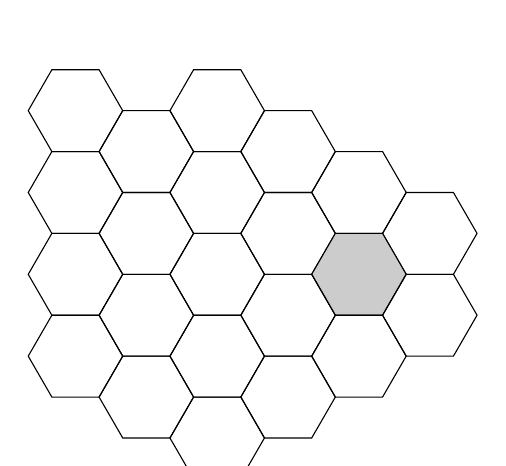
\begin{tikzpicture}
			      \begin{scope}[%
					      every node/.style={regular polygon,
							      regular polygon sides=6,
							      draw,
							      minimum width=1.2cm,
							      outer sep=0,
						      }, transform shape]
				      \node (A) {};
				      \node[anchor=west] (B) at (A.corner 5) {};
				      \node[anchor=west] (C) at (B.corner 1) {};
				      \node[anchor=west] (D) at (C.corner 5) {};
				      \node[anchor=west] (E) at (D.corner 5) {};
				      \node[anchor=west] (F) at (E.corner 5) {};
				      \node[anchor=west] (G) at (B.corner 5) {};
				      \node[anchor=west] (H) at (G.corner 5) {};
				      \node[fill=gray!40,anchor=west] (I) at (H.corner 5) {};% ini diarsir
				      \node[anchor=west] (J) at (I.corner 5) {};
				      \node[anchor=east] (K) at (B.corner 4) {};
				      \node[anchor=west] (L) at (K.corner 5) {};
				      \node[anchor=west] (M) at (L.corner 5) {};
				      \node[anchor=west] (N) at (M.corner 5) {};
				      \node[anchor=west] (O) at (N.corner 5) {};
				      \node[anchor=east] (P) at (L.corner 4) {};
				      \node[anchor=west] (Q) at (P.corner 5) {};
				      \node[anchor=west] (R) at (Q.corner 5) {};
				      \node[anchor=west] (S) at (R.corner 5) {};
				      \node[anchor=east] (T) at (Q.corner 4) {};
				      \node[anchor=west] (U) at (T.corner 5) {};
				      \node[anchor=west] (V) at (U.corner 5) {};
			      \end{scope}
		      \end{tikzpicture}
	      \end{center}
\end{enumerate}
\subsubsection*{URAIAN}
\begin{enumerate}
	\item  Misalkan $n$ adalah bilangan bulat 8 digit dengan digit pertama adalah 5. Berapakah peluang untuk mendapatkan $n$ yang memuat tidak lebih dari 5 digit berbeda?
	\item Diberikan barisan-barisan bilangan real $(x_n)$ dan $(y_n)$ dengan $(x_n)$ konvergen ke $x\in\R$, barisan $(y_n)$ konvergen ke $y\in\R$. Jika barisan $(z_n)$ didefinisikan dengan $z_n=\dfrac{1}{n}\displaystyle\sum_{i=1}^k x_iy_{n+1-i}$. Buktikan bahwa barisan $(z_n)$ konvergen ke $xy$.
	\item Diberikan fungsi kontinu $f:[0,1]\rightarrow\R$ memenuhi $\displaystyle(f(x))^2\leq 4\int_0^x (f(t))^2~dt$ untuk setiap $x\in[0,1]$. Buktikan bahwa $3(f(x))^2+2f(x)=0$ untuk setiap $x\in[0,1]$.
	\item \begin{enumerate}
		      \item  Berikan suatu contoh homomorfisma grup $\psi$ yang injektif dari grup $(\Z_6,+)$ ke grup $S_5$.
		      \item Ada berapa banyak homomorfisma grup dari grup $(\Z_6,+)$ ke $S_5$?
	      \end{enumerate}
	\item Diketahui $R$ merupakan suatu ring dengan identitas perkalian $1_R$ dan $(x+y)^2=x^2+y^2$ untuk setiap $x,y\in R$. Apakah $R$ merupakan ring komutatif?
\end{enumerate}
\newpage
\subsection{HARI KEDUA}
\begin{center}
	(ANALISIS KOMPLEKS, ALJABAR LINEAR, KOMBINATORIKA)
\end{center}
\subsubsection*{ISIAN SINGKAT}
\begin{enumerate}
	\item  Banyaknya bilangan asli kurang dari atau sama dengan 2023 yang memuat digit $0$ adalah \dots
	\item Misalkan $l$ garis di $\R^3$ yang merupakan perpotongan antara bidang $x+2y+3z=20$ dan bidang $x-y+z=23$. Jika garis $l$ memotong bidang$-xy$ di titik $P(a,b,c)$, maka nilai dari $a+b+c$ adalah \dots
	\item Misalkan I adalah operator identitas pada $\R^3$ dan $T:\R^3\rightarrow\R^3$ adalah operator linear yang memenuhi
	      \begin{align*}
		      T\begin{pmatrix}
			       \begin{bmatrix}
				      1 \\ 0 \\ 0
			      \end{bmatrix}
		       \end{pmatrix}=\begin{bmatrix}
			                     1 \\ 0 \\0
		                     \end{bmatrix}, \quad T\begin{pmatrix}
			                                           \begin{bmatrix}
				      1 \\ 1 \\ 0
			      \end{bmatrix}
		                                           \end{pmatrix}= \begin{bmatrix}
			                                                          1 \\ 2 \\ 0
		                                                          \end{bmatrix}
		      , \quad T\begin{pmatrix}
			               \begin{bmatrix}
				      1 \\ 1 \\ 1
			      \end{bmatrix}
		               \end{pmatrix}= \begin{bmatrix}
			                              1 \\ 2 \\ 3
		                              \end{bmatrix}
	      \end{align*}
	      Nilai dari $(T-I)\circ(T-2I)\circ(T-3I)\begin{pmatrix}
			      \begin{bmatrix}
				      9 \\ 7 \\ 8
			      \end{bmatrix}
		      \end{pmatrix}$  adalah \dots
	\item Banyak bilangan kompleks tak real $z$ yang memenuhi $|z-20|+|z-23|=3$ adalah \dots
	\item Nilai $m$ agar fungsi kompleks $f(z)=\dfrac{z-2023}{1-3z}$ memetakan lingkaran $|z-3|=m$ menjadi garis lurus adalah \dots
\end{enumerate}
\subsubsection*{URAIAN}
\begin{enumerate}
	\item  Tentukan semua bilangan real $a,b,c$ sehingga matriks
	      \begin{align*}
		      A=\begin{bmatrix}
			        1 & 2 & 3 \\
			        4 & 5 & 6 \\
			        a & b & c
		        \end{bmatrix}
	      \end{align*}
	      memiliki nilai eigen 2, 0, dan 23
	\item Misalkan $A$ matriks berukuran $n\times n$ dengan komponen real sedemikian sehingga vektor $Au$ dan $u$ ortogonal untuk setiap vektor $u\in\R^n$.
	      Buktikan bahwa $A^T=-A$.
	\item Misalkan $\omega\neq 1$ merupakan bilangan kompleks dengan sifat $w^7=1$. Tentukan semua bilangan bulat positif $n$ sehingga
	      \begin{align*}
		      \sum_{k=1}^n (1+\omega^k+\omega^{2k}+\omega^{3k}+\omega^{4k}+\omega^{5k}+\omega^{6k})=2023
	      \end{align*}
	\item Buktikan
	      \begin{align*}
		      |\tan(x+iy)| \geq \dfrac{|e^y-e^{-y}|}{e^y+e^{-y}} \qquad \text{untuk setiap } x,y\in \R
	      \end{align*}
	\item Dalam suatu turnamen terdapat 28 tim yang akan bertanding. Masing-masing tim bermain satu sama lain hanya sekali. Perolehan poin pada setiap pertandingan adalah 2 poin bagi pemenang, 0 poin bagi yang kalah, dan masing-masing 1 poin untuk kedua tim bila berakhir seri. Dalam turnamen tersebut, lebih dari 75\% pertandingan berakhir seri. Buktikan bahwa terdapat dua tim yang meraih total poin yang sama besar.
\end{enumerate}

\newpage
\lhead{ONMIPA-PT(2024)}
\section{ONMIPA-PT TINGKAT WILAYAH 2024}
\subsection{HARI PERTAMA}
\begin{center}
	(ANALISIS REAL, STRUKTUR ALJABAR, KOMBINATORIKA)
\end{center}
\subsubsection*{ISIAN SINGKAT}
\begin{enumerate}
	\item Jika $I$ koleksi interval buka pada $\R$ dengan $I=\{I_n:I_n=\qty(1,1+\frac{1}{n}),n\in\mathbb{N}\}$, maka $\displaystyle \bigcup_{I_n\in I} I_n=\cdots$ dan $\displaystyle \bigcap_{I_n\in I} I_n=\cdots$.
	\item Untuk setiap $n\in\mathbb{N}, f_n:[-1,1]\rightarrow \R$ dengan $f_n(x)=\cos(n\arccos x), x\in[-1,1]$. Untuk setiap dua bilangan asli $m$ dan $n$ dengan $m\neq n$, nilai $\displaystyle\int_{-1}^1 \dfrac{f_n(x)f_m(x)}{\sqrt{1-x^2}}\, dx=\cdots$
	\item Diberikan $G$ suatu grup siklis dengan orde 2024. Banyak elemen $G$ yang berorde ganjil adalah $\dots$.
	\item Jika $a,b,c,d$ merupakan bilangan bulat sehingga $f(x)=x^4+ax^3+bx^2+cx+d$ mempunyai akar $\sqrt{3}-\sqrt{5}$, maka nilai $a+b+c+d$ adalah \dots.
	\item Dalam sebuah kotak terdapat kelereng berwarna biru, hijau, merah, kuning, dan abu-abu dengan masing-masing warna terdapat 9 kelereng. Banyak cara mengambil 9 kelereng dari kotak sehingga setiap warna paling sedikit terambil satu kali adalah \dots.
\end{enumerate}
\subsubsection*{URAIAN}
\begin{enumerate}
	\item  Misalkan $a$ dan $b$ bilangan real positif yang memenuhi $\sqrt{b}<a<2\sqrt{b}$. Barisan bilangan real $(x_n)$ didefinisikan dengan $x_0\geq 0$ dan
	      \begin{align*}
		      x_n = \dfrac{ax_{n-1}+b}{x_{n-1}+a}, \quad \forall n\in\mathbb{N}
	      \end{align*}
	      Apakah $\displaystyle\lim_{n\rightarrow\infty} x_n$ ada? Jika ya, tentukan nilai limitnya.
	\item Diberikan fungsi kontinu $f:[a,b]\rightarrow \R$ dengan sifat untuk setiap $x\in[a,b]$ terdapat $p\in[a,b]$ dengan $|f(p)|\leq \dfrac{2023}{2024}|f(x)|$. Buktikan terdapat $c\in[a,b]$ dengan $f(c)=0$.
	\item Diketahui $R=\mathbb{Z}_{1013}\times \mathbb{Z}_{1013}$ merupakan ring terhadap operasi penjumlahan dan perkalian berikut:
	      \begin{align*}
		      (a,b)+(c,d)      & = ((a+c) \mod 1013, (b+d)\mod 1013)   \\
		      (a,c)\cdot (c,d) & = ( ac\mod 1013, (ad+bc+bd)\mod 1013)
	      \end{align*}
	      untuk setiap $(a,b),(c,d)\in R$. Buktikan terdapat tepat sebanyak 2024 elemen taknol di $R$ yang merupakan pembagi nol. (\textbf{Catatan:} 1013 bilangan prima).
	\item Suatu grup hingga $(G,\ast)$ berorde $n$ dikatakan \textit{rapi} jika terdapat $n$ unsur berbeda $g_1,g_2,\cdots, g_n$ sehingga $G=\{g_1\ast g_2, g_2\ast g_3,\cdots, g_{n-1}\ast g_n, g_n\ast g_1\}$
	      \begin{enumerate}
		      \item  Tunjukkan bahwa $(\mathbb{Z}_7, +)$ \textit{rapi}
		      \item Buktikan bahwa untuk setiap $n$ genap, $(\mathbb{Z}_n, +)$ \textbf{tidak} \textit{rapi}.
	      \end{enumerate}
	\item Tunjukkan bahwa jika $n+1$ bilangan bulat berbeda diambil dari himpunan $\{1,2,\cdots, kn\}$, maka selalu ada dua bilangan bulat yang selisihnya paling banyak $k-1$.
\end{enumerate}
\newpage
\subsection{HARI KEDUA}
\begin{center}
	(ANALISIS KOMPLEKS, ALJABAR LINEAR, KOMBINATORIKA)
\end{center}
\subsubsection*{ISIAN SINGKAT}
\begin{enumerate}
	\item Banyak bilangan kompleks \( z \) yang memenuhi \( z^{20} = 1 \) dan \( z^{24} \in \mathbb{R} \) adalah \dots

	\item Jika diberikan fungsi kompleks \( f(z) = \overline{z} e^{-|z|^2} \), maka nilai \( f'(i) \) adalah \dots

	\item Misal \( P_4 \) adalah ruang polinomial dengan koefisien real berderajat paling tinggi 4. Didefinisikan pemetaan \( T_k: P_4 \to P_4 \) dengan
	      \[
		      T_k \left( a_0 + a_1 x + a_2 x^2 + a_3 x^3 + a_4 x^4 \right) := a_0 + a_1^k x^2 + a_2 x^4.
	      \]
	      Banyak pasangan bilangan \( (k,m) \) dengan \( k,m \in \{1,2,3,4\} \) sehingga \( T_k^m \) pemetaan linear adalah \dots (Catatan: \( T_k^m := \underbrace{T_k \circ T_k \circ \dots \circ T_k}_\textit{sebanyak \( m \) kali} \).)

	\item Misalkan \( \mathbf{e_1}, \mathbf{e_2}, \dots, \mathbf{e_{10}} \) basis baku dari ruang vektor \( \mathbb{R}^{10} \). Tinjau dua himpunan
	      \(
	      U = \{ \mathbf{e_1}, \mathbf{e_2} + \mathbf{e_3}, \mathbf{e_4} + \mathbf{e_5} + \mathbf{e_6}, \mathbf{e_7} + \mathbf{e_8} + \mathbf{e_9} + \mathbf{e_{10}} \}
	      \)
	      dan
	      \(
	      V = \{ \mathbf{e_1} + \mathbf{e_2}, \mathbf{e_3} + \mathbf{e_4}, \mathbf{e_5} + \mathbf{e_6}, \mathbf{e_7} + \mathbf{e_8}, \mathbf{e_9} + \mathbf{e_{10}} \}.
	      \)
	      Dimensi terkecil dari subruang yang memuat \( U \) dan \( V \) adalah \dots

	\item Dalam kejuaraan catur yang diikuti oleh 10 peserta, setiap peserta bertanding dengan peserta lain tepat satu kali. Peserta yang menang, kalah, dan seri di setiap pertandingan, berturut-turut diberikan skor 2, 0, dan 1. Jika total skor setiap peserta di akhir kejuaraan berbeda-beda, maka maksimal banyak pertandingan yang mungkin dimenangkan oleh peserta dengan skor terendah adalah \dots.

\end{enumerate}

\subsubsection*{URAIAN}
\begin{enumerate}
	\item Untuk setiap bilangan kompleks \( z \) dengan \( |z| = 1 \), tunjukkan bahwa
	      \[
		      1 \leq |1+z| + |1+2z| \leq 5.
	      \]

	\item Tentukan daerah \( D \) di bidang kompleks sehingga untuk setiap \( z \in D \), \(\displaystyle\lim_{|z|\to\infty} e^z\) ada.

	\item Diberikan matriks
	      \[
		      A = \begin{bmatrix}
			      0 & a & 0 \\
			      a & b & a \\
			      0 & a & 0
		      \end{bmatrix}
	      \]
	      dengan \( a, b \in \mathbb{R} \) dan \( a \neq 0 \). Buktikan bahwa matriks \( A \) dapat didiagonalkan.

	\item Diberikan matriks
	      \[
		      A = \begin{bmatrix}
			      20 & 24 \\
			      p  & q
		      \end{bmatrix}
	      \]
	      dengan \( p \) dan \( q \) real. Selidiki apakah terdapat bilangan real \( p \) dan \( q \) agar ada \( \mathbf{b} \in \mathbb{R}^2 \) sehingga persamaan
	      \[
		      A^2 \mathbf{x} = A \mathbf{b}
	      \]
	      tidak memiliki solusi \( \mathbf{x} \in \mathbb{R}^2 \). Jika ada, sebutkan semua \( p \) dan \( q \) yang mungkin. Berikan penjelasan jawaban Saudara.

	\item Jika koefisien \( a \) dan \( b \) dari persamaan garis lurus \( ax + by = 0 \) adalah dua bilangan berbeda dari \( \{0,1,2,3,6,7\} \), tentukan banyaknya garis lurus berbeda yang dapat dibentuk.

\end{enumerate}


\end{document}
